\documentclass{article}
\usepackage[utf8]{inputenc}
\usepackage{multirow}
\usepackage{float}
\usepackage{graphicx}
\usepackage{siunitx}
\usepackage{tabto}
\usepackage{amssymb}
\usepackage[margin=2cm]{geometry}
\usepackage[english]{babel}
\usepackage{float}
\usepackage{graphicx}
%\usepackage{xcolor}
\usepackage{caption, subcaption}
\usepackage{fancyhdr}
\usepackage{array}
\usepackage{adjustbox}
\usepackage{caption}
\usepackage[table]{xcolor}
\usepackage[hidelinks=true]{hyperref}
\usepackage{gensymb}
\usepackage{lastpage}
\newcommand{\HRule}[1]{\rule{\linewidth}{#1}}
\usepackage{xurl}
\usepackage[export]{adjustbox}
\usepackage{wrapfig}
\usepackage{amsmath}
\usepackage{multirow}
\usepackage{pdfpages}
\usepackage{xcolor}
\usepackage{booktabs}
\usepackage{color}

\geometry{
 a4paper,
 total={170mm,247mm},
 left=20mm,
 top=20mm,
 }
\usepackage{pdflscape}
\usepackage{pdfpages}

\begin{document}

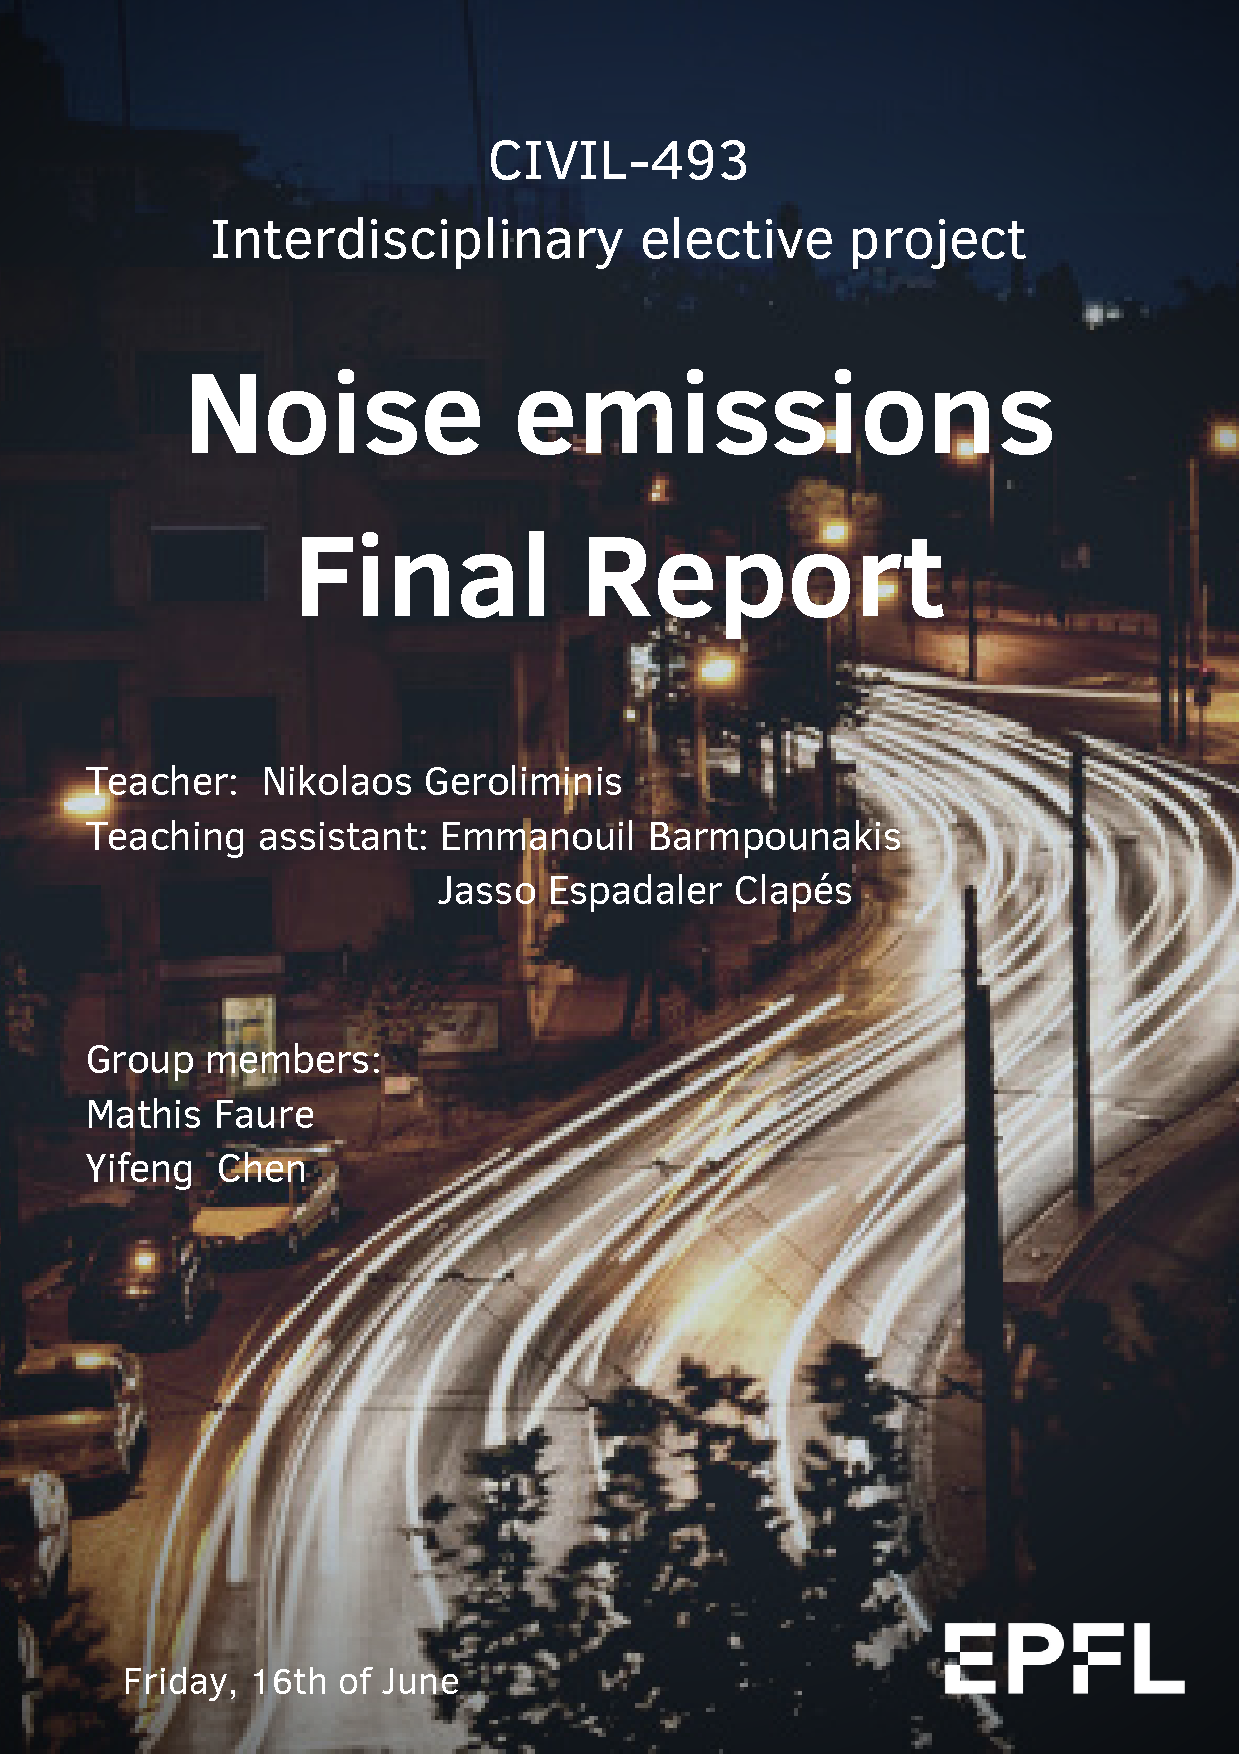
\includepdf[pages={1}]{noise_emissions_cover_page.pdf}

%\maketitle

% \begin{figure}[h]
%    \centering
%    \includegraphics[scale=0.5]{logo_EPFL.png}
% \end{figure}


\pagebreak
\tableofcontents
\pagebreak
\pagenumbering{arabic}


\section{Introduction}

\noindent In the European Union, 72,5\% of the population, or almost 340 million people, live in urban areas \cite{Pop_in_cities}. 446 cities each have more than 100,000 inhabitants \cite{Cities_with_more_than_100_habs}. This concentration raises major questions about the organization of urban space in order to offer an acceptable quality of life to city dwellers. Indeed, with such high densities (around 3,000 inhabitants$/km2$ and {\color{red} 17500 inhabitants$/km2$} for the city of Athens for example \cite{European_city_density}), several forms of pollution degrade the urban environment. Of the sources of discomfort perceived by city dwellers, noise is the phenomenon that causes the most discomfort after air pollution \cite{Noise_emissions_effects}. This noise is the result of human activities, mainly coming from transport, whether road, rail or air. \\
The impact of noise exposure on the body has been observed and studied for many years. Sleep disturbance, loss of alertness and concentration, increased stress, blood pressure and heart rate are the most commonly observed side effects \cite{Noise_emissions_effects}. This health impact comes at a financial cost to society. In addition, if noise in the city impacts the lives of city dwellers, it also affects wildlife, causing them stress or complicating communication between individuals and their reproduction. {\color{red} To overcome these problems some laws have been put in place at the European level such as the directive 2002/49/EC which regulates the emissions emitted by vehicles according to their location (see figure \ref{European noise emissions directive}).}\\
It is therefore necessary and useful to know how to characterize the urban sound environments (USE) in order to estimate the sound sources present, their sound levels and their distribution in order to reduce and limit their impacts on the urban populations. \\

\noindent By placing microphones close to main roads recording the different noises emitted by vehicles as well as the characteristics specific to different types of vehicles (heavy goods vehicles, medium-heavy goods vehicles, etc.), teams of engineers have developed models allowing to approximate the noise emissions of vehicle fleets based on data from the field. \\
\noindent {\color{red}The use of drones, which has developed considerably in recent years, has made it possible to collect the data required as input for the various noise emission prediction models. 
It is now possible with a fleet of drones to collect a sufficient amount of information to determine the noise emissions of a fleet of vehicles, over a defined area, for a period of time up to several hours.
A major advantage of this approach is the reduction in the amount of labor required. A small number of people are now needed to operate the drones and plan the experiment, as opposed to the large number of people initially needed to hold the many microphones needed to collect the data (see figure \ref{City noise emissions monitoring}). Moreover, the data collected with the help of drones can now also be used to calculate the greenhouse gas emissions as well as the different road flows present on the network.
} \\

\noindent Initially, three sound emission models (NMPB, IMAGINE and CNOSSOS) will be studied (see figure \ref{Noise emissions models}. \cite{Can2018} Their differences and common points as well as their advantages and disadvantages will be detailed.
In a second step, the results obtained for the different models will be analyzed. To conclude, suggestions will be made to improve the various models already in place. \\

{\color{red}
\section{Noise emissions definition}
\noindent First of all noise emissions are loud or unpleasant sound that are released into the atmosphere \cite{Noise_emissions_definition}. \\
The intensity of a sound is measured in decibel. The decibel scale measures noise logarithmically, which is similar to how our ears perceive sound. \\
The abbreviation for decibel is dB. A value expressed in dB(A) is the evaluation in decibels of a sound level with the A-weighting of the standard IEC 61672-1 "Electroacoustics - Sound Level Meters ", established to take into account the average sensitivity, at a low sound volume, of people with a hearing considered normal, for each frequency band.\\
To measure sound intensity we can use a sound level meter (SLM).\\
To have an idea of the different orders of magnitude, we can assimilate certain values to certain sounds of everyday life. For example, people speak at an intensity of 30dB, a car driving produces 70dB against 120dB for a police car \cite{Mesure_noise_emissions}. 

\begin{figure}[H]
    \begin{center}
        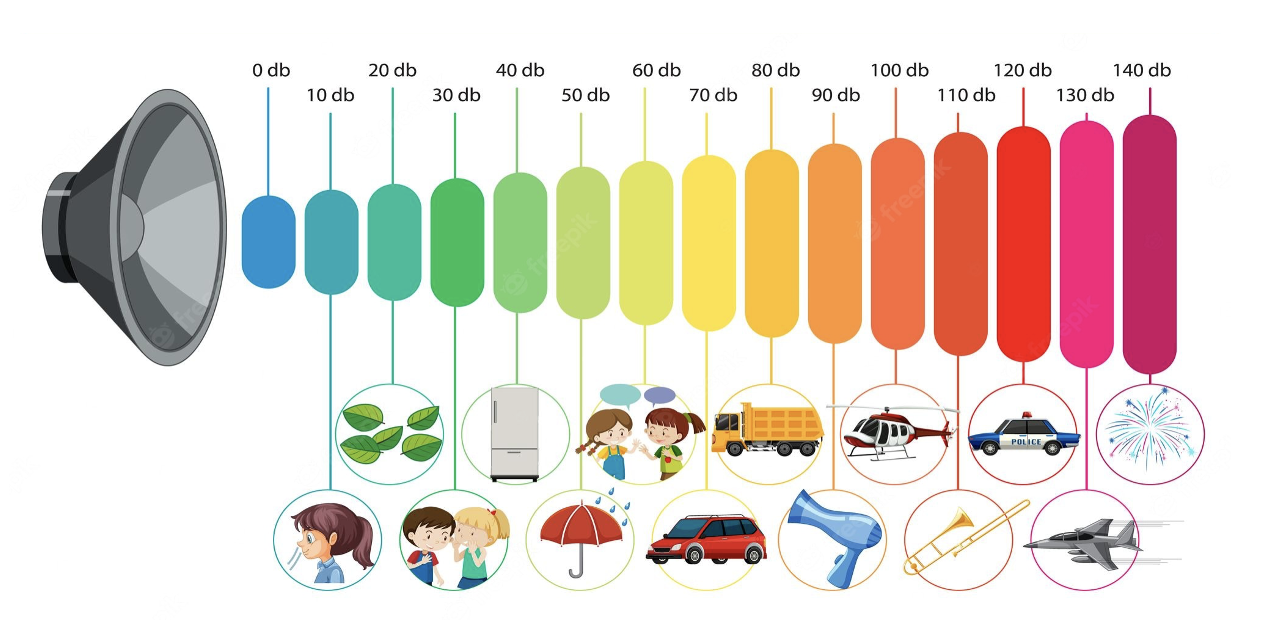
\includegraphics[width=14cm]{Decibel scale.png}
        \caption{Decibel scale}
        \label{Decibel scale}
    \end{center}
\end{figure} }

\section{Data preprocessing}

\subsection{pNEUMA dataset}

\noindent pNEUMA is a large-scale open dataset featuring the trajectories of half a million vehicles that were collected in an experiment by a {\color{red} swarm} of drones in the congested downtown area of Athens, Greece \cite{Pneuma_data_set}. This unique observatory, at a scale an order of magnitude larger than previously available, allows for the development of new models based on trajectories, vehicle type, and roadway geometry. \\
\noindent In this study, the various data collected by drone number 8 over a period of 15 minutes during a peak traffic period will be used to predict vehicle noise emissions by applying the models detailed above.

\subsection{Removing outliers}

The first step is to eliminate outliers. As the data is collected in an urban environment (the city center of Athens), speed values above 130 km/h do not seem realistic. Only three vehicles have these characteristics {\color{red} and therefore are excluded from the analysis.}

\subsection{Granularity}

The data collected by the drone flying over the area have a granularity of 0.04s or 40ms. In the context of our studies such a fine granularity is not necessary and greatly increases the computation time performed by the computer. In order to optimize the results obtained a granularity of 1s was chosen for the rest of the experiment.

\section{Noise emissions models}

\subsection{NMPB model ('Nouvelle Méthode de Prévision du Bruit'}

\noindent NMPB-Routes-2008 is the French road noise prediction method derived from the experimental method NMPB-Routes-1996 \cite{Hamet2010}. It is used for the application of national legislation on noise from land transport infrastructures, for various impact studies and was used until December 31, 2018 for the application of the 2002 "noise" directive. Since this date, the model specified in the directive 2015/996/EC, known as the "CNOSSOS-EU" model, must be used for the creation of strategic noise maps (SNM).

\subsubsection{Road noise and source origin}

\noindent The part of the NMPB concerning emission proposes a method of predictive calculation of road noise distinguishing three categories of pavement performance. The categories were defined on the basis of a statistical analysis of the national database of acoustic performances of pavements, managed by the Strasbourg laboratory (Cerema Est).\\
Three classes have been defined in relation to rolling noise levels measured by the method at 90 km/h: 
\begin{itemize}
    \item Class R1 for "low noise" pavements with an average of less than 76 dB(A) ;
    \item Class R2 for "intermediate" pavements with an average above 76 dB(A) Class R2 for "intermediate" pavements with an average of more than but less than 79 dB(A) ;
    \item Class R3 for "noisy" pavements with an average of more than 79 dB(A).
\end{itemize}

\begin{figure}[H]
\caption{Segmentation of pavements into 3 categories of acoustic performance
}
\label{Segmentation of pavements}
\centering
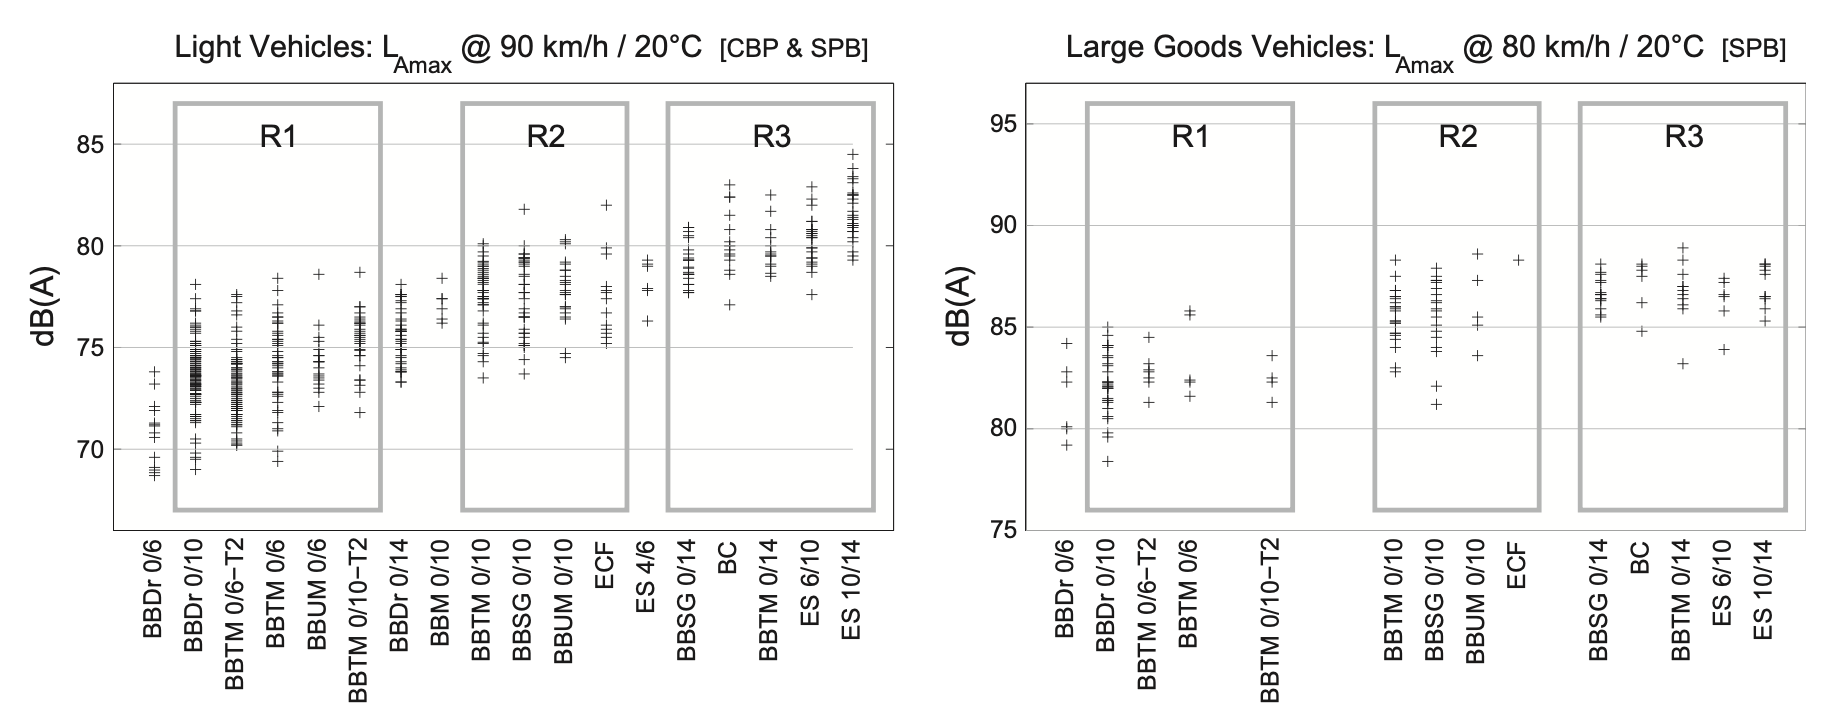
\includegraphics[width=1\textwidth]{NMPB/Pavement_segmentation.png}
\end{figure}

{\color{red} \noindent As the acoustic performance categories were not known on the studied road network, an intermediate category was chosen (R2) based on the quality of the asphalt observed with the help of tools such as Google maps or the maintenance of the roads in a developed country but having undergone repeated economic crises in recent years.\\}

\noindent Road noise is the sound energy emitted by all vehicles in the traffic. It depends on the number of vehicles in the traffic and their noise emission characteristics. \\ 
\noindent Vehicles are grouped into categories with similar noise characteristics. {\color{red} In order to apply the NMPB model it is necessary to classify the different types of vehicles observed in the field (Taxi, Medium Vehicle, Motorcycle, Car, Bus and Heavy Vehicle) into two categories. The GdBN08 splits the vehicles into two categories : light vehicles (LV, below 3.5 t) and heavy vehicles (HV, 3.5 t and above). Taxis, medium vehicles, motorcycles, and cars will be considered as light vehicles. Buses and trucks will be considered as heavy vehicles.}\\

\noindent For a vehicle, noise sources come from:
\begin{itemize}
    \item From the mechanical system: propulsion noise component (PNC) from the engine, transmissions and exhaust;
    \item From the tire-road contact: rolling noise component (RNC). 
\end{itemize}

\noindent Aerodynamic noise, which is supposed to be significant at speeds above 130 km /h, is generally neglected or integrated in the rolling noise. \\

\noindent For motorized two-wheelers, rolling noise is negligible. The noise emission comes mainly from the engine and the exhaust system (if thermal engine).

\subsubsection{General principles of the road noise emission model}

\noindent The emission model predicts sound levels in one-third octave bands from 100 Hz to 5000 Hz and allows for the following parameters: 
\begin{itemize}
    \item Vehicles:
    \begin{itemize}
        \item Vehicle category: light vehicles (LV) and heavy vehicles (HV);
        \item Acceleration: stabilized, accelerated, decelerated ;
        \item Speed: from 20 km /h (5 km /h in acceleration/deceleration) to 130 km /h (resp. 110 km /h) for LV (resp. HV)
    \end{itemize}
    \item Roadway :
    \begin{itemize}
        \item Slope: slope [from -6\% to -2\%], flat [from -2\% to 2\%], ramp [from 2\% to 6\%] ;
        \item Pavement category: R1, R2, R3 ;
        \item Coating age: less than 2 years, aging law of 2 to 10 years.
    \end{itemize}
\end{itemize}

\subsubsection{Source equations}

\noindent For rolling noise, the emission $L_{r,R}$ is formulated as follows:

\begin{equation}
    \label{RNC_LV}
    \centering
    \begin{aligned}
        L_{r,R}(v) = A_R+B_R\log(\frac{v}{v_{ref}}) \\
        \text{ where } v_{ref}=90km/h \text{ for LVs and } v_{ref}=80km/h \text{ for HVs}
    \end{aligned}
\end{equation}


\noindent The two main components can be {\color{red} obtained} from the following table:

\begin{table}[H]
\centering
\caption{Rolling noise components of the three road surface}
\label{Rolling noise components of the three road surface}
\begin{tabular}{c|cccc|}
\cline{2-5}
                         & \multicolumn{2}{c}{LV} & \multicolumn{2}{c|}{HV} \\
                         & A_R       & B_R      & A_R       & B_R       \\ \hline
\multicolumn{1}{|c|}{R1} & 73,3       & 31,0      & 82,5       & 30         \\
\multicolumn{1}{|c|}{R2} & 77,3       & 30,1      & 85,6       & 30         \\
\multicolumn{1}{|c|}{R3} & 79,8       & 31,4      & 86,6       & 30         \\ \hline
\end{tabular}
\end{table}


\noindent For propulsion noise, the emission $L_{p}$ is formulated as follows:

\begin{equation}
    \label{RNC_LV}
    \centering
    \begin{aligned}
        L_{p}(v) = L_{p}(v_{ref})+b\log(\frac{v}{v_{ref}}) \\
        \text{ where } v_{ref}=90km/h \text{ for LVs and } v_{ref}=80km/h \text{ for HVs}
    \end{aligned}
\end{equation}

\noindent The two main components can be {\color{red} obtained} from the following tables depending {\color{red} on} the type of the vehicle and its acceleration state:

\begin{table}[H]
\centering
\caption{PU noise component, LV, steady condition}
\label{PU noise component, LV, steady condition}
\begin{tabular}{|lllll|}
\hline
v & km/h  & 20-30 & 30-110 & 110-130 \\ \hline
$L_{p,LV}(90)$ & dB(A) & 60,6  & 66,3   & 64,6    \\
b & dB(A)/decade & 0     & 12,0   & 31,3    \\ \hline
\end{tabular}
\end{table}

\begin{table}[H]
\centering
\caption{PU noise component, LV, acceleration}
\label{PU noise component, LV, acceleration}
\begin{tabular}{|lllll|}
\hline
v & km/h  & 5-20 & 20-100 & 100-130 \\ \hline
$L_{p,LV}(90)$ & dB(A) & 85,7 & 70     & 68,2    \\
b & dB(A)/decade & 24,1 & 0      & 38,6    \\ \hline
\end{tabular}
\end{table}

\begin{table}[H]
\centering
\caption{PU noise component, LV, deceleration}
\label{PU noise component, LV, deceleration}
\begin{tabular}{|lllll|}
\hline
v & km/h  & 5-20 & 20-100 & 100-130 \\ \hline
$L_{p,LV}(90)$ & dB(A) & 85,7 & 70     & 68,2    \\
b & dB(A)/decade & 24,1 & 0      & 38,6    \\ \hline
\end{tabular}
\end{table}

\noindent In the case of heavy vehicles, the acceleration of the vehicle is not taken into account but a factor related to the slope of the road must be taken into account. 

\begin{table}[H]
\centering
\caption{PU noise component, HV, steady speed}
\label{PU noise component, HV, steady speed}
\begin{tabular}{|llll|}
\hline
v & km/h         & 5-70 & 70-100 \\ \hline
$L_{p,HV}(80)$ & dB(A)        & 73   & 73     \\
b & dB(A)/decade & 0    & 13,0   \\ \hline
\end{tabular}
\end{table}

\begin{table}[H]
\centering
\caption{PU noise component. HV category correction term in dB(A)}
\label{PU noise component. HV category correction term in dB(A)}
\begin{tabular}{|llll|}
\hline
s(\%)        & \begin{tabular}[c]{@{}l@{}}Horizontal \\ 0-2\end{tabular} & \begin{tabular}[c]{@{}l@{}}Uphill `\\ 2-6\end{tabular} & \begin{tabular}[c]{@{}l@{}}Downhill\\ 2-6\end{tabular} \\ \hline
Steady speed & 0 & $2*(s-2)$  & $s-2$  \\
Acceleration & 5 & $5 + max[2*(s-4.5), 0]$ & 5 \\
Deceleration & 0 & 0 & $s-2$                                                    \\ \hline
\end{tabular}
\end{table}

{\color{red} \noindent To be able to use the table \ref{PU noise component. HV category correction term in dB(A)}, it is necessary to know the acceleration state of the vehicle for each time interval.
The status depends directly on the value of the acceleration captured by the drone. The relation between this observed value and the corresponding state will be defined according to the following table:

\begin{table}[H]
\centering
\caption{Acceleration states}
\label{Acceleration states}
\begin{tabular}{|c|c|c|}
\hline
Decelerating                     & Accelerating                        & Steady condition           \\ \hline
a \textless -0,5                 & a \textgreater 0,5                  & \multirow{2}{*}{Otherwise} \\
a \textless 0 and v \textless 20 & a \textgreater 0 and v \textless 20 &                            \\ \hline
\end{tabular}
\end{table}

\noindent Knowing that the category of acoustic performance of our road is R2 it is possible to determine the rolling noise parameter for each time-step and each vehicle with the help of tables \ref{Rolling noise components of the three road surface} and equation \ref{RNC_LV}.

\begin{equation}
    \label{RNC_LV2}
    \begin{aligned}
        L_{r,R,LV}(v) = 77,3+30,1\log(\frac{v}{90})
    \end{aligned}
\end{equation}


\begin{equation}
    \label{RNC_HV2}
    \begin{aligned}
        L_{r,R,HV}(v) = 85,6+30\log(\frac{v}{80})
    \end{aligned}
\end{equation}

\noindent The second term: the propulsion noise parameter must be calculated. However, for speeds lower than 5 km/h, in the case where the vehicle is in acceleration or deceleration phase, or if the vehicle has a speed lower than 20 km/h and has a constant acceleration, the standard does not define the values taken by the different parameters. These parameters will be equalized to 0, even if this will tend to underestimate the noise emitted by the vehicles.

If $v<5$ km/h and $(a<-0,5 or a>0,5)$ or if $v<20$ and $-0,5<a<0,5$:
\begin{equation}
    \label{RNC_v<5}
    \begin{aligned}
        L_{r,R,HV}(v) = 0 
    \end{aligned}
\end{equation}

\begin{equation}
    \label{PNC_LV2}
    \begin{aligned}
        L_{p,LV}(v) = L_{p,LV}(90)+b*\log(\frac{v}{90})
    \end{aligned}
\end{equation}

\begin{equation}
    \label{PNC_HV2}
    \begin{aligned}
        L_{p,HV}(v) = L_{p,HV}(80)+b*\log(\frac{v}{80})
    \end{aligned}
\end{equation}
}

\noindent Noise emission modeling is based on the aggregation of "road noise" and "engine noise" components for each vehicle category. The formulations of these components are derived from vehicle emission measurements that have been updated from previous reference methods (notably the 1980 "Guide du Bruit des Transports Terrestres" and the NMPB 96) to take into account changes in the vehicle flee and road surfaces. It is interesting to use this method in order to estimate the orders of magnitude of the acoustic performance of pavements according to the influencing parameters (type of vehicle, speed, inclination, etc.) \\
Measurement results are pass-by maximum levels in dB(A), $L_{Amax}$, measured at 7.5 m horizontal distance from the traffic path and 1.2 m height above the ground surface.

\begin{equation}
    \label{LAmax}
    \begin{aligned}
        L_{Amax} = L_{p} \oplus L_{r} = 10\log(10^{0,1*L_p}+10^{0,1*L_r})
    \end{aligned}
\end{equation}

\subsection{IMAGINE model}

\noindent {\color{red} The IMAGINE model was developed at the same time as the NMPB model but on a European scale.} Deliverable 11 of the European IMAGINE project formulates a model for the 25 to 10,000 Hz octave thirds.\cite{Box2004} \\

\subsubsection{General principles of the road noise emission model}

In this model, the sound power level of a vehicle is independent of the age of the pavement and the spectral distribution is speed dependent. \\
The structure of the model is defined on the basis of reference conditions: 
\begin{itemize}
    \item Constant velocity ;
    \item Horizontal route ;
    \item Temperature of 20°C ;
    \item Dry pavement;
\end{itemize}
    
\noindent From this reference configuration and according to the needs, corrections are applied on the rolling term of the model among which: 

\begin{itemize}
    \item The influence of the temperature ;
    \item The nature of the road surface.
\end{itemize}

\noindent The motor term of the model is also corrected for: 
\begin{itemize}
    \item The effect of acceleration ;
    \item The gradient;
    \item The nature of the pavement to take into account the possible sound absorption phenomena by the pavement.
\end{itemize}

{\color{red}\subsubsection{The octave and the 1/3 octave band frequencies}

\noindent The audible frequency range can be separated into unequal segments called octaves. \\

\noindent An octave higher is a doubling of the octave band frequency. Octave bands can be separated into three ranges - referred to as one-third-octave bands.

\begin{figure}[H]
    \begin{center}
        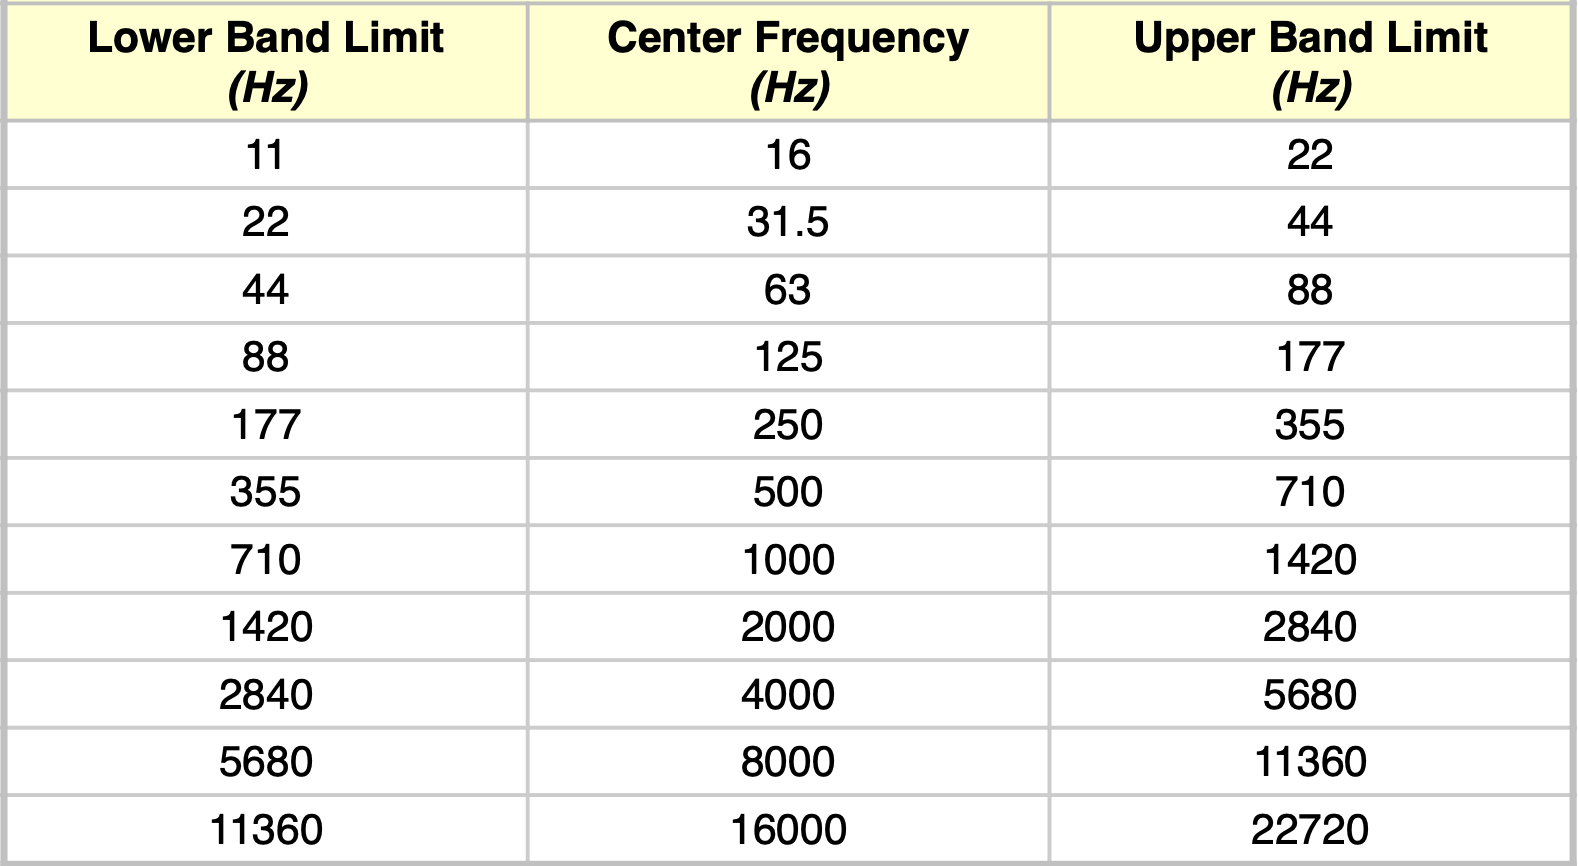
\includegraphics[width=0.8\textwidth]{IMAGINE/octave_band.png}
        \caption{Octave bands frequencies}
        \label{Octave bands frequencies}
    \end{center}
\end{figure}

\noindent The data was collected by a drone that does not have the ability to monitor octave band frequencies, so it is impossible to use the tables in the figure. \\
To overcome this problem two parallel studies are conducted. The first using the minima observed on the figures and the second the maxima. This allows to establish a confidence interval which will be analyzed later. }

\subsubsection{Source equations}

Like the French model, this model distinguishes between a rolling component and a propulsion component, with the difference that these components are dependent on the octave third considered (\ref{A and B coefficient}). \\

\noindent For rolling noise, the emission $L_{WR}$ is formulated as follows:



\begin{equation}
    \label{RNC_IMAGINE}
    \begin{aligned}
        L_{WR}(v) = A_R+B_R\log(\frac{v}{v_{ref}}) \\
        \text{ where: } v_{ref}=70 \text{km/h}
    \end{aligned}
\end{equation}

\noindent The aerodynamic noise of the vehicle is incorporated in this rolling noise equation.\\
\\

\noindent The propulsion noise emission $L_{WP}$ is formulated as follows:
\begin{equation}
    \label{RNC_IMAGINE}
    \begin{aligned}
        L_{WP}(v) = A_P+B_P\log(\frac{v-v_{ref}}{v_{ref}})+ \Delta L_{WP,acc} 
        
    \end{aligned}
\end{equation}
%\text{ where: } v_{ref}=70 \text{km/h}
        %\text{ and } \Delta L_{WP,acc} \text{ is the acceleration / deceleration correction factor}
\noindent These formulas, together predict the sound power level emitted by a road vehicle as a function of speed, under the reference condition, measured at 7.5 m horizontal distance from the traffic path and 1.2 m height above the ground surface (see equation \ref{LAmax}).\\

\noindent For four categories of vehicles: light vehicles (Category 1), medium heavy vehicles (Category 2), heavy vehicles (Category 3), motorized two-wheelers (Category 4), the norm contains graphs representing the spectra of the four main coefficients which give the intercept and the slope of each law.

\newpage

\begin{figure}[H]
\caption{A and B coefficient for rolling and propulsion noise, for all categories}
\label{A and B coefficient}
\centering
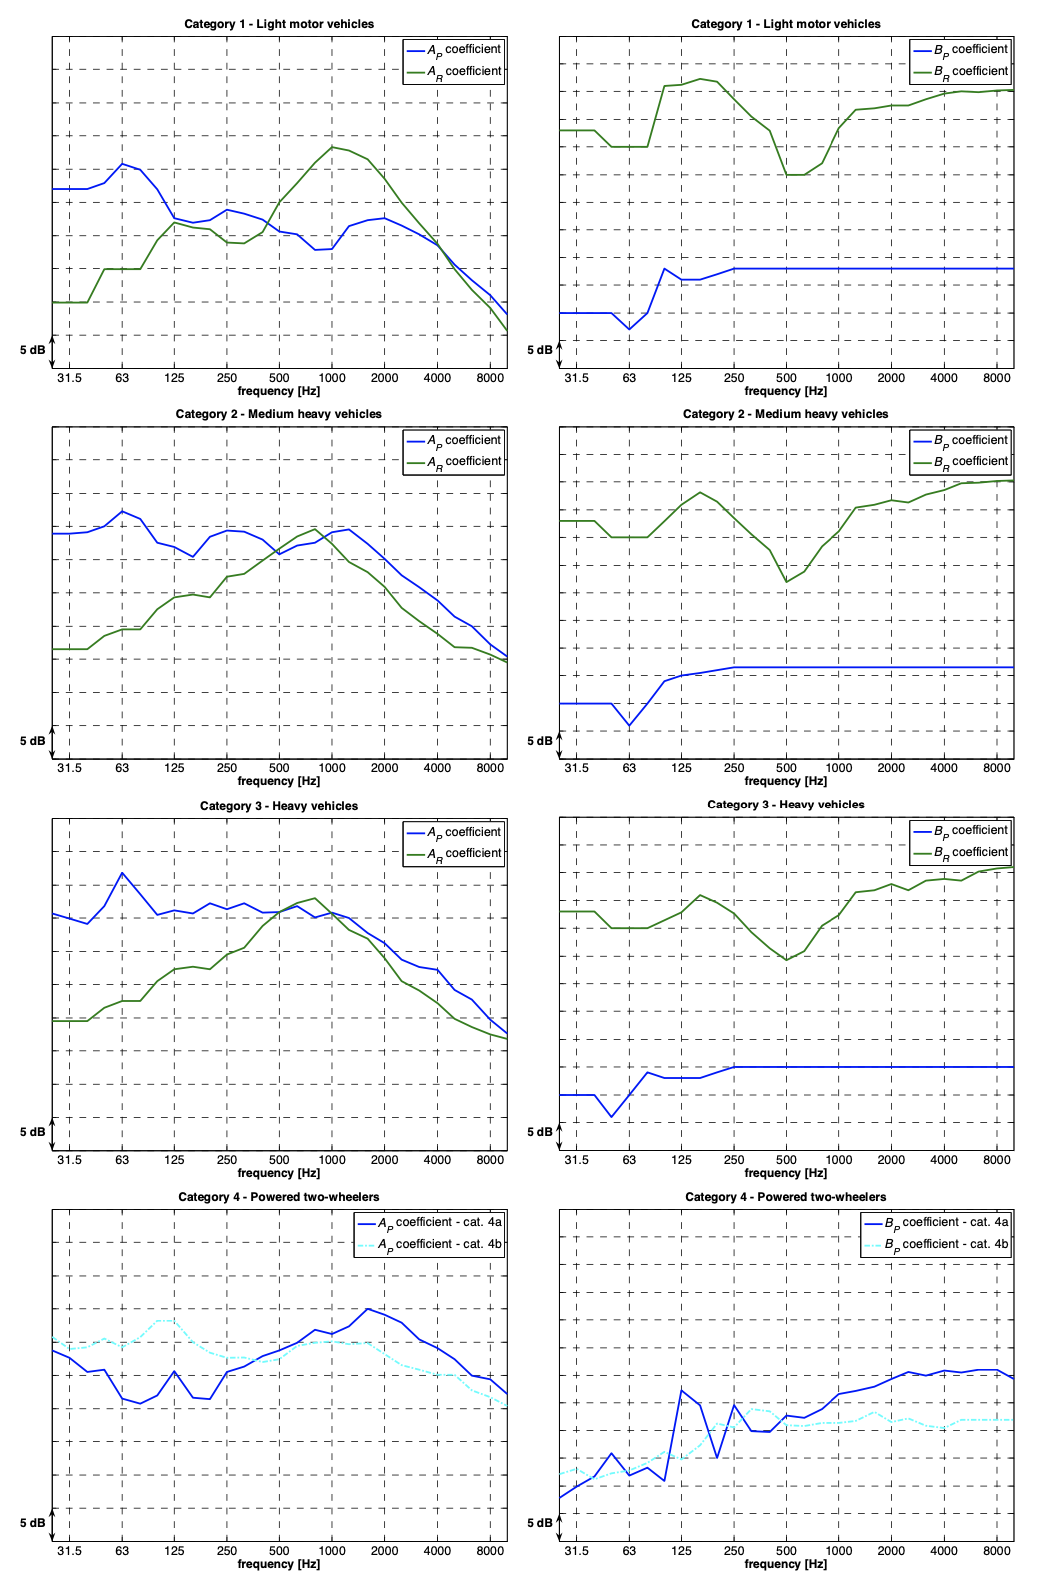
\includegraphics[scale=0.92]{IMAGINE/A and B coefficient for rolling and propulsion noise, for all categories.png}
\end{figure}

\subsubsection{Define an origin for the ordinate axis of the tables}

\noindent {\color{red} Graphs \ref{A and B coefficient} do not have a Y-axis origin.} The only information available is that the difference between 2 consecutive graduations is 5 dB. For the light and heavy vehicle categories, the spectra indicate that engine noise dominates at low frequency. One can question the abrupt fluctuations that appear on these spectra. It is true that the extent of the experimental base for this model is not known. \\
{\color{red} In order to obtain a reference, a parallelism has been made with the CNOSSOS method. The two methods being perfectly similar except for the correction factor related to the acceleration, based on the tables giving the values of the parameters for the equations of the PNC and the RNC, it is possible to determine the origin of the various figures of the IMAGINE norm.}

\subsubsection{Propulsion noise correction – Vehicle acceleration / deceleration}

\noindent For the propulsion noise accelerating and decelerating vehicles, a correction $L_{WP,acc}$ is developed based on instantaneous vehicle acceleration in $m/s^2$:


\begin{equation}
    \label{LAmax}
    \begin{aligned}
        \Delta L_{WP,acc} =
        \begin{cases}
        C_p*a       & \quad \text{for } a>=-1 m/s^2 \\
        C_p*(-1)  & \quad \text{for } a<-1 m/s^2
        \end{cases} \text{ with } |a|<=a_{max}
    \end{aligned}
\end{equation}

\noindent This correction is only valid for moderate acceleration values, as is expressed by the last expression. Here, $a_{max}$ is equal to 2 $m/s^2$ for category 1, 1 $m/s^2$ for categories 2 and 3, and 4 $m/s^2$ for category 4. \\
The coefficient $C_P$ is given for each 1/3-octave frequency band and for each vehicle category. The coefficient is equal for categories 1 and 4, as well as for categories 2 and 3.

\begin{figure}[H]
\caption{Acceleration coefficient $C_P$}
\label{Acceleration coefficient C_P}
\centering
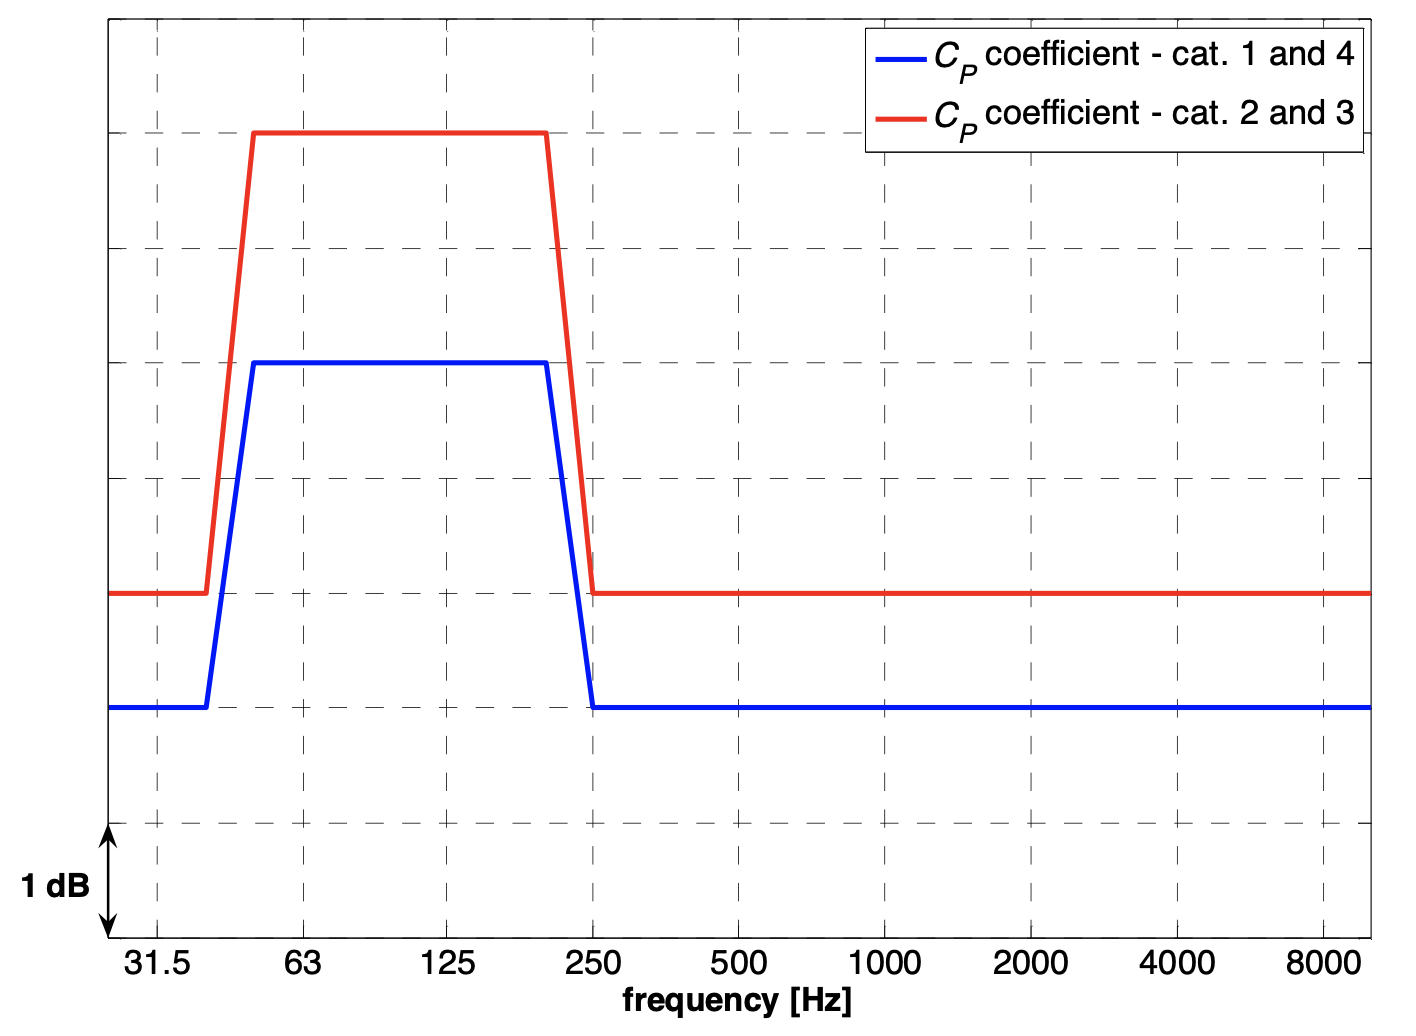
\includegraphics[width=0.8\textwidth]{IMAGINE/Acceleration coefficient C_P.png}
\end{figure}

\noindent Once again, unfortunately, the graphs in question is not scaled absolutely on the ordinate. The only information available is that the difference between 2 consecutive graduations is 1 dB.

\subsubsection{Acceleration correction factor : outside values}

\noindent The acceleration correction factor correction is only valid for moderate acceleration values. $a_{max}$ is equal to $2 m/s2$ for category 1, 1 $m/s2$ for categories 2 and 3, and 4 $m/s2$ for category 4. However, by observing the data, some values exceed the maximums defined by the norm.\\
In order to consider those vehicles whose acceleration or deceleration reach high values, their parameter $a$ will be equalized to $a_{max}$ according to the category to which they belong.\\

\noindent As explained before, this factor is not optimal for the studied road network. The implementation of a more recent method taking into account any type of acceleration or deceleration is necessary.




\subsection{CNOSSOS}
{\color{red}
\noindent The European CNOSSOS-EU method also defines the same four categories of vehicles \cite{Kephalopoulos2012}.} \\

\noindent As for the other models, the noise emissions of a road vehicle comes from two main sources: 

\begin{itemize}
    \item Tire/road contact noise;
    \item Propulsion noise produced by the vehicle's drive train (engine, transmission, etc.).
\end{itemize}

\noindent For motorized two-wheelers, tire/road contact noise is considered as for the other models as negligible. In this European model, the sound power level of a vehicle is independent of the age of the pavement and the spectral distribution is speed dependent. \\
The model is defined in octave bands from 63 to 8000 Hz. \\
The structure of the model is defined on the same basis of reference conditions as for the IMAGINE model. \\
\noindent From this reference configuration and according to the needs, corrections are applied on the rolling and propulsion term as for the IMAGINE model.
However in this case the acceleration as also an effect on the rolling term.

\subsubsection{Propulsion noise correction – Vehicle acceleration / deceleration}

\noindent Acceleration and deceleration of vehicles may have a significant effect on vehicle noise emission, especially when approaching or departing from road crossings. However, at the scale of a traffic flow, this effect is much more difficult to estimate than for individual vehicles, as it depends on the behaviour of individual vehicles, location, time, traffic conditions, etc... \\
\noindent For the rolling noise and the propulsion noise of accelerating and decelerating vehicles on a flat road, corrections $\Delta L_{WR,acc,i,m}$ and $\Delta L_{WP,acc,i,m}$ are developed from calculations based on the distance x (in m) from the point source to the nearest intersection of the respective source line with another source line. The correction term is attributed to all octave bands equally:

\begin{equation}
    \label{Delta L_R}
    \begin{aligned}
        \Delta L_{WR,acc,i,m} = C_{R,m,k}* \max(1-\frac{|x|}{100} ;0)
    \end{aligned}
\end{equation}

\begin{equation}
    \label{Delta L_P}
    \begin{aligned}
        \Delta L_{WP,acc,i,m} = C_{P,m,k}* \max(1-\frac{|x|}{100} ;0)
    \end{aligned}
\end{equation}

\noindent The coefficients $C_{R,m,k}$ and $C_{P,m,k}$ depend on the kind of junction k ($k = 1$ for a crossing with traffic lights ; $k = 2$ for a roundabout) and are given in the following tables for each vehicle category.

\begin{figure}[H]
\caption{Coefficients for acceleration and deceleration effect}
\label{Coefficients for acceleration and deceleration effect}
\centering
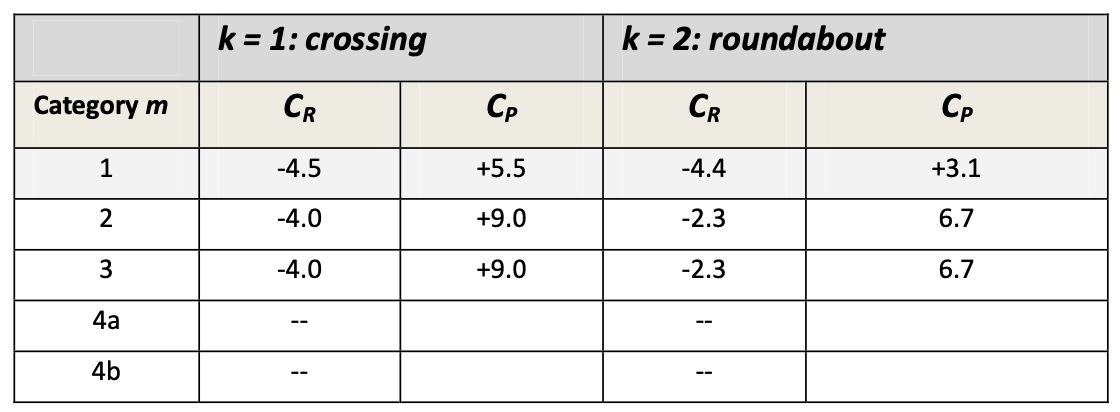
\includegraphics[width=0.65\textwidth]{CNOSSOS/Coefficients for acceleration and deceleration effect.png}
\end{figure}

{\color{red}
In the studied area there is no roundabout, only intersections. The k-factor will therefore be equalized to 1 which corresponds to intersections with traffic lights. \\
This distance is kept below 100 meters for all vehicles due to the geometry of the road network and the acceleration correction factor will never be zero. \\
The closer a vehicle is to an intersection the greater the factor will be. This means that moving away from or towards an intersection has the same impact on noise emissions. The effect of acceleration or deceleration on vehicle noise is therefore the same. \\
However, this model is simplistic because it does not take into account vehicle acceleration. A vehicle driving at constant speed and having a constant acceleration and taking advantage of the green-wave on an avenue will see its noise emissions changing while it is not the case in reality.}

\subsubsection{Source equations}

\noindent For rolling noise, the emission $L_{WR}$ is formulated as follows:

\begin{equation}
    \label{RNC_IMAGINE}
    \begin{aligned}
        L_{WR}(v) = A_R+B_R\log(\frac{v}{v_{ref}}) \\
        \text{ where: } v_{ref}=70 \text{km/h}
    \end{aligned}
\end{equation}

\noindent The aerodynamic noise of the vehicle is incorporated in this rolling noise equation.\\
\\

\noindent The propulsion noise emission $L_{WP}$ is formulated as follows:


\begin{equation}
    \label{RNC_IMAGINE}
    \begin{aligned}
        L_{WP}(v) = A_P+B_P\log(\frac{v-v_{ref}}{v_{ref}})+ \Delta L_{WP,acc} \\
        \text{ where: } v_{ref}=70 \text{km/h}
    \end{aligned}
\end{equation}

\noindent These formulas, together predict the sound power level emitted by a road vehicle as a function of speed, under the reference condition, measured at 7.5 m horizontal distance from the traffic path and 1.2 m height above the ground surface (see equation \ref{LAmax}).

\noindent The A and B parameter can be found in the following tables:

\begin{figure}[H]
\caption{Coefficients for category m=1 vehicles}
\label{Coefficients for category m=1 vehicles}
\centering
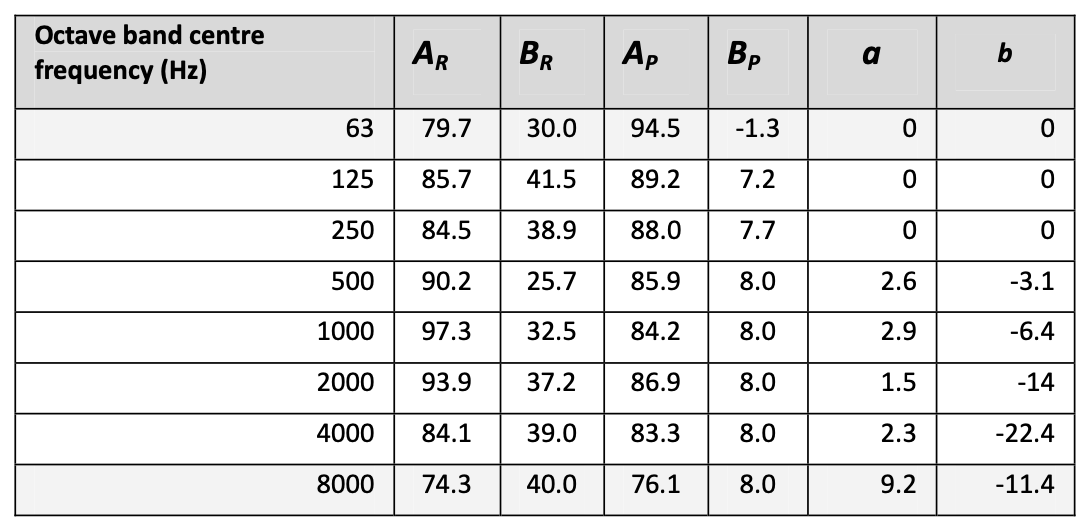
\includegraphics[width=0.75\textwidth]{CNOSSOS/Coefficients for category m=1 vehicles.png}
\end{figure}

\begin{figure}[H]
    \begin{minipage}[c]{.46\linewidth}
        \centering
        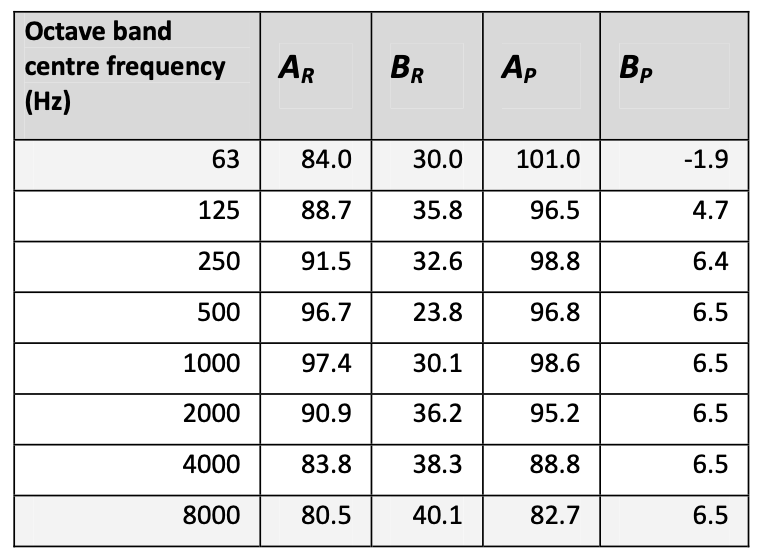
\includegraphics[width=1.1\textwidth]{CNOSSOS/Coefficients for category m=2.png}
        \caption{Coefficients for category m=2}
    \end{minipage}
    \hfill%
    \begin{minipage}[c]{.46\linewidth}
        \centering
        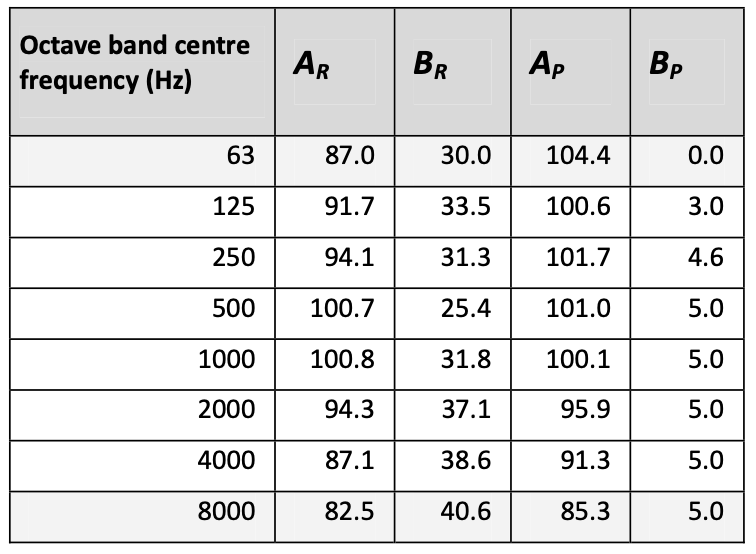
\includegraphics[width=1.1\textwidth]{CNOSSOS/Coefficients for category m=3.png}
        \caption{Coefficients for category m=3}
    \end{minipage}
\end{figure}

\begin{figure}[H]
    \begin{minipage}[c]{.46\linewidth}
        \centering
        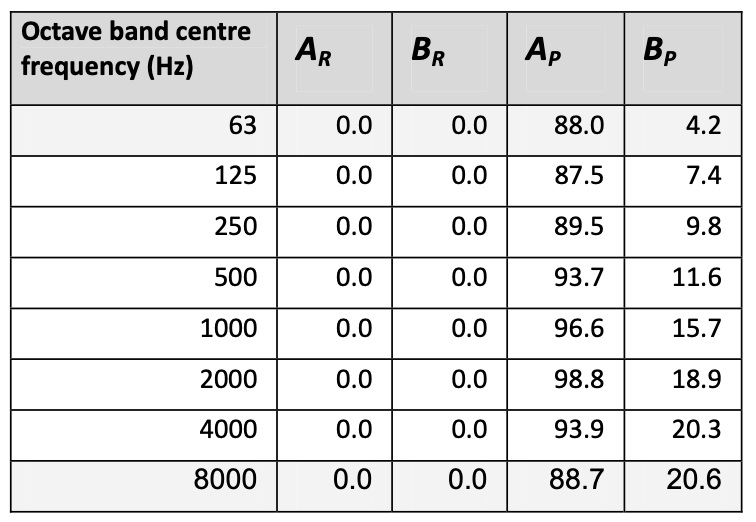
\includegraphics[width=1.1\textwidth]{CNOSSOS/Coefficients for category m=4a vehicles (powered two‐wheelers ≤ 50 cc).png}
        \caption{Coefficients for category m=4a vehicles (powered two‐wheelers $<= 50$ cc)}
    \end{minipage}
    \hfill%
    \begin{minipage}[c]{.46\linewidth}
        \centering
        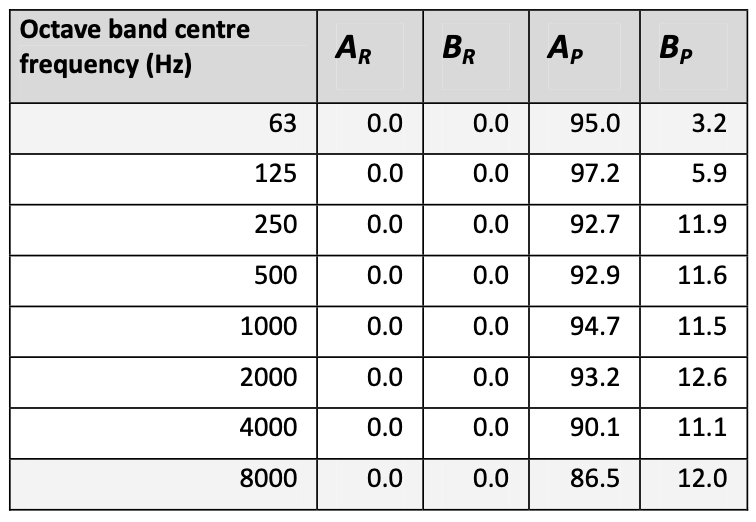
\includegraphics[width=1.1\textwidth]{CNOSSOS/Coefficients for category m=4b vehicles (powered two‐wheelers > 50 cc).png}
        \caption{Coefficients for category m=4b vehicles (powered two‐wheelers $> 50$ cc)}
    \end{minipage}
\end{figure}

\section{Data aggregation of road segments}
\noindent As previously stated, these source emission models calculate the instantaneous sound power level for a single vehicle at a certain location, given the vehicle class, speed, and acceleration. In this section, the instantaneous, single-vehicle sound power level $L_w$ needs to be converted to an equivalent sound pressure level, $L_{e q}$, which is the sound pressure level at a receiver position averaged over a time period in order to determine the noise emission of a vehicle flow on a network connection. Since this aggregating method is introduced in IMAGINE and CNOSSOS model, the analysis below will only consider these 2 models.
 
\noindent To carry out the above-mentioned computation in principle, one should: 
{\color{red} 
\begin{itemize}
    \item Compute the noise impact of each individual vehicle at the receiver point as a function of time while the vehicle passes along the network link; 
    \item Integrate the contribution of each vehicle over time; 
    \item Sum the contribution of all vehicles passing over the network link during a certain time interval; 
    \item Determine the average noise impact of the vehicle flow during a certain time interval
\end{itemize}
}

\noindent {\color{red}This research assumes that the flow of vehicles on the network link with an average speed $v$ at each instant in time is steady, there will be a number of $Q/v$ vehicles per unit length.} $Q$ is the number of vehicles passing per unit time. Instead of integrating over time, one may integrate over the network link's length to get an identical result for the noise impact. The equivalent line source (every sound power per unit length) needs to be calculated first
\begin{equation}
    L_{W,line,eq}=L_{W,0}+10 \lg{\frac{Q}{1000v}}
\end{equation}

\noindent $L_{W,0}$ represents the instantaneous sound power level of a single vehicle. The unit of $L_{W,line,eq}$ is dB per meter, the unit of $Q$ is vehicles per hour, and the unit of $v$ is $km/h$.

\noindent Based on the formula above, the equivalent line sound power levels for all different vehicles can be summed, and the average equivalent line sound power level of multiple $L_{W,eq,i}$ values is calculated by:
\begin{equation}
    L_{W,eq,avg}=10 \lg{\frac{1}{N} \sum_{i=1}^N 10^{L_{W,eq,i}/10 }}
\end{equation}
\noindent Where $L_{W,eq,i}$ represents the $N$ separate equivalent line sound power levels.


\section{{\color{red} Discussion}}

\subsection{Assumption for choosing the parameter of the IMAGINE model and the {\color{red} CNOSSOS} model}
\noindent From the introduction of the IMAGINE model and the CNOSSOS model, it could be seen that the calculation of the noise emission is related to 3rd octave bands, which cannot be acquired from Pneuma dataset. Therefore, based on the range of all the parameters of these 2 models, maximum value and minimum value are calculated, which is shown in Figure \ref{fig:11}.
\begin{figure}[h]
\begin{subfigure}{.5\textwidth}
  \centering
  % include first image
  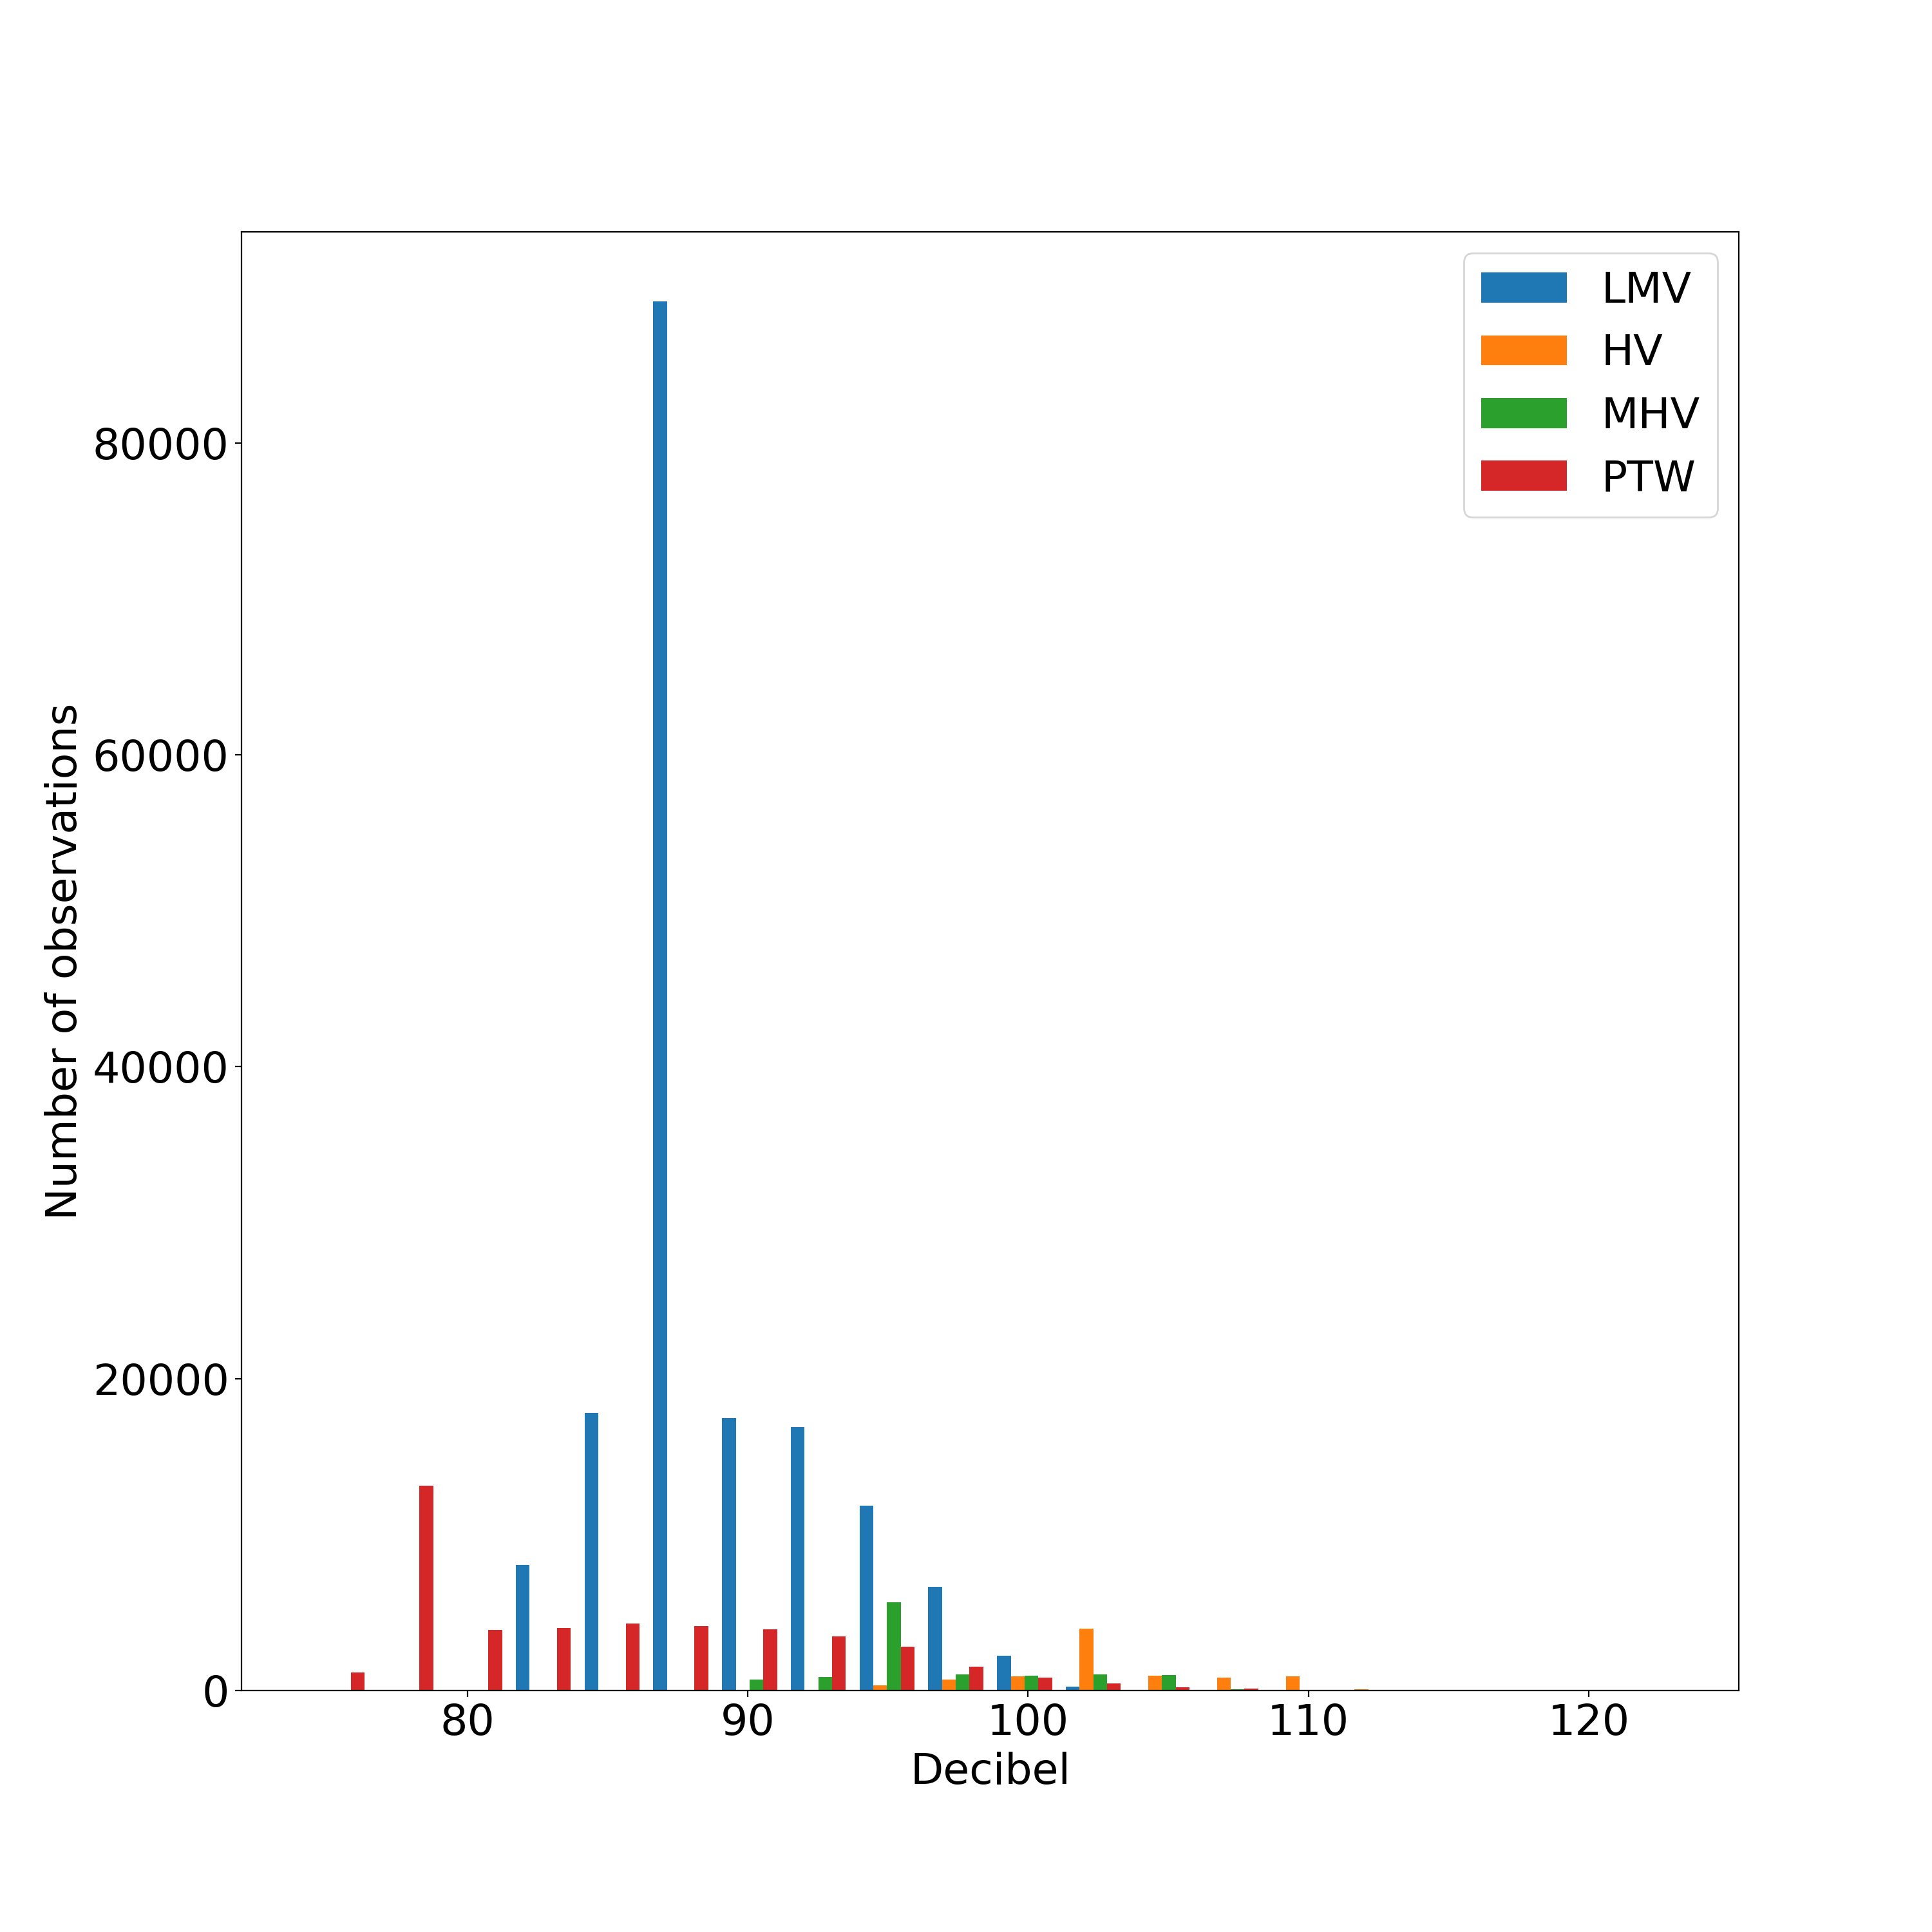
\includegraphics[width=.8\linewidth]{IMAGINE model max.png}  
  \caption{IMAGINE model (implementing the max parameters in the range)}
  \label{fig:sub-first}
\end{subfigure}
\begin{subfigure}{.5\textwidth}
  \centering
  % include second image
  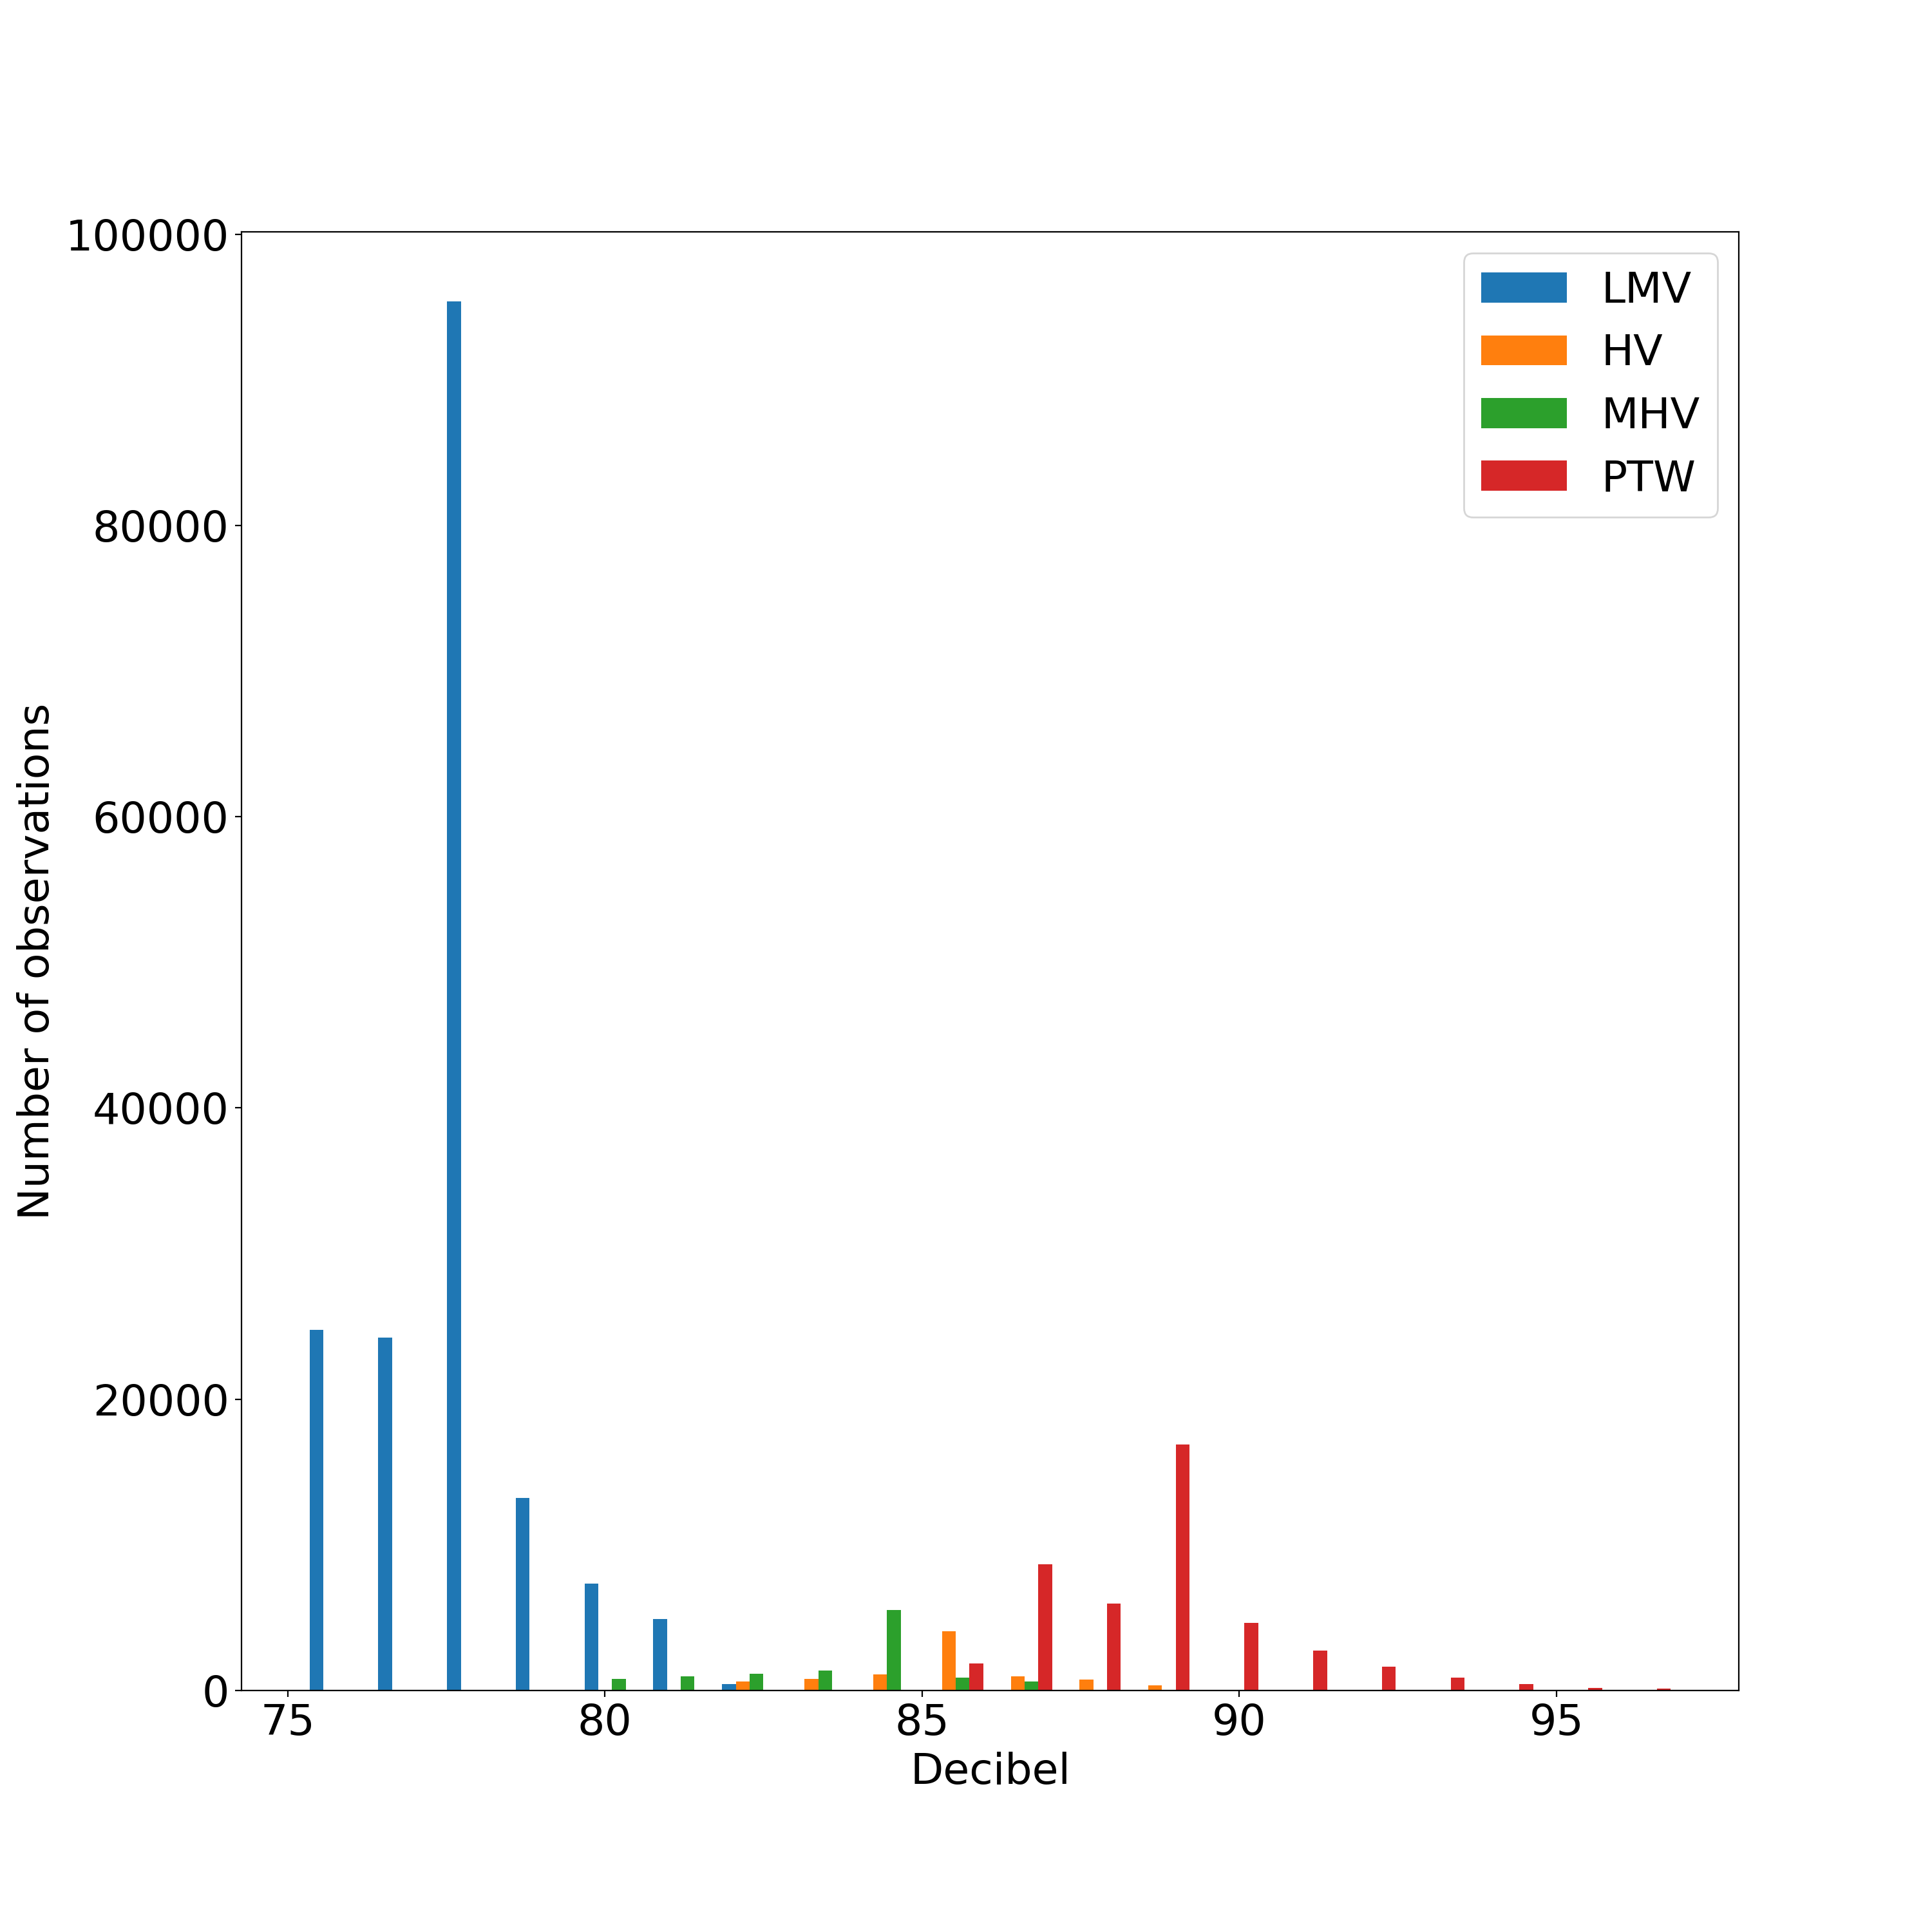
\includegraphics[width=.8\linewidth]{IMAGINE model min.png}  
  \caption{IMAGINE model (implementing the min parameters in the range)}
  \label{fig:sub-second}
\end{subfigure}

\newline

\begin{subfigure}{.5\textwidth}
  \centering
  % include third image
  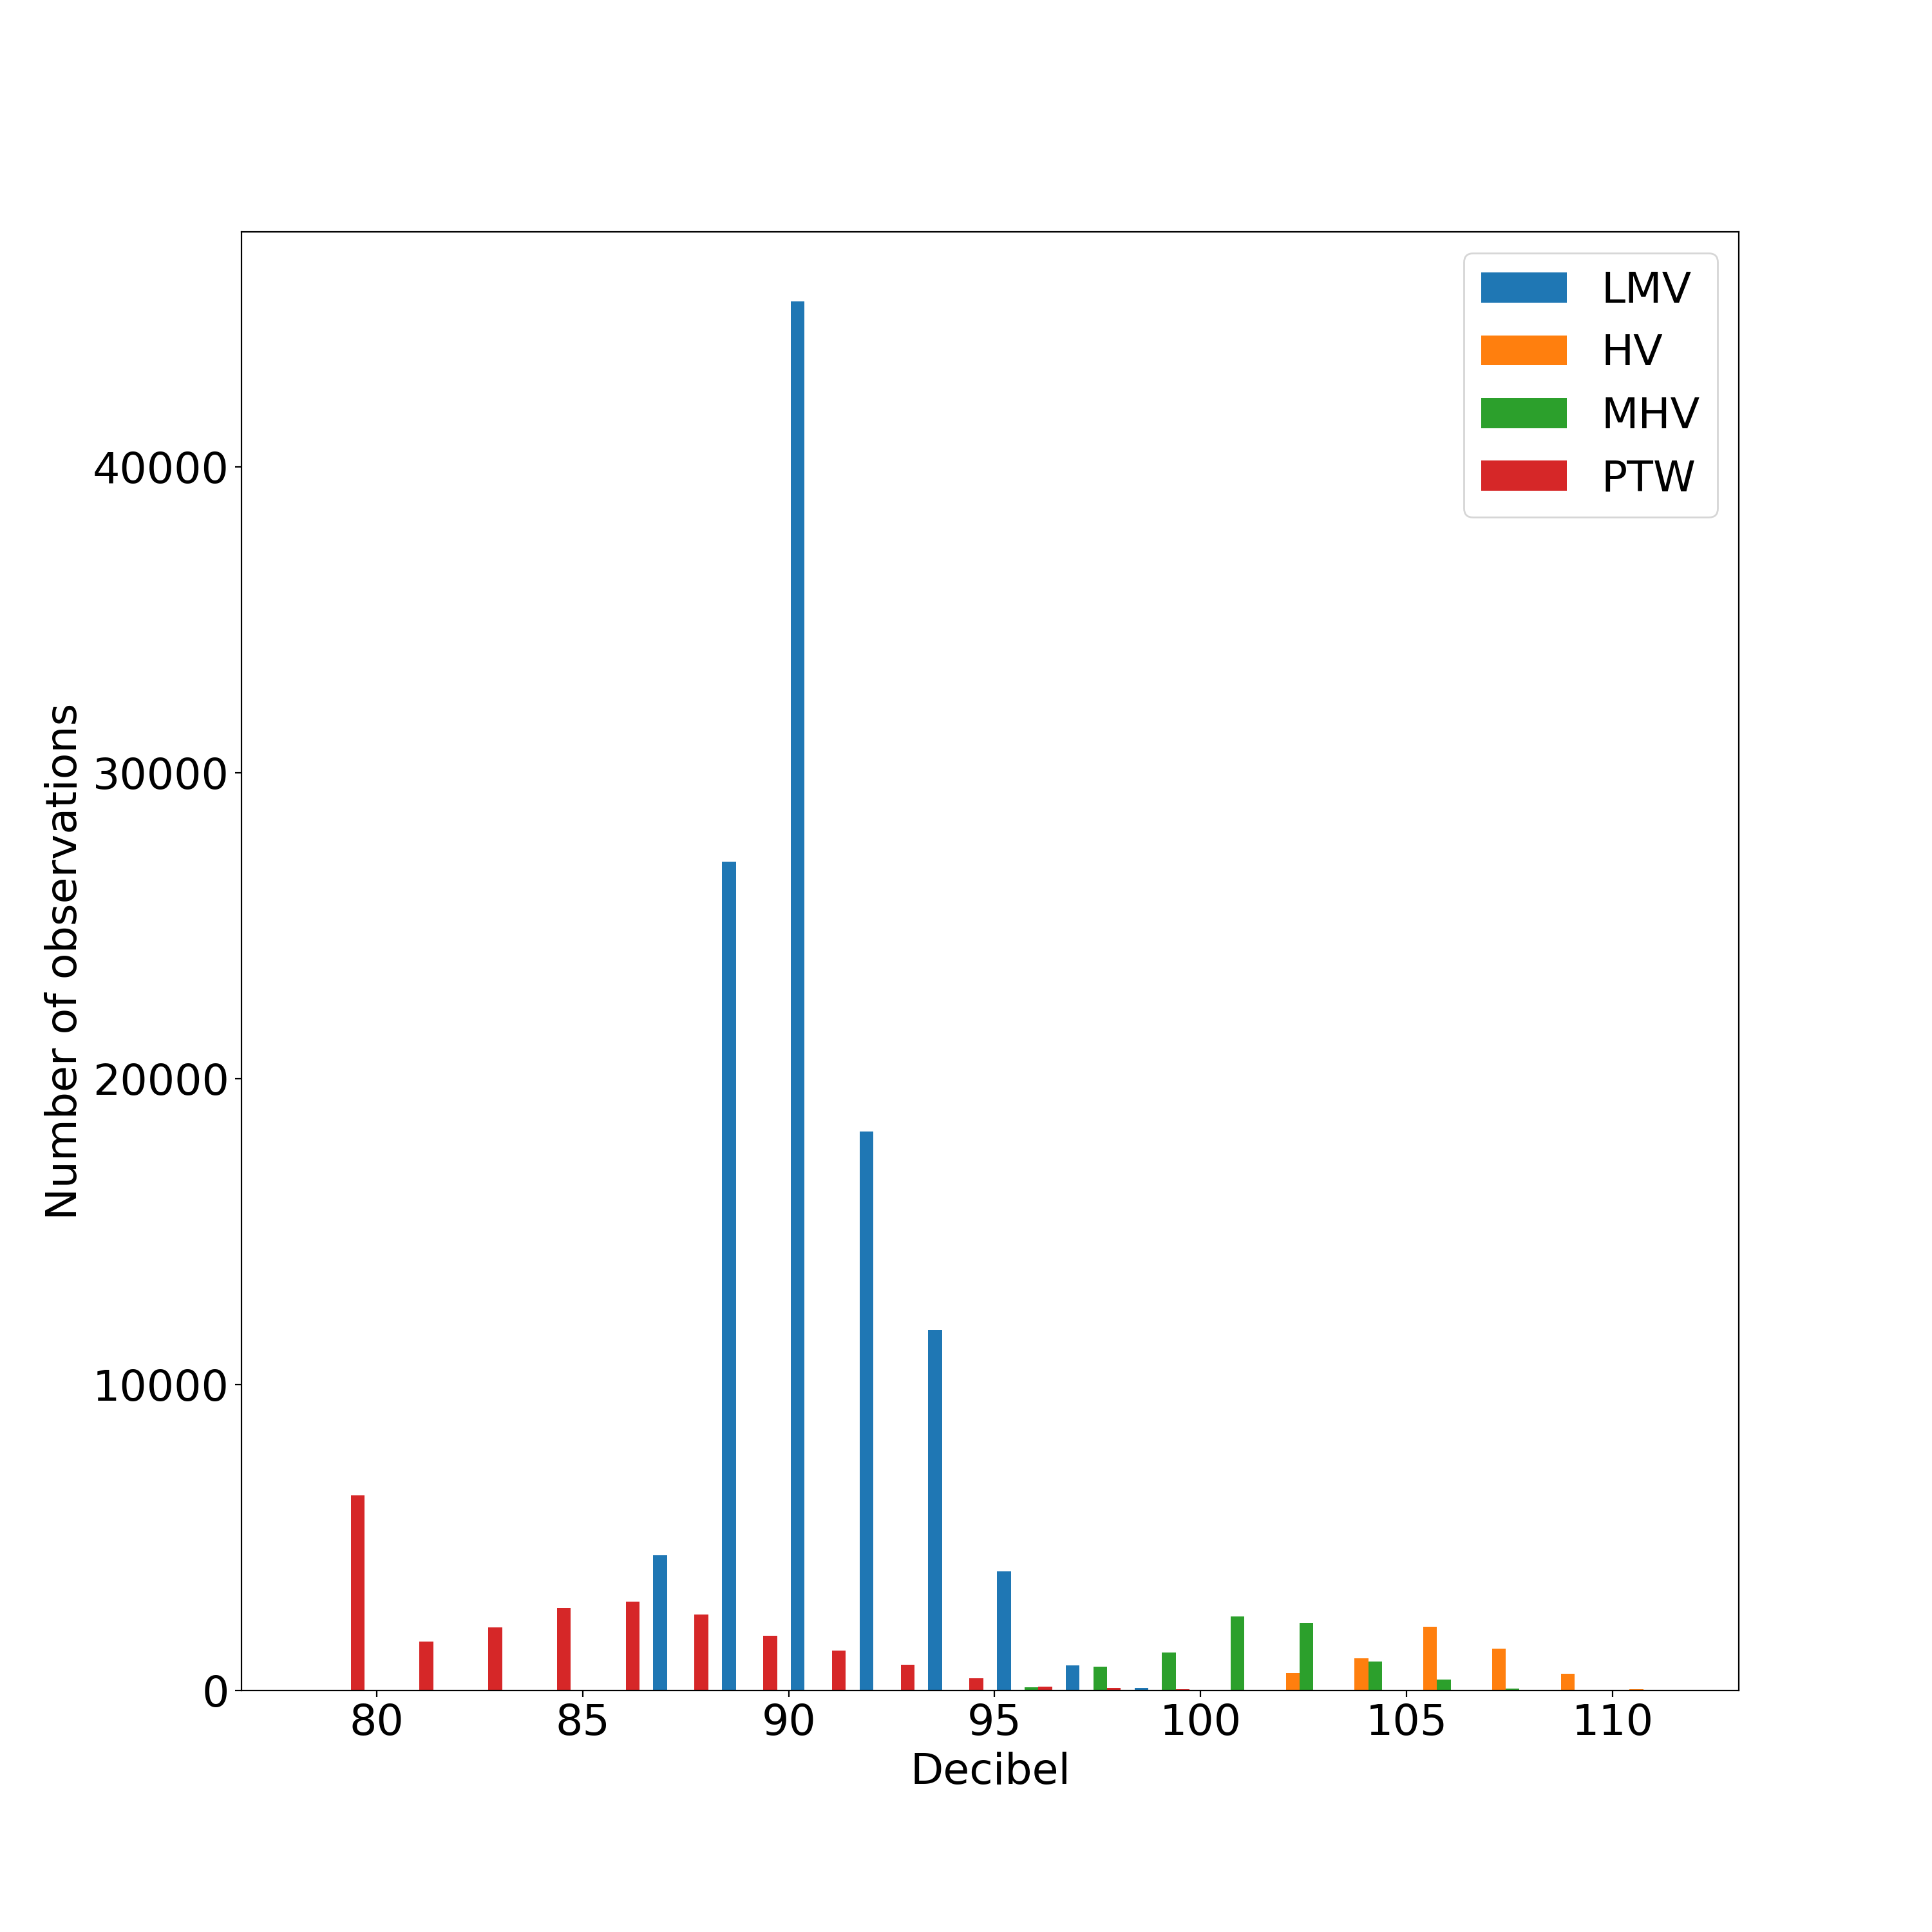
\includegraphics[width=.8\linewidth]{CNOSSOS model max.png}  
  \caption{CNOSSOS model (implementing the max parameters in the range)}
  \label{fig:sub-third}
\end{subfigure}
\begin{subfigure}{.5\textwidth}
  \centering
  % include fourth image
  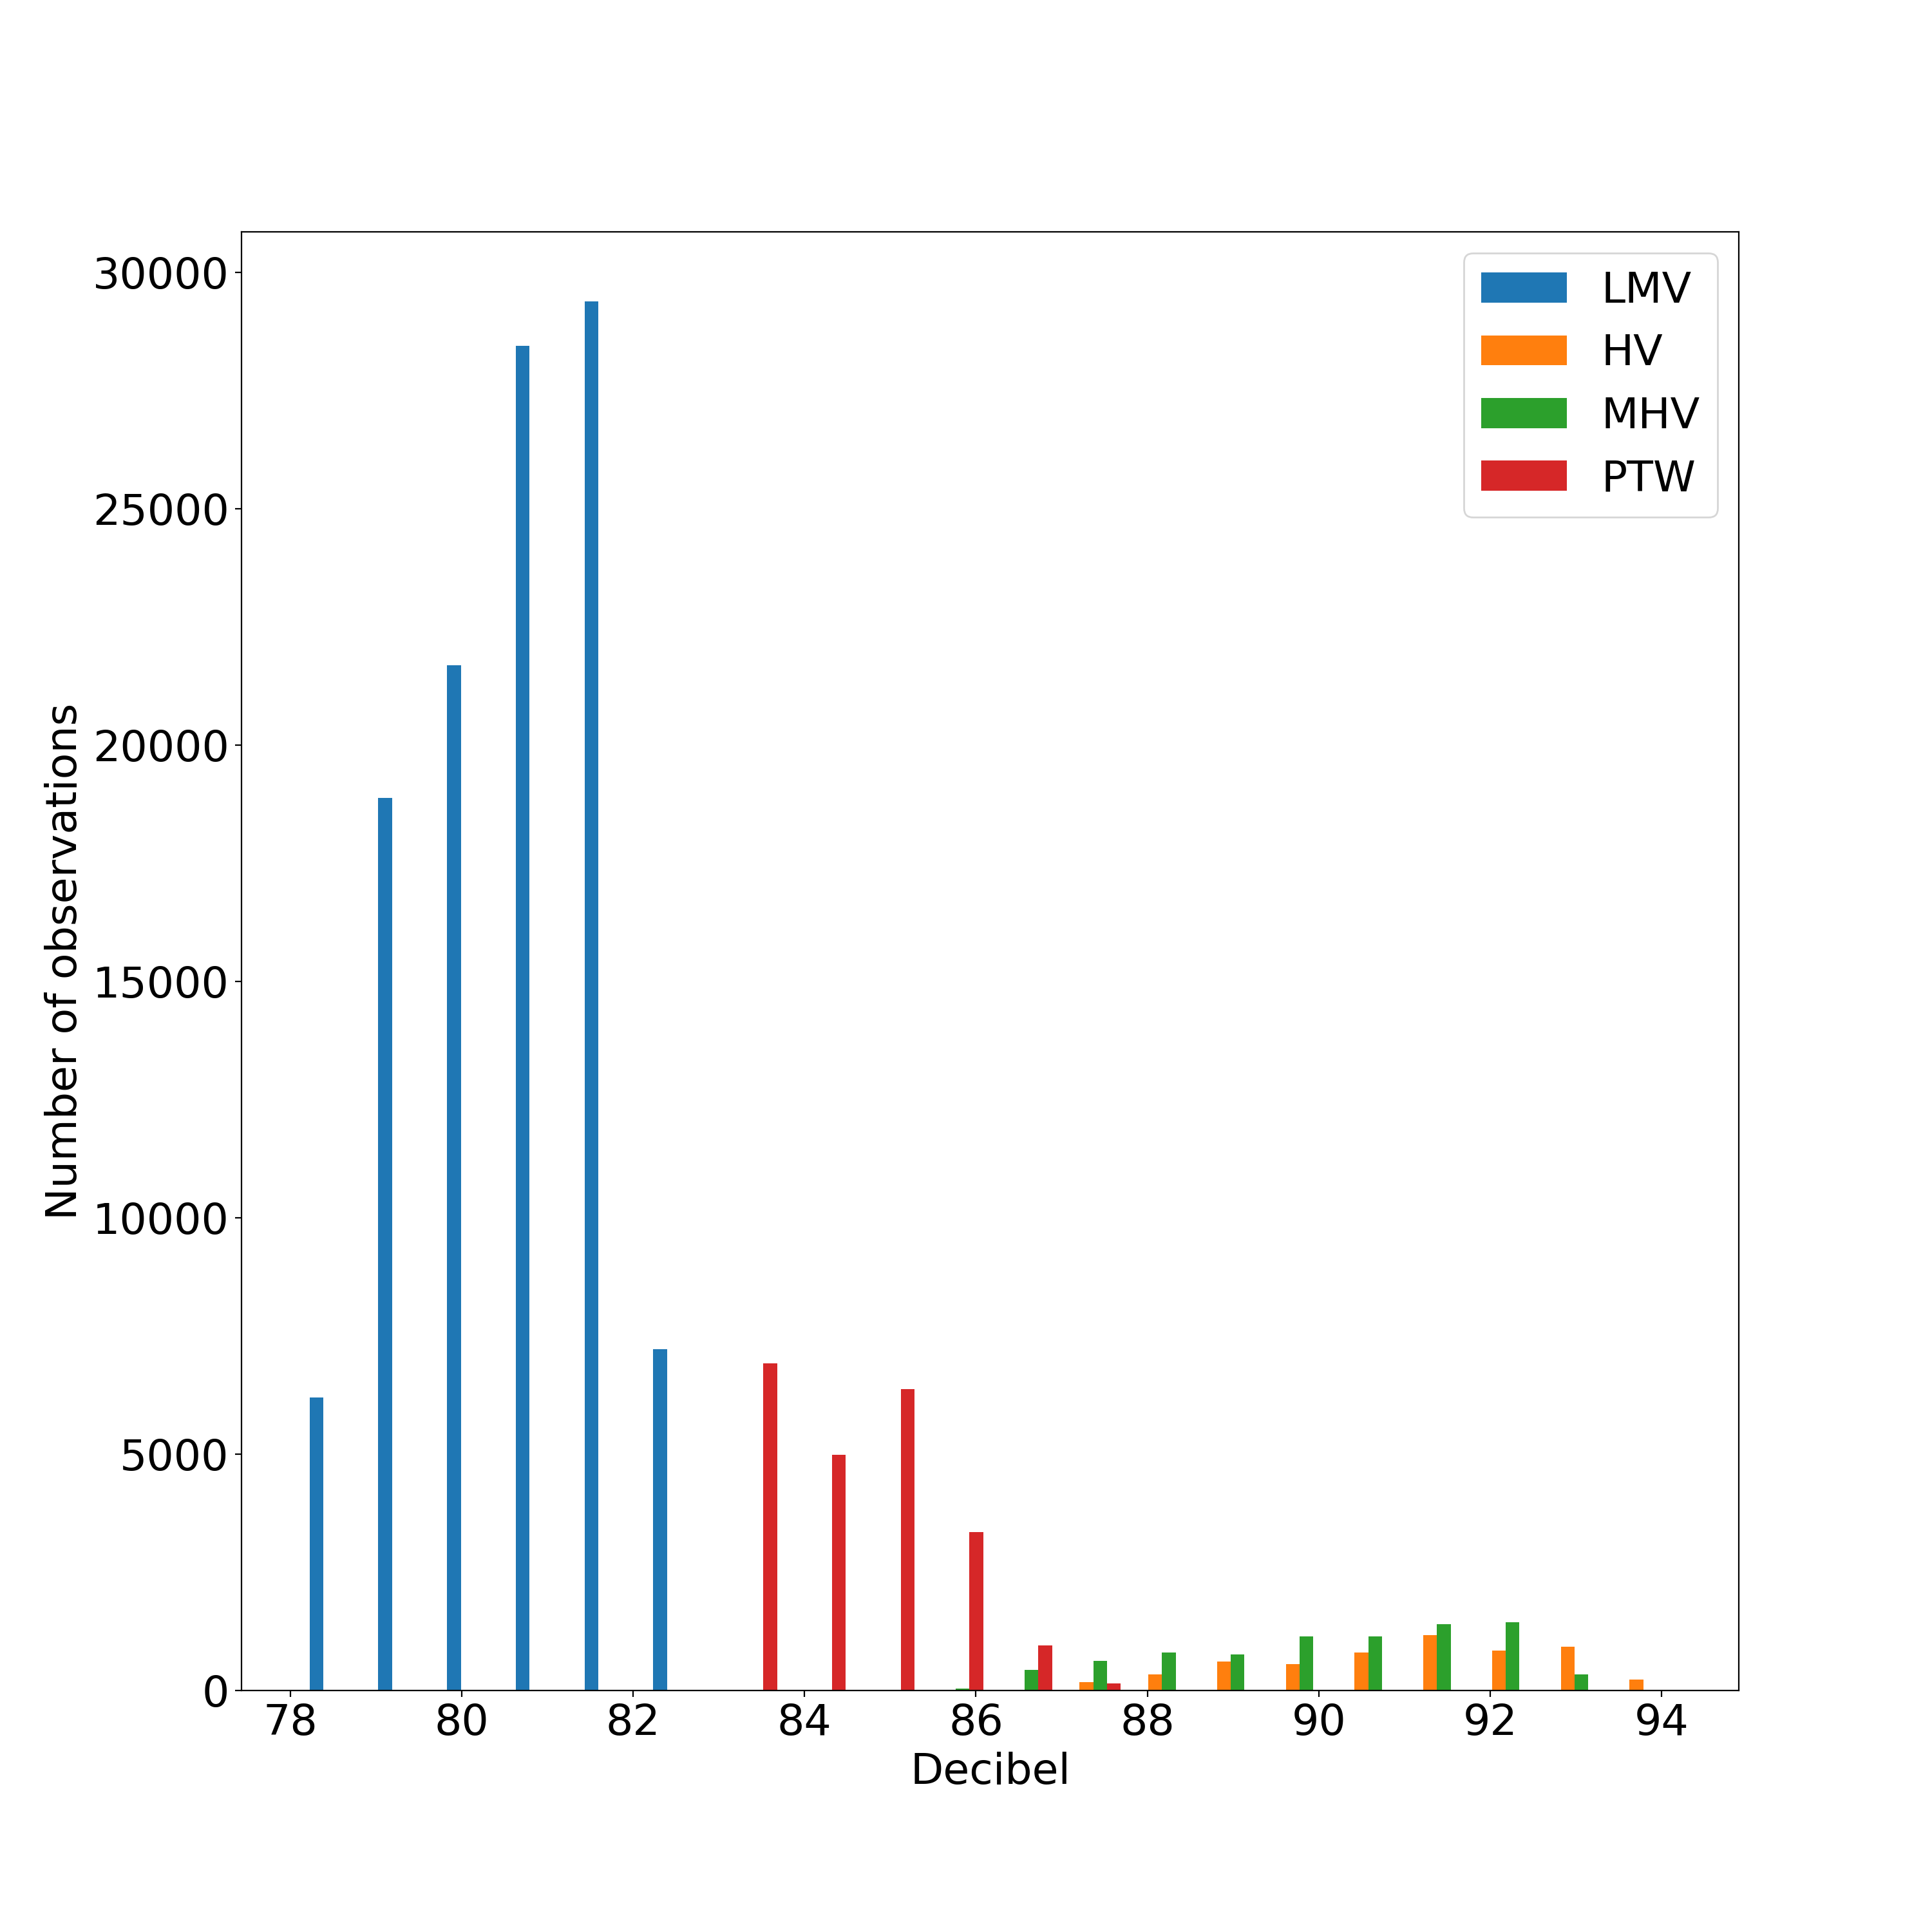
\includegraphics[width=.8\linewidth]{CNOSSOS model min.png}  
  \caption{CNOSSOS model (implementing the min parameters in the range)}
  \label{fig:sub-fourth}
\end{subfigure}
\caption{The noise distribution of IMAGINE and CNOSSOS model based on the different parameters}
\label{fig:11}
\end{figure}

\noindent Since no ground truth can be acquired in this research, the minimum value is chosen based on the common sense, which is the motorcycle will produce higher noise than the car because of its poor noise reduction performance, in the further study, the ground truth data should be measured so that the best model and the best parameters can be acquired.
\subsection{Analysis of the noise emission distribution}
\noindent In this section, three models are analyzed by plotting the noise emission distribution by vehicle types based on a specific zone in Athens.

\noindent Firstly, the NMPB model is implemented. Since the NMPB model only considers the speed over 5 km/h, the vehicle whose speed is lower than 5km/h will not be analyzed here. In this model, there are only 2 types of vehicle: light vehicles(motorcycle, taxi, car and medium heavy vehicle) and heavy vehicle(bus and heavy vehicle). From Figure \ref{NMPB model}, it can be observed that in the heavy vehicle, the range of the noise emission is higher, which is from 74dB to 83dB, while the range of the noise emission in the light vehicle is from 62dB to 78dB.

\begin{figure}[h]
    \begin{center}
        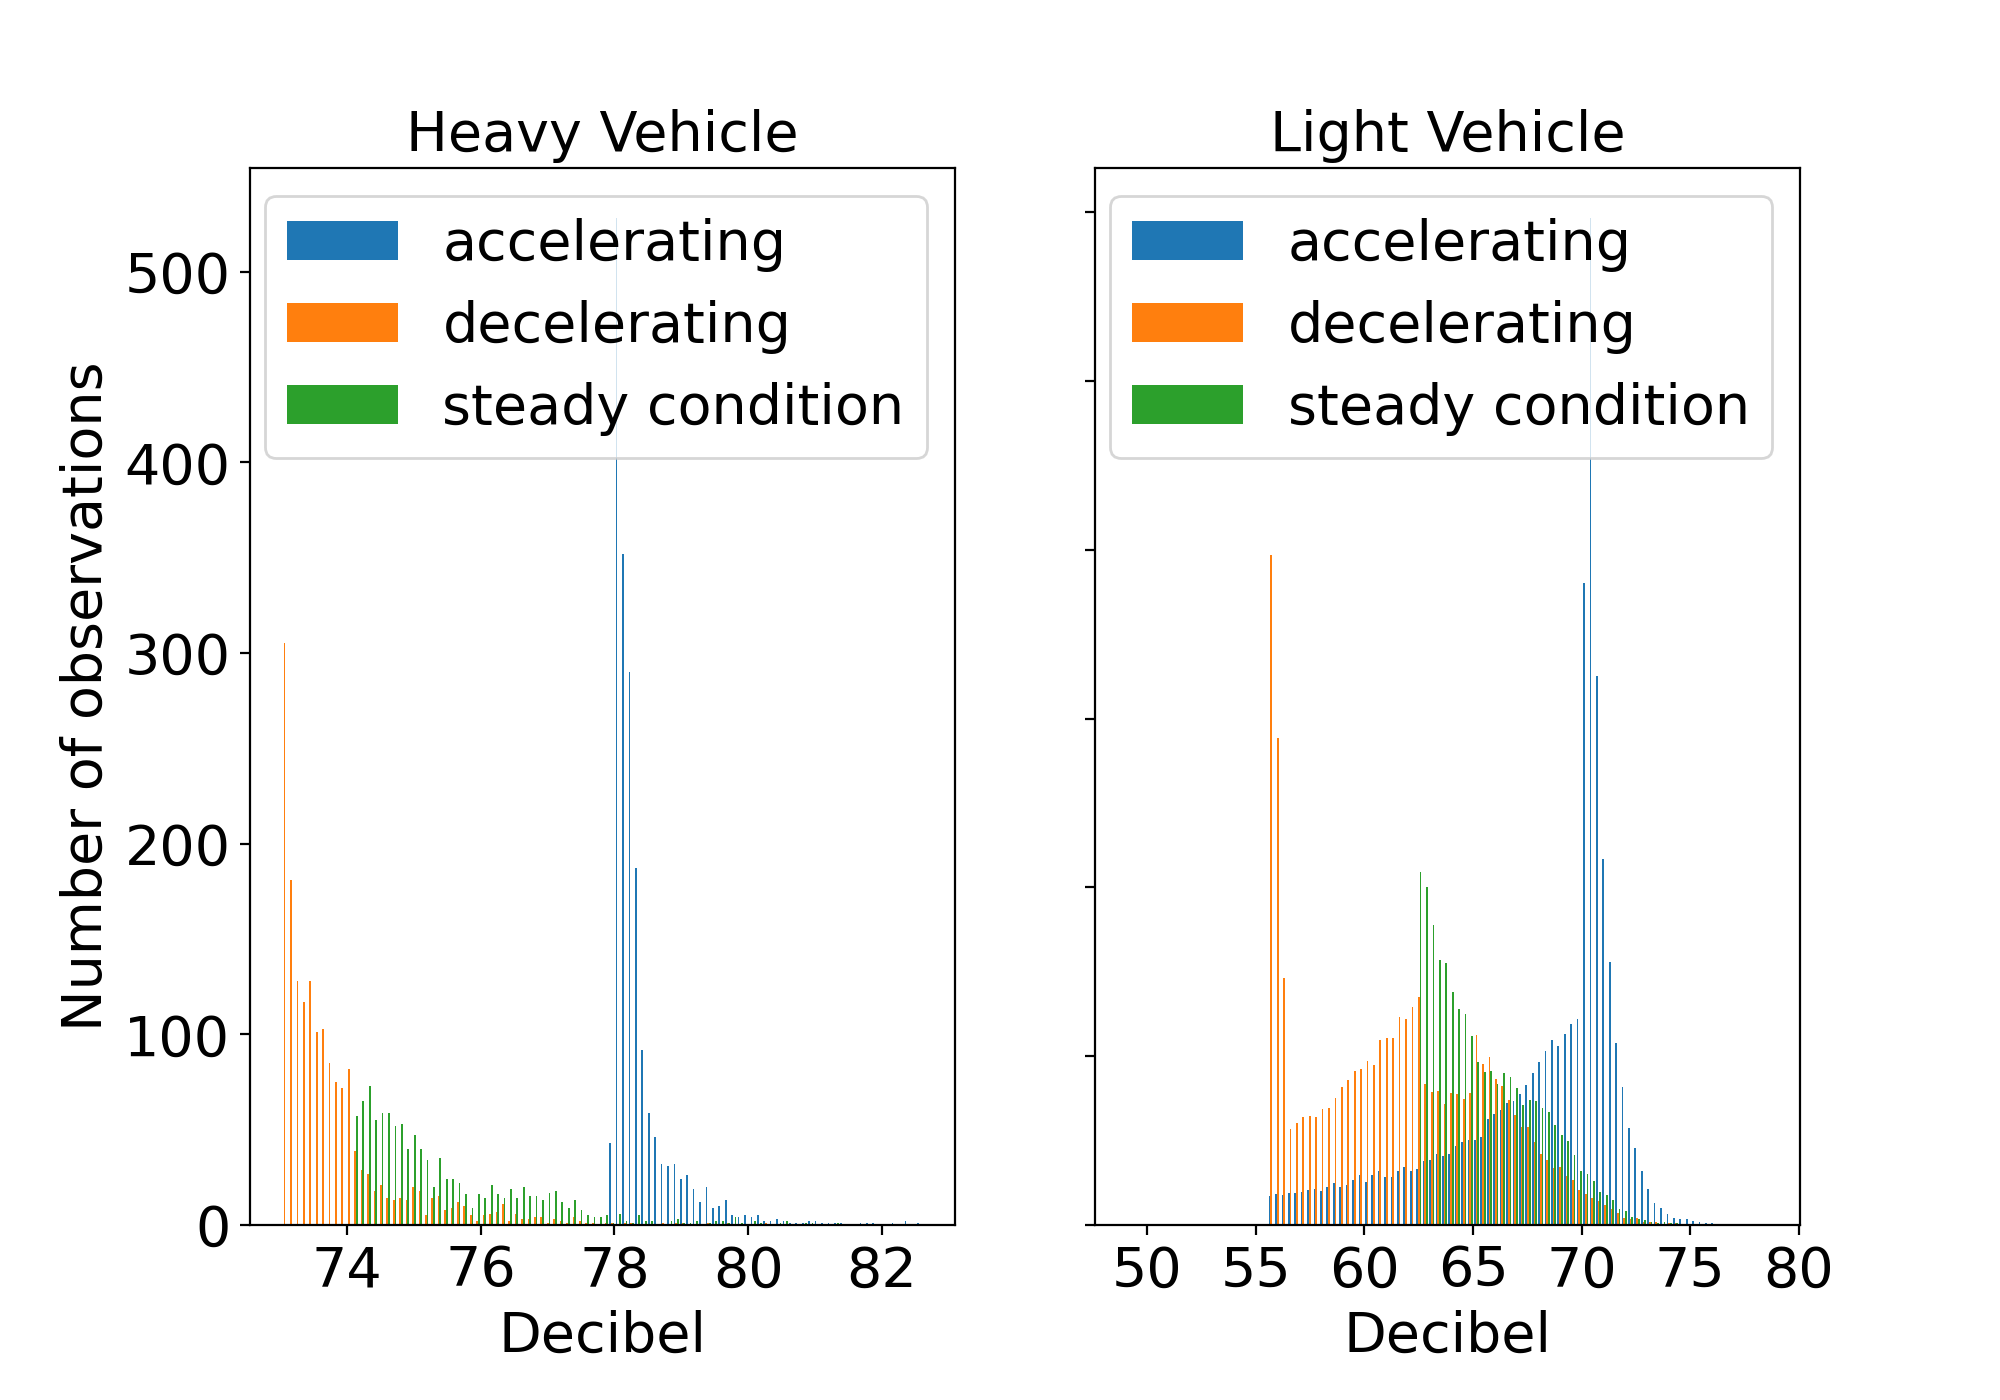
\includegraphics[width=0.8\textwidth]{NMPB model.png}
        \caption{NMPB model}
        \label{NMPB model}
    \end{center}
\end{figure}

\noindent Besides, in this graph, 3 clusters could be observed in both categories, because NMPB model considers both the speed and the acceleration state of the vehicle, if the vehicle is regarded as accelerating, it will create higher noise emission, however, in the other acceleration state(steady state and decelerating state), it will create fewer noise emission. On the other hand, with the increasing of the speed, the vehicle will also create higher noise mission.


\noindent Secondly, the IMAGINE model is implemented. Since the parameters of PNC and RNC is decided by the 3rd octave bands, but it is impossible to acquire the 3rd octave bands of each vehicle in the Pneuma dataset. Therefore, this research implements the minimum of the parameters of PNC and RNC in order to find out the range of noise emission distribution in each category.

\noindent The minimum noise emission is calculated in the picture below, it could be seen from Figure \ref{fig:11} that the noise emission range of all vehicles is from 73dB to 96dB. It is easily found  that there are some high bars in specific noise emission area, because the speed of vehicle is 0 in these areas. If the data of static vehicle is removed, from Figure \ref{IMAGINE model}, the distribution of each type of vehicle follows the sum of several normal distributions. These phenomenons could be explained as following reasons:

\begin{figure}[h]
    \begin{center}
        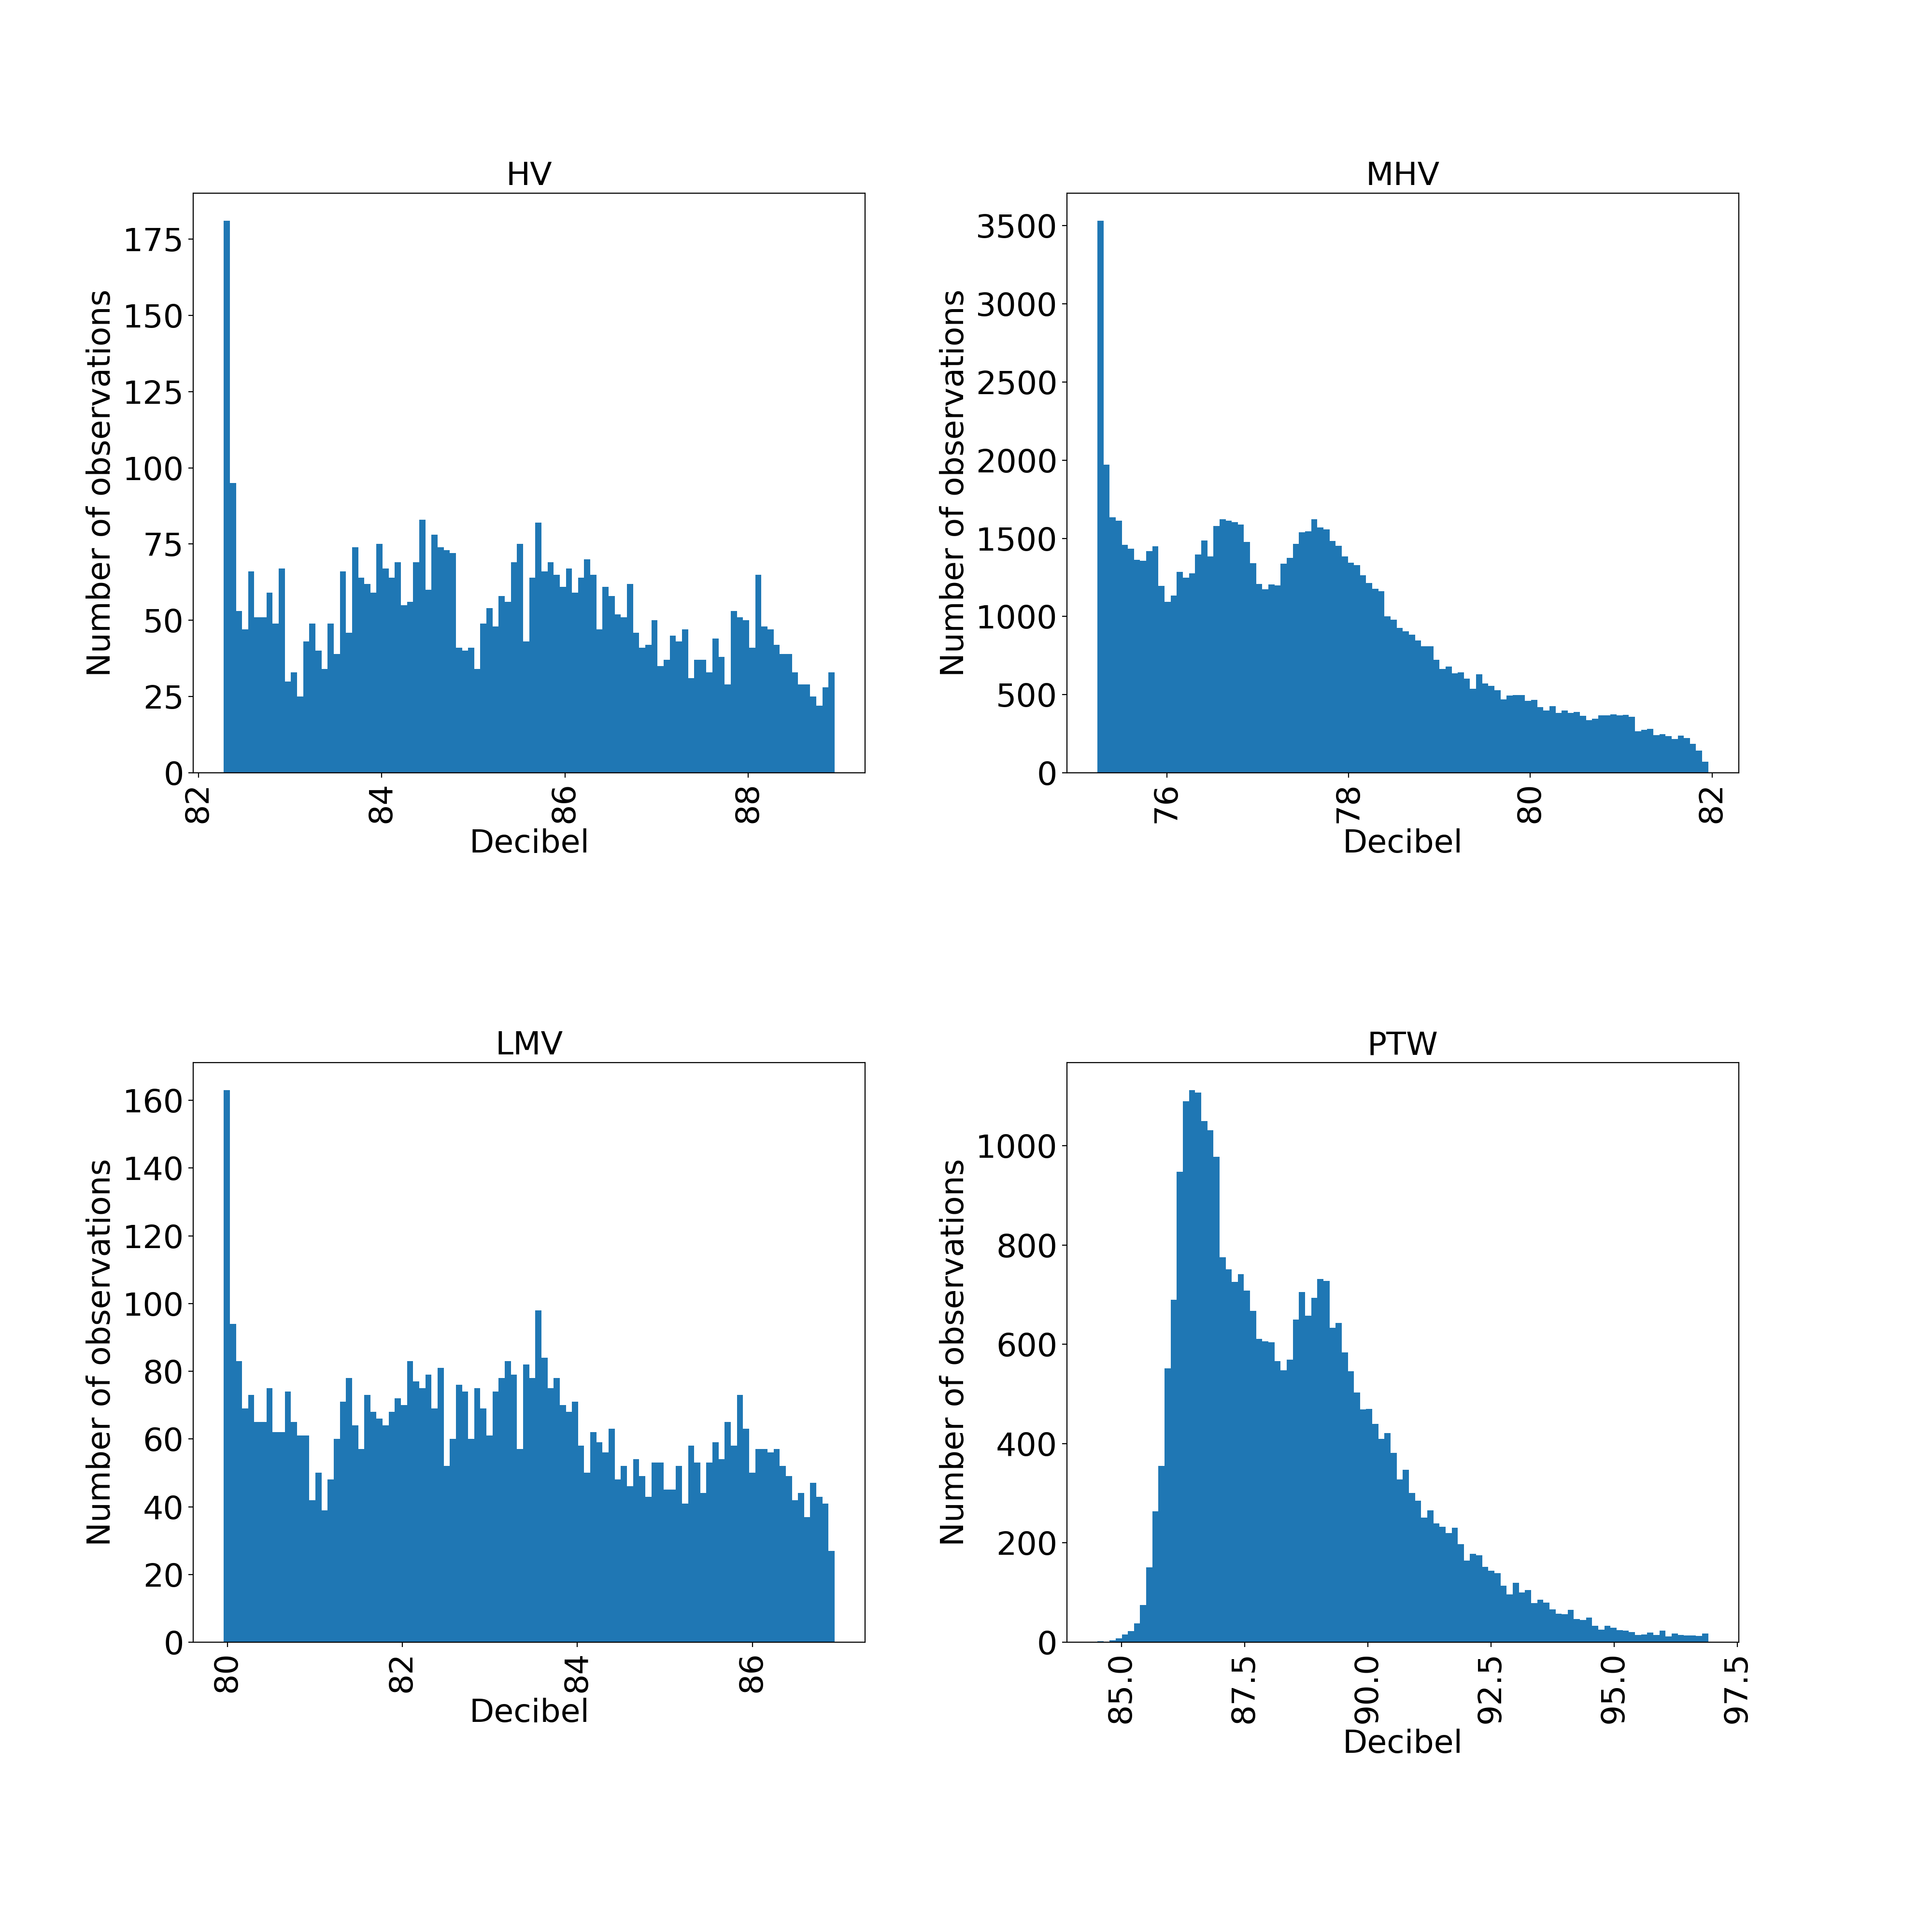
\includegraphics[width=14cm]{IMAGINE model.png}
        \caption{IMAGINE model}
        \label{IMAGINE model}
    \end{center}
\end{figure}

\noindent 1. If the vehicle is not moving, it can still create noise. This could happen because the IMAGINE model assumes that even when the vehicle is not moving, the engine is still working, therefore, the propulsion noise component is not zero.


\noindent 2. Since the IMAGINE model takes into account the extent of acceleration rather than only consider the state of the vehicle, the distribution of the noise emission is more uniform than the NMPB model.

\noindent 3. it is counter intuition that some vehicles can produce fewer noise than the vehicle whose speed is zero.  Since the IMAGINE model neglects the influence of the tire slip during braking or acceleration and corrects only propulsion noise source, and it also assumes that the decelerating could reduce the noise emission compare to the static condition. Therefore, it is possible that some vehicles can produce fewer noise than the vehicle whose speed is zero based on the assumption of IMAGINE model.

\noindent Finally, the CNOSSOS model is implemented. Since the distance to the nearest intersection are required to be calculated, based on the given dataset, only the noise emission of the vehicle in the road $Αλεξάνδρας$ could be calculated. The distribution of 4 categories is shown in Figure \ref{CNOSSOS model}. Based on this graph, several phenomenons could be found:

\begin{figure}[h]
    \begin{center}
        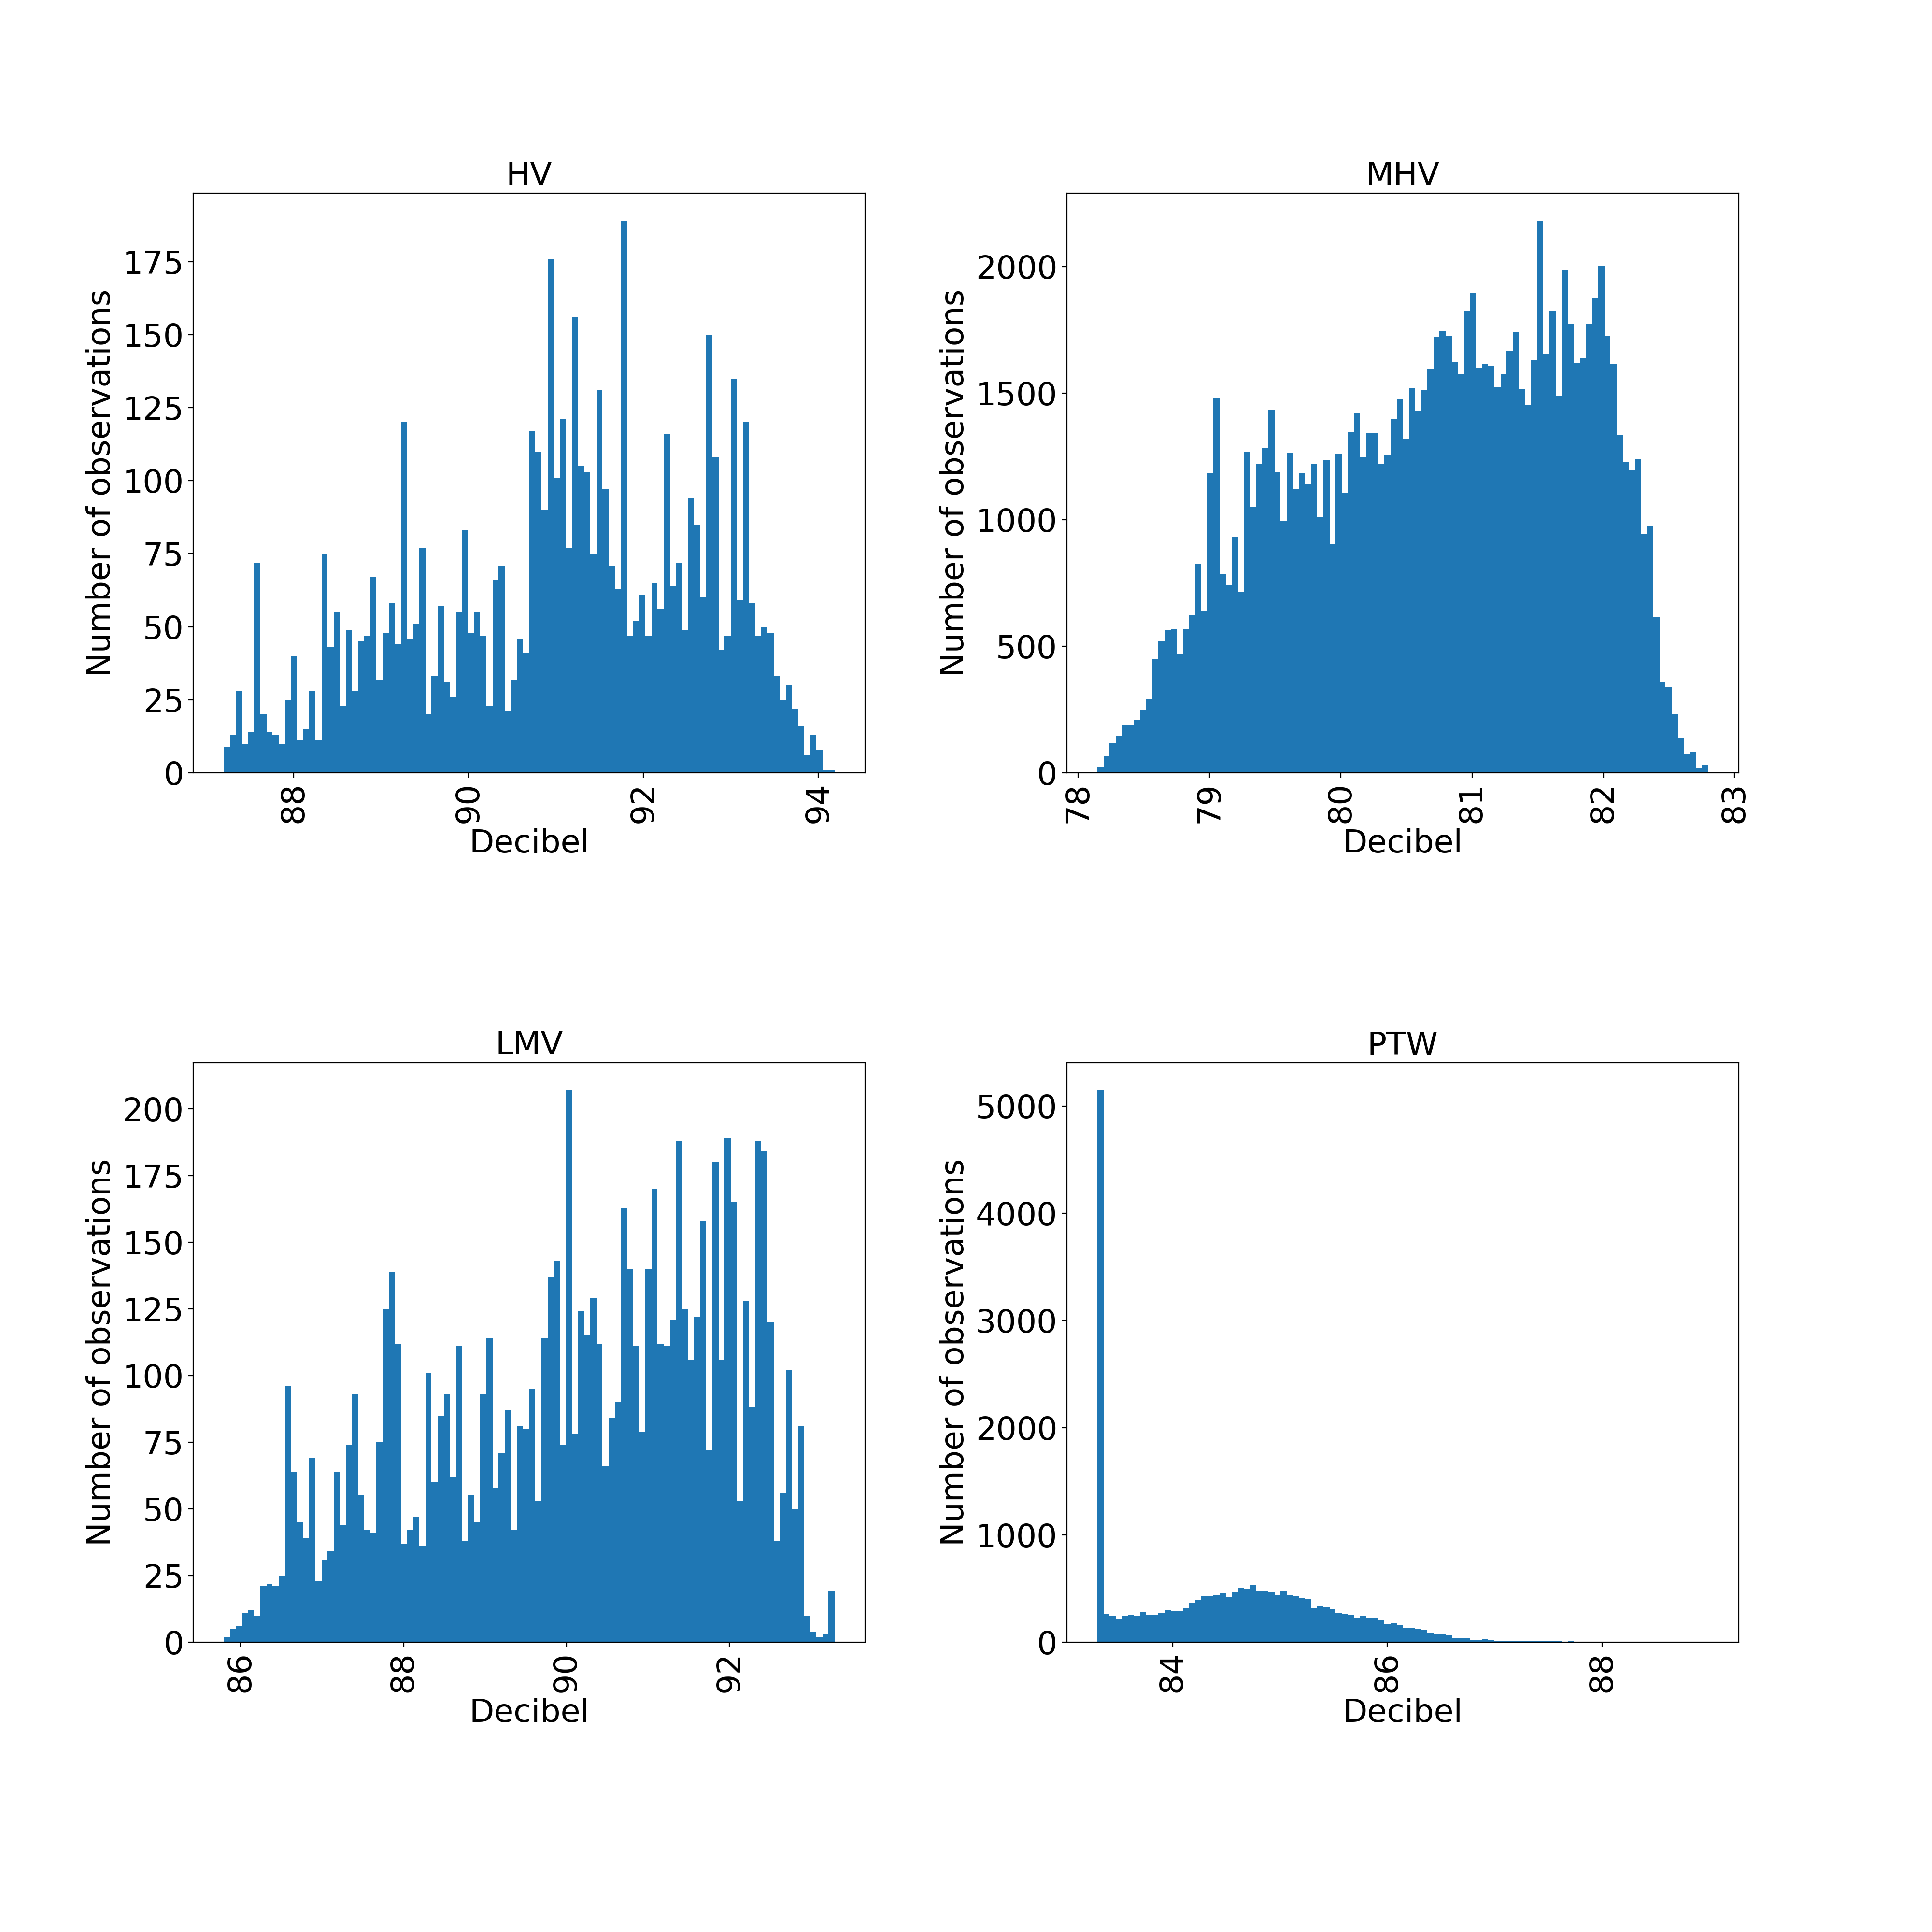
\includegraphics[width=14cm]{CNOSSOS model.png} 
        \caption{CNOSSOS model}
        \label{CNOSSOS model}
    \end{center}
\end{figure}


\noindent 1. Compared to the IMAGINE model, no high bar could be found in the distribution, because the acceleration correction factor is related to the distance to the nearest intersection, if several vehicles are not moving but located in different places, then the noise emission of these vehicles are different.

\noindent 2. It is easy to be found that heavy vehicles(bus and heavy vehicle) and medium heavy vehicles could produce higher noise emission than the motorcycle than the light vehicles(car and taxi).

\newpage

\subsection{Comparison between 3 models}

\noindent The Figure \ref{Comparisons between 3 models} shows the noise emission distribution from 3 models sorted by different categories, several phenomenon could be found:
\begin{figure}[h]
    \begin{center}
        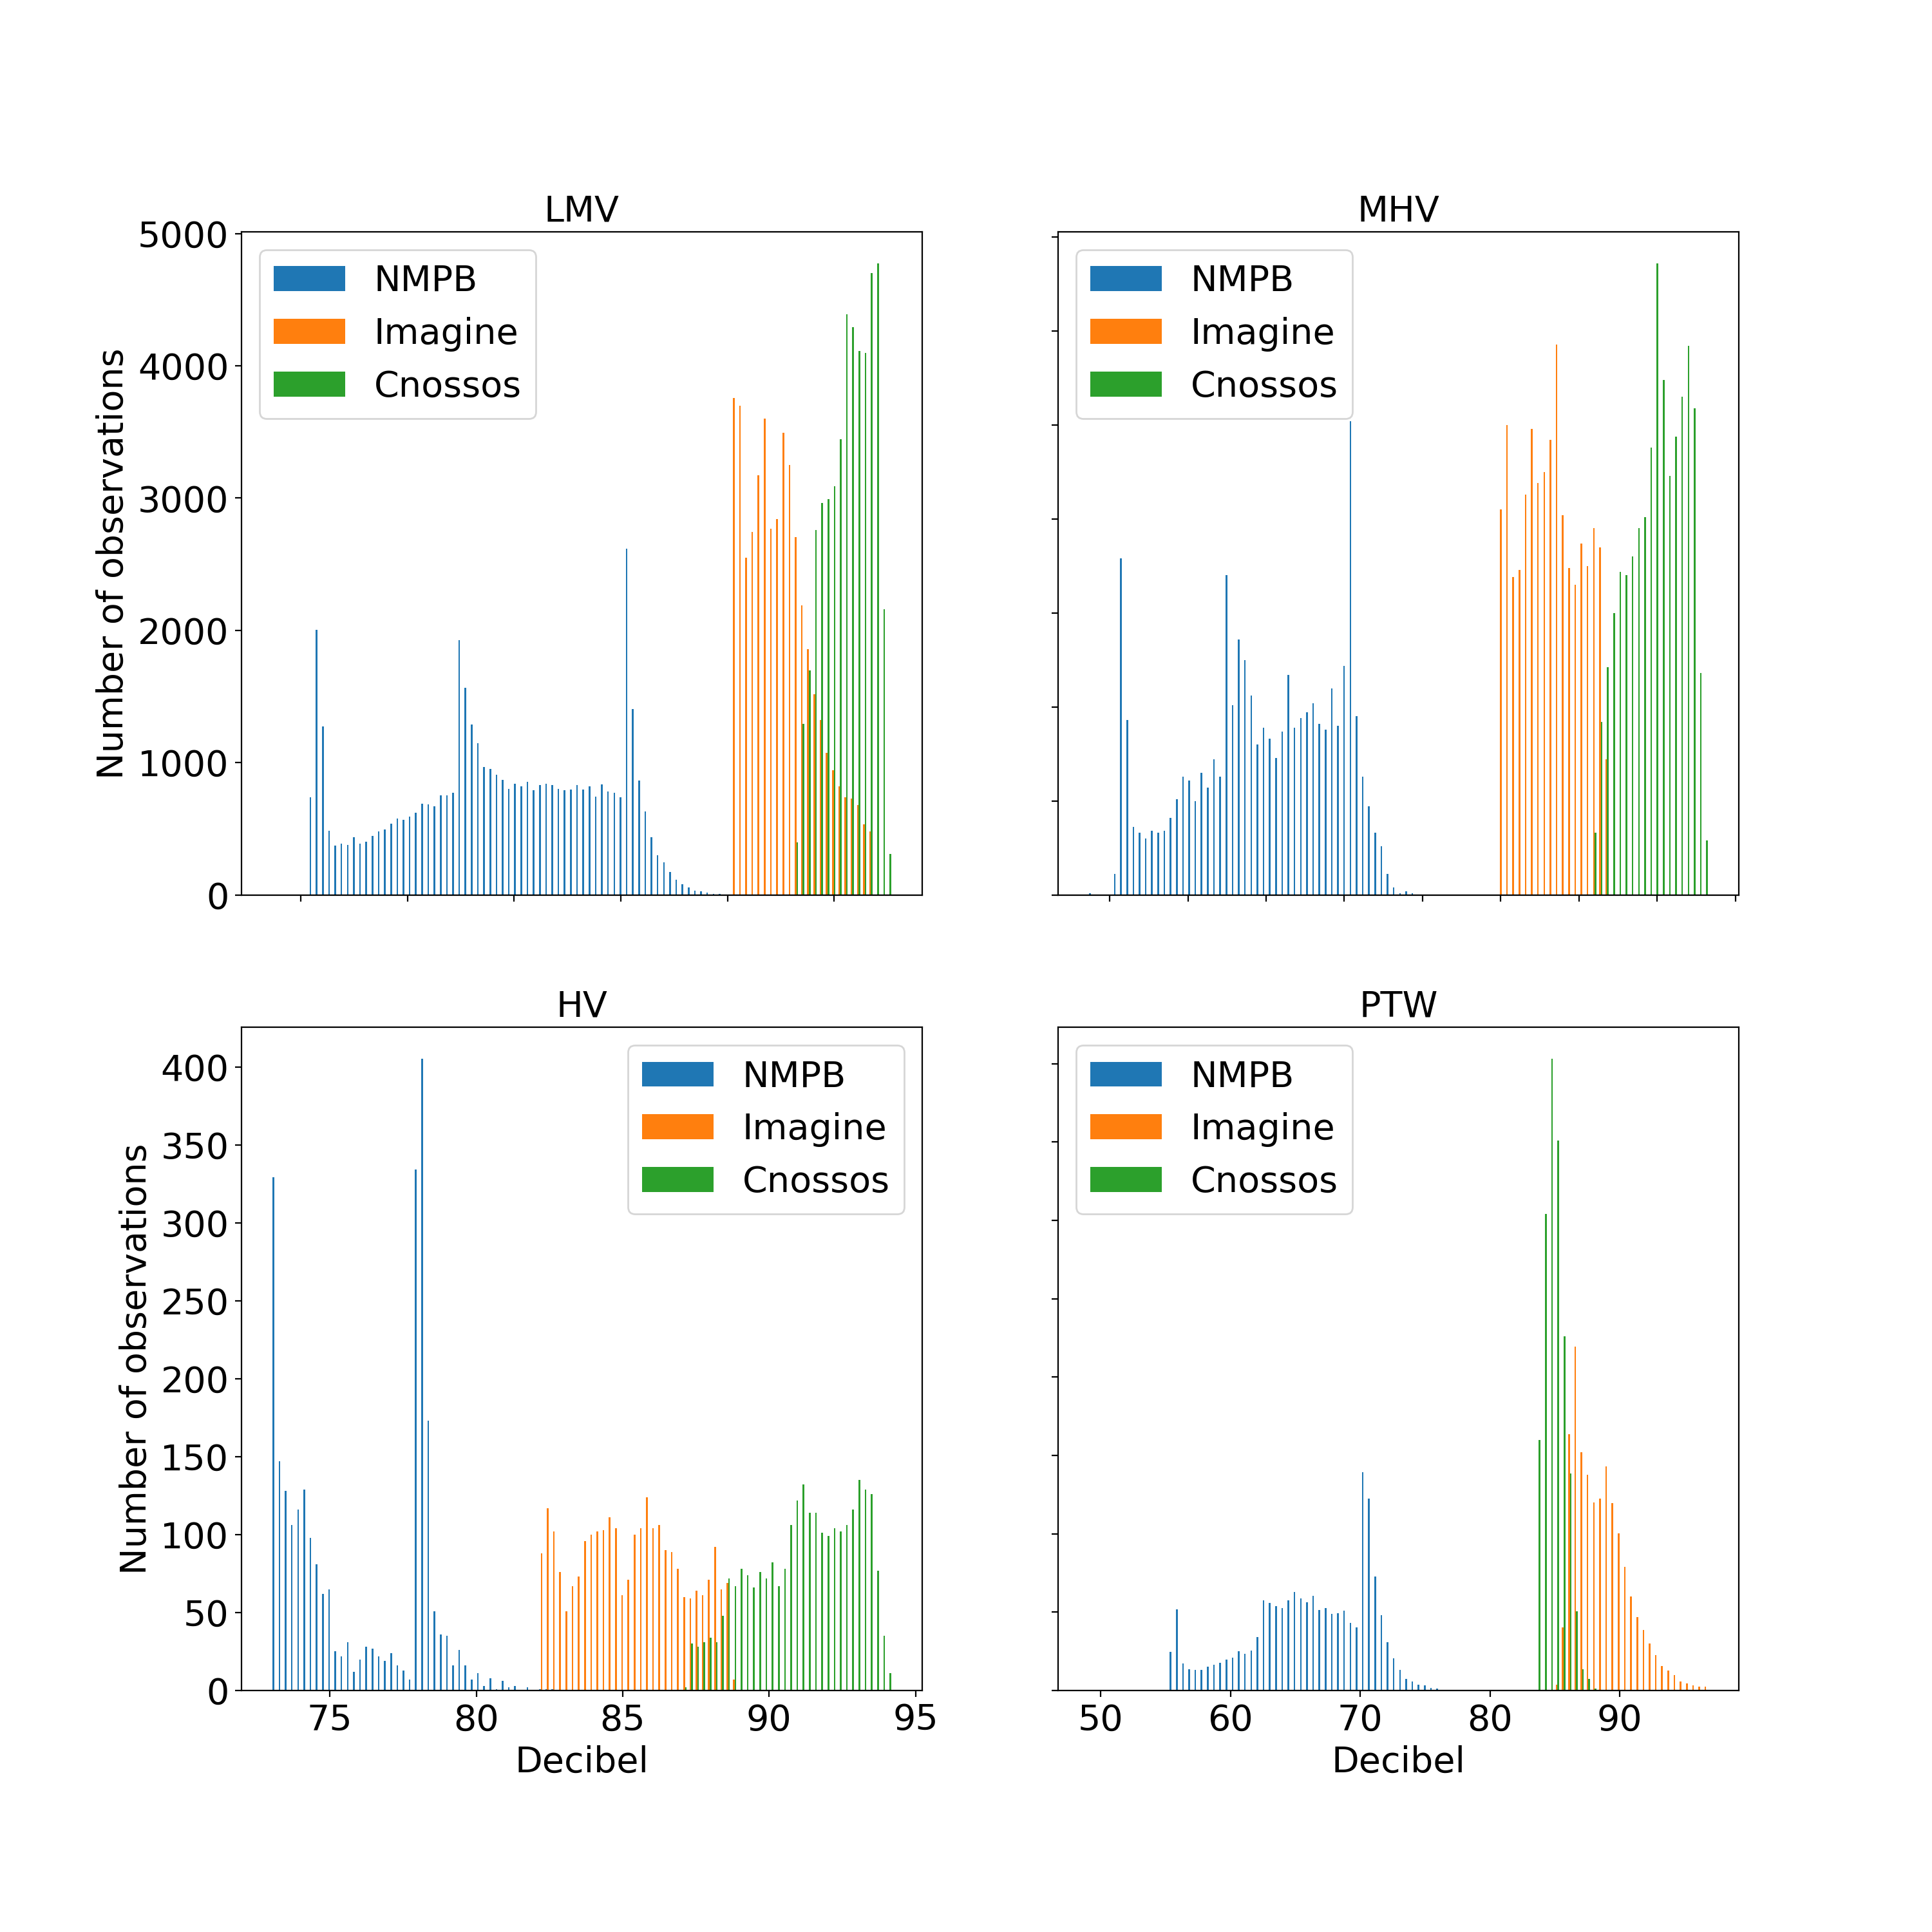
\includegraphics[width=14cm]{Comparisons between 3 models.png}
        \caption{Comparisons between 3 models}
        \label{Comparisons between 3 models}
    \end{center}
\end{figure}

\noindent 1. Except for the noise emission distribution of motorcycle, the CNOSSOS model will acquire higher value than the IMAGINE model than the NMPB model. The reason why the CNOSSOS model get higher noise emission than IMAGINE model is that the correction factor of acceleration is higher.

\noindent 2. Since the CNOSSOS model does not consider the acceleration correction factor for the motorcycle category, the value of CNOSSOS model is lower than IMAGINE model.

\newpage

{\color{red} \subsection{Analysis of the NMPB model in real city map}}
\begin{figure}[h]
\begin{subfigure}{.5\textwidth}
  \centering
  % include first image
  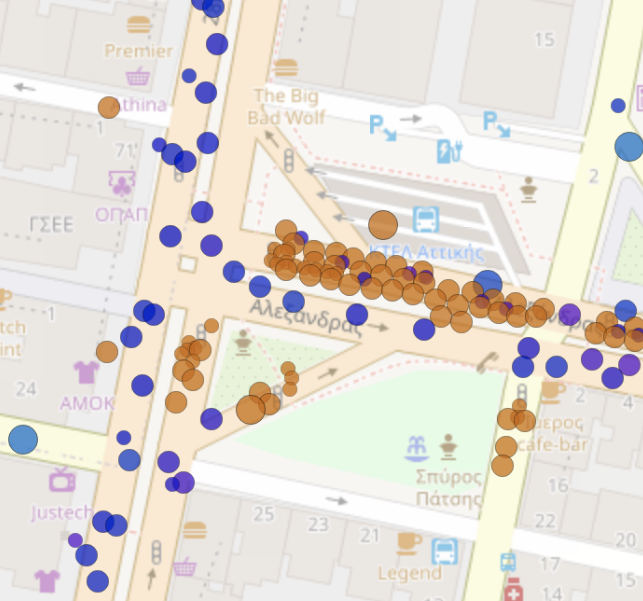
\includegraphics[width=.8\linewidth]{1s.png}  
  \caption{1s}
  \label{fig:sub-first}
\end{subfigure}
\begin{subfigure}{.5\textwidth}
  \centering
  % include second image
  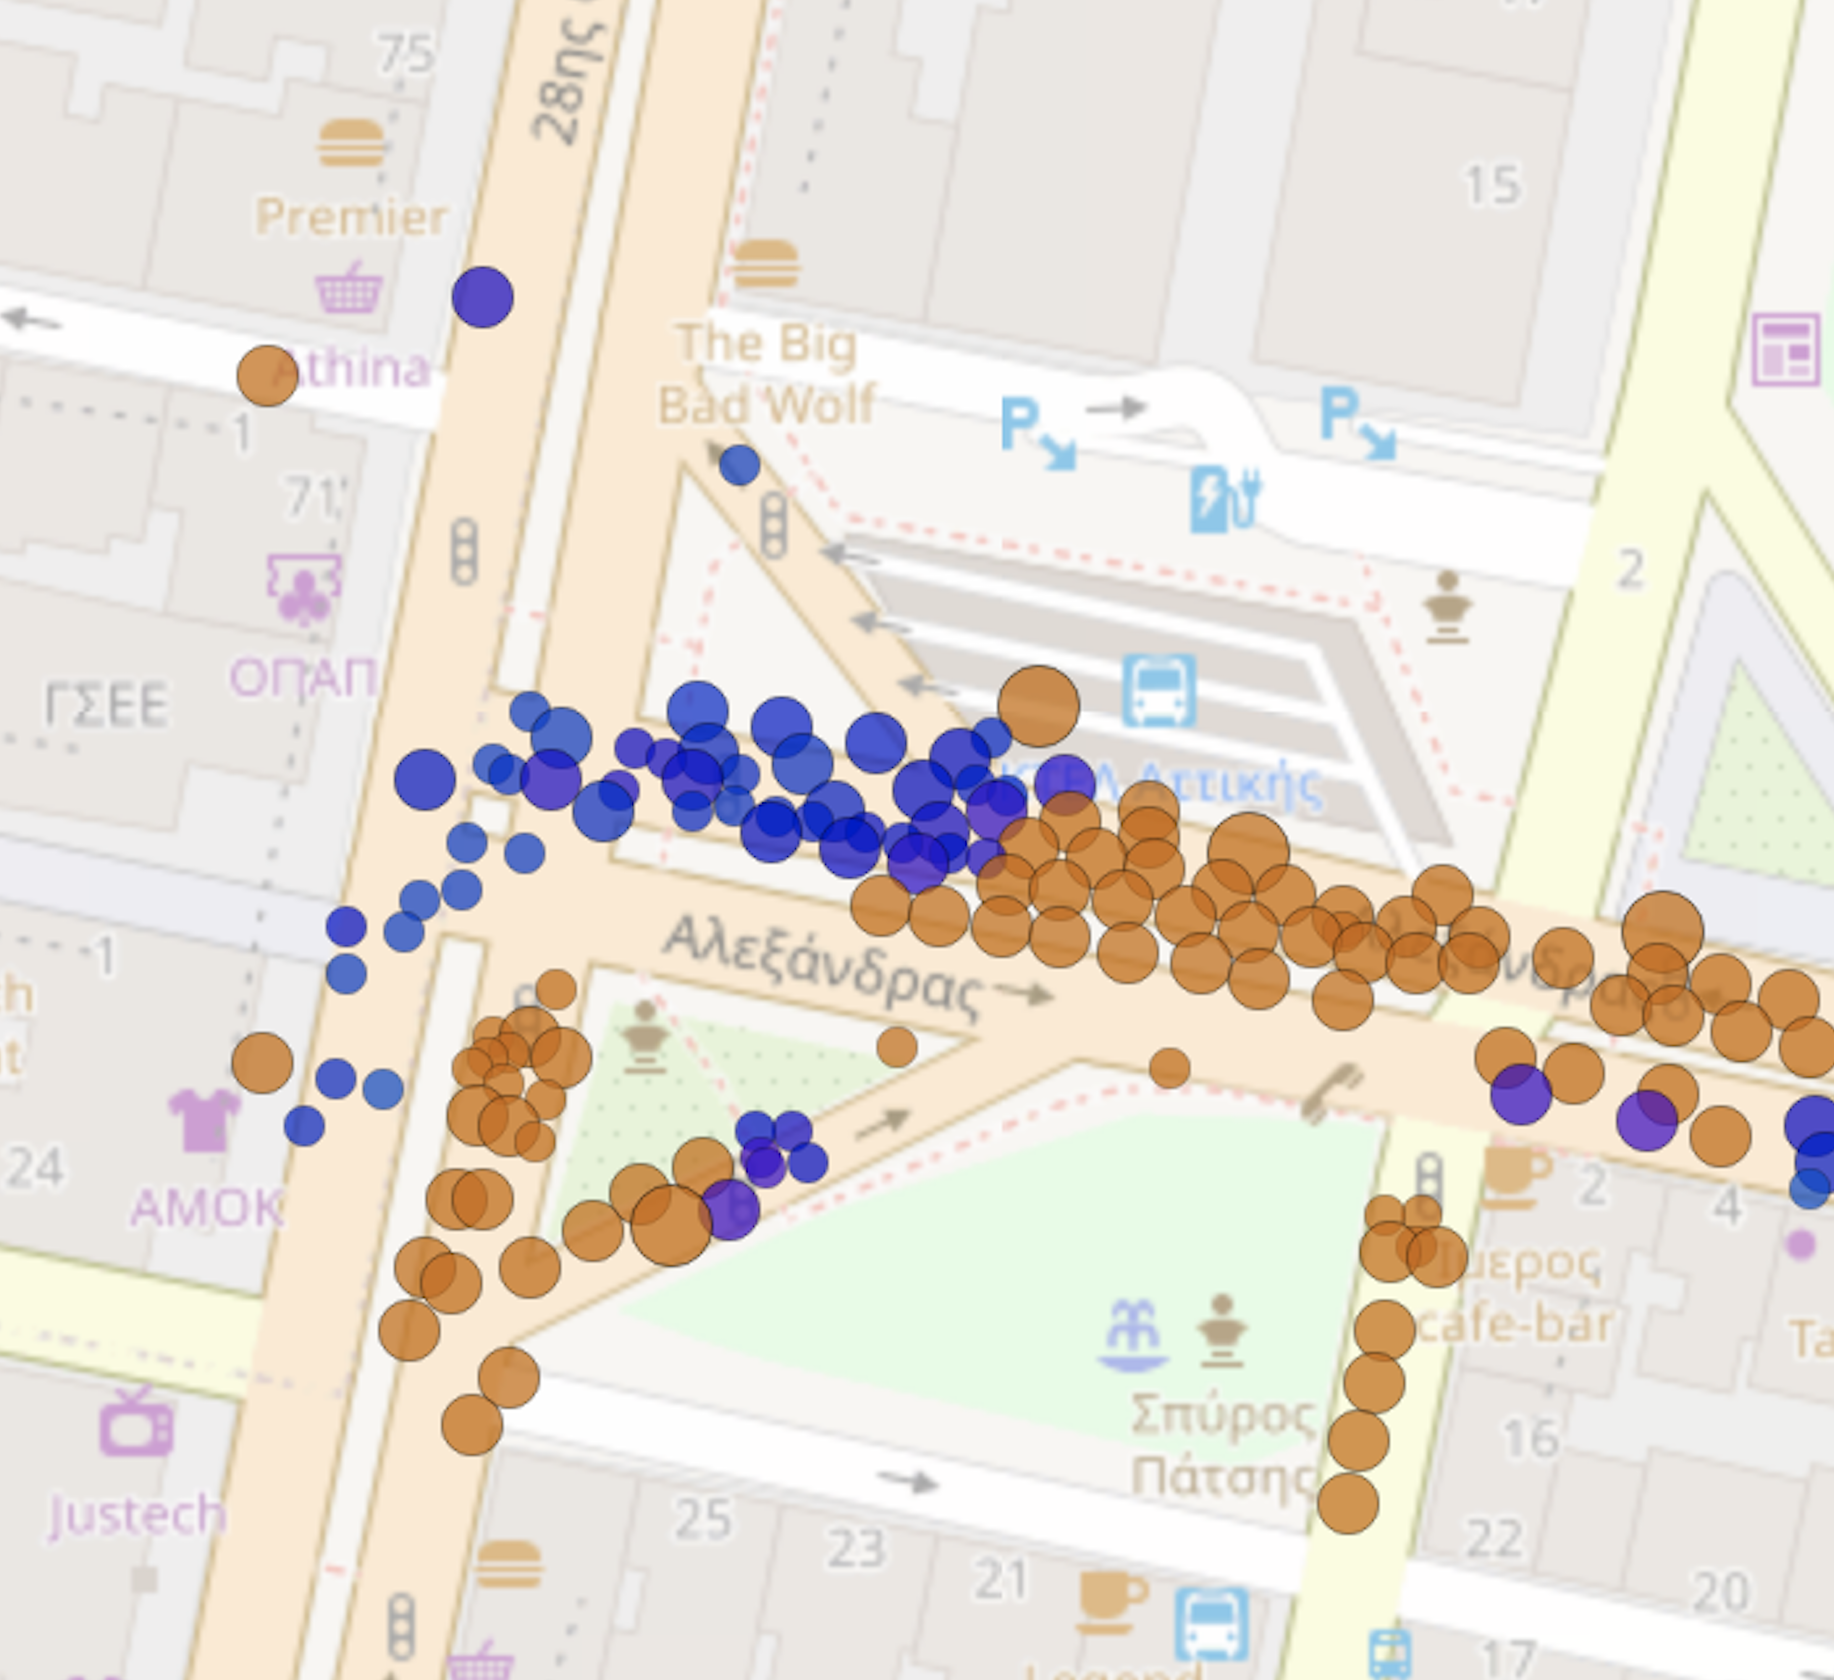
\includegraphics[width=.8\linewidth]{11s(1).png}  
  \caption{11s}
  \label{fig:sub-second}
\end{subfigure}

\newline

\begin{subfigure}{.5\textwidth}
  \centering
  % include third image
  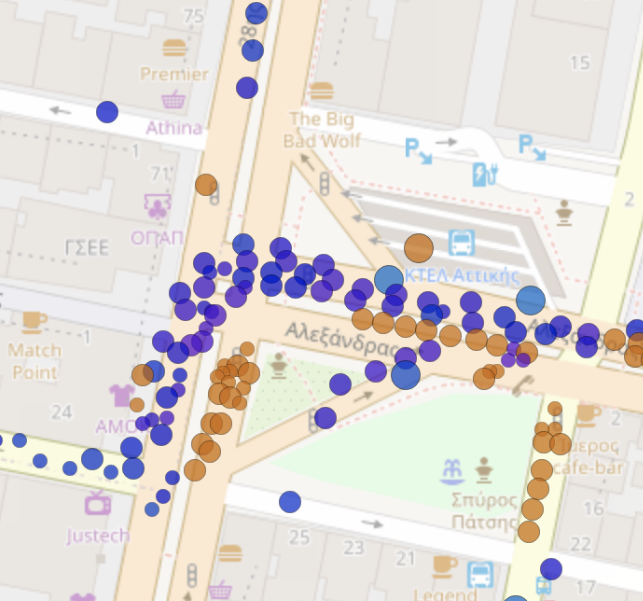
\includegraphics[width=.8\linewidth]{21s.png}  
  \caption{21s}
  \label{fig:sub-third}
\end{subfigure}
\begin{subfigure}{.5\textwidth}
  \centering
  % include fourth image
  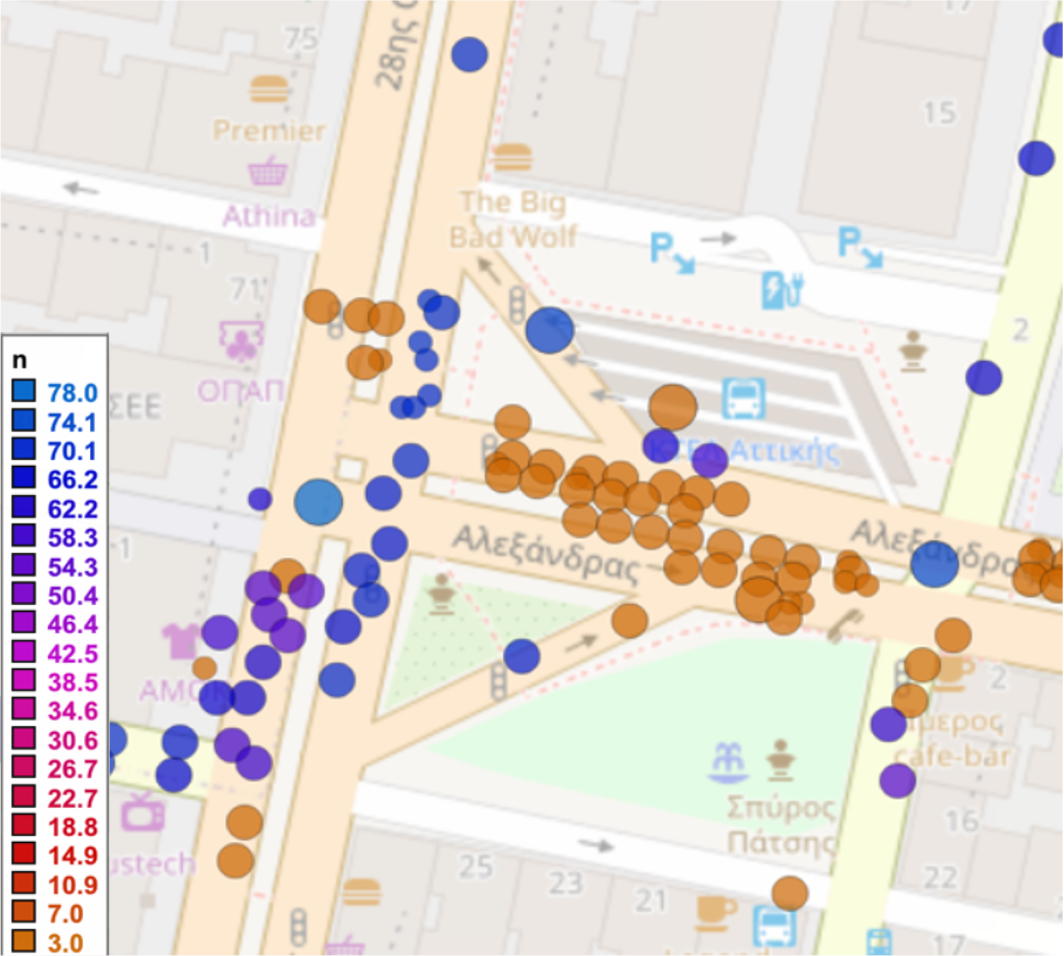
\includegraphics[width=.8\linewidth]{31s(1).png}  
  \caption{31s}
  \label{fig:sub-fourth}
\end{subfigure}
\caption{The noise emission distribution in Athens city map}
\label{fig:fig}
\end{figure}
\noindent In order to find out the noise emission influence of vehicles in real city map, the heat map is plotted based on the Athens city map in Figure \ref{fig:fig}. An intersection is analysed in one red light loop in the road of east direction. From the analysis above, these 3 models have similar assumptions for calculating the noise emission from each vehicle. However, since the static vehicle is considered as producing no noise emission based on the NMPB model, but the other 2 models regard these vehicles as producing the noise even they are not moving. Therefore, this section will take NMPB into account as its assumption is more practical compared to the other 2 models.

\noindent At the beginning of the intersection, there is queues waiting in the road of the east direction and south direction, the vehicle in the road of the north  direction could move freely. In the heat map, there are few noise emission in the east direction except one bus and several motorcycles, because bus can drive in the bus lane, and motorcycles do not need to wait in front of the red light. In the road of north direction, several vehicles create noise emission because they are moving, besides, the vehicle who is turning around could create fewer noise emission than the vehicle who is moving straight, because these vehicles who turns around have to decelerate.

\noindent After 10 seconds, the vehicles in the east direction could move, it could be seen that the vehicle who moves first create higher noise emission than the vehicle who starts to accelerate from static state, because the vehicle who moves first has higher speed and also it is accelerating. Since the vehicles far from the intersection are not moving, they do not create any noise.

\noindent After 20 seconds, since all the vehicles in the east direction road are moving to turn left, all the vehicles in the road produce noise emission, and among these vehicles, heavy vehicles create more noise emission than the light vehicles. 

\noindent After 30 seconds, the vehicles passing the intersection continue to produce noise emission, however, the vehicles who have not passed the intersection stop producing the noise emission because the light is turning red again.
{\color{red} \subsection{Results of data aggregation of road segments}}
\subsubsection{Analysis between the equivalent line sound power level, speed and flow }
\noindent Since the equivalent line sound power level has been introduced in the previous section. In this part, the relationship between the line sound power of one vehicle and its speed and flow will be analyzed, the data of 120 seconds from 2 different vehicles are chosen, the results are shown in Figure \ref{line sound power}:
\begin{figure}[h]
     \centering
     \begin{subfigure}[h]{0.47\textwidth}
         \centering
         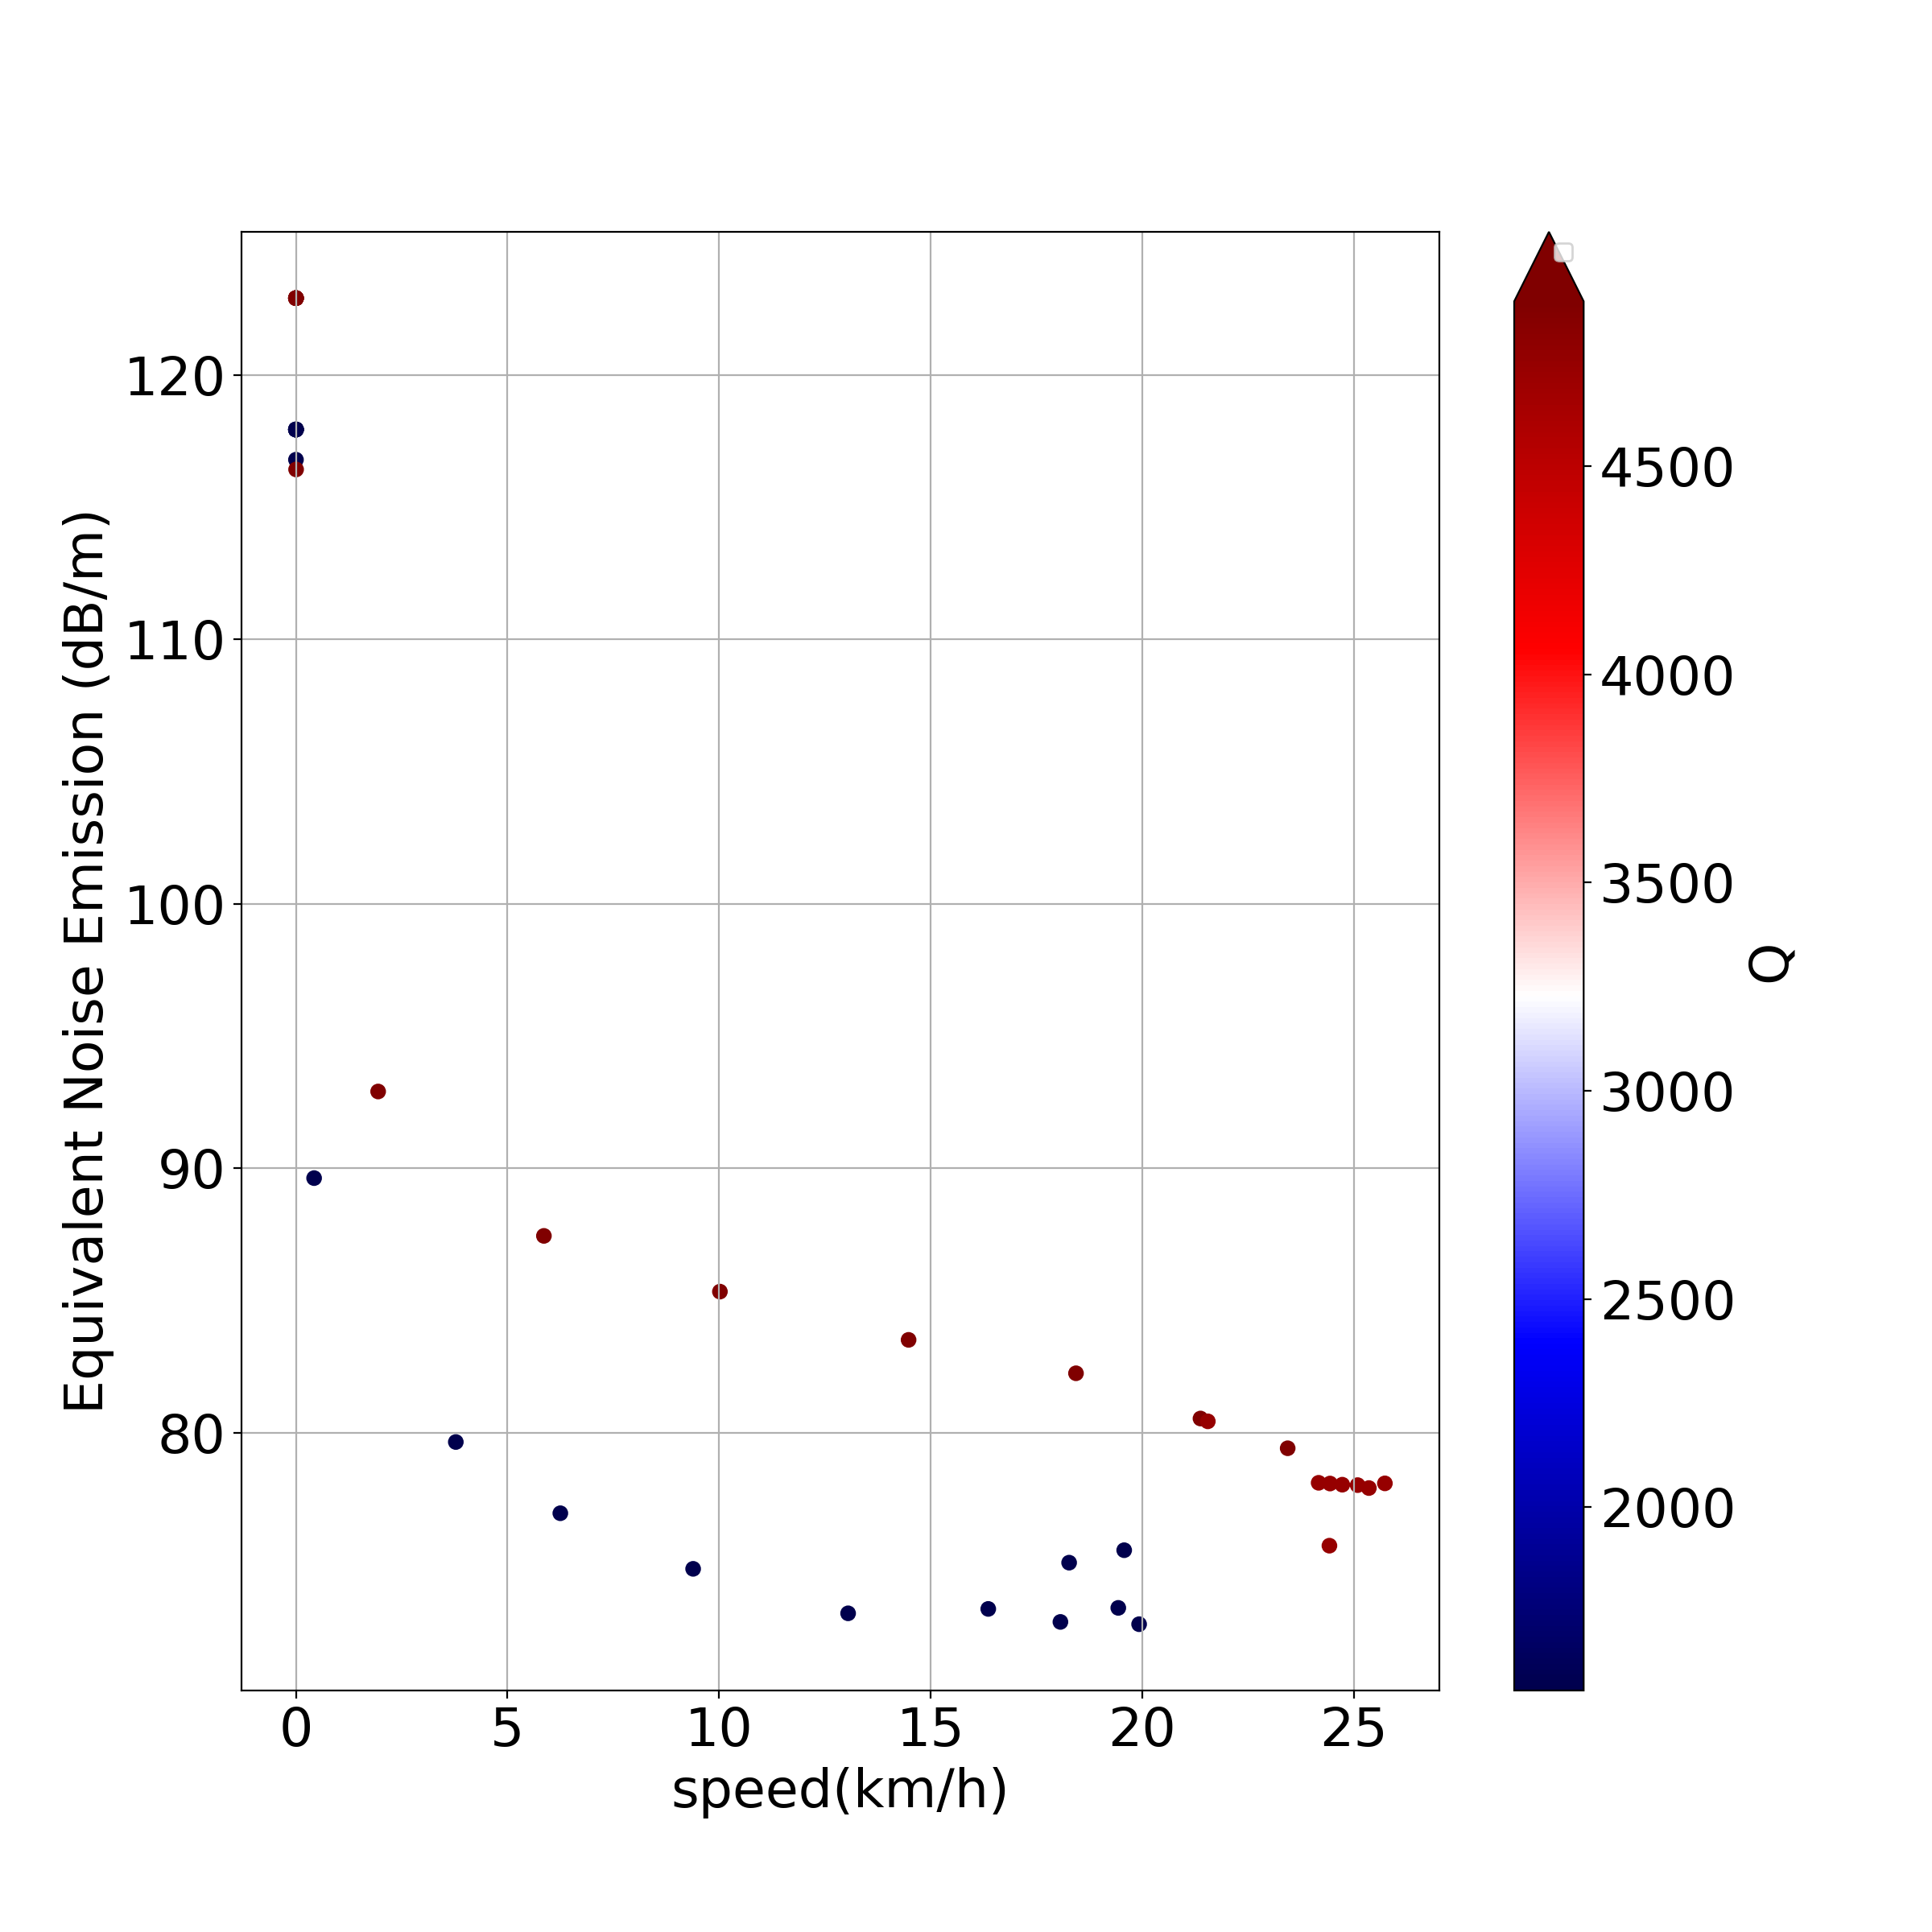
\includegraphics[width=\textwidth]{emission-speed-flow(bus).png}
         \caption{Bus}
         \label{R2L}
     \end{subfigure}
     \hfill
     \begin{subfigure}[h]{0.47\textwidth}
         \centering
         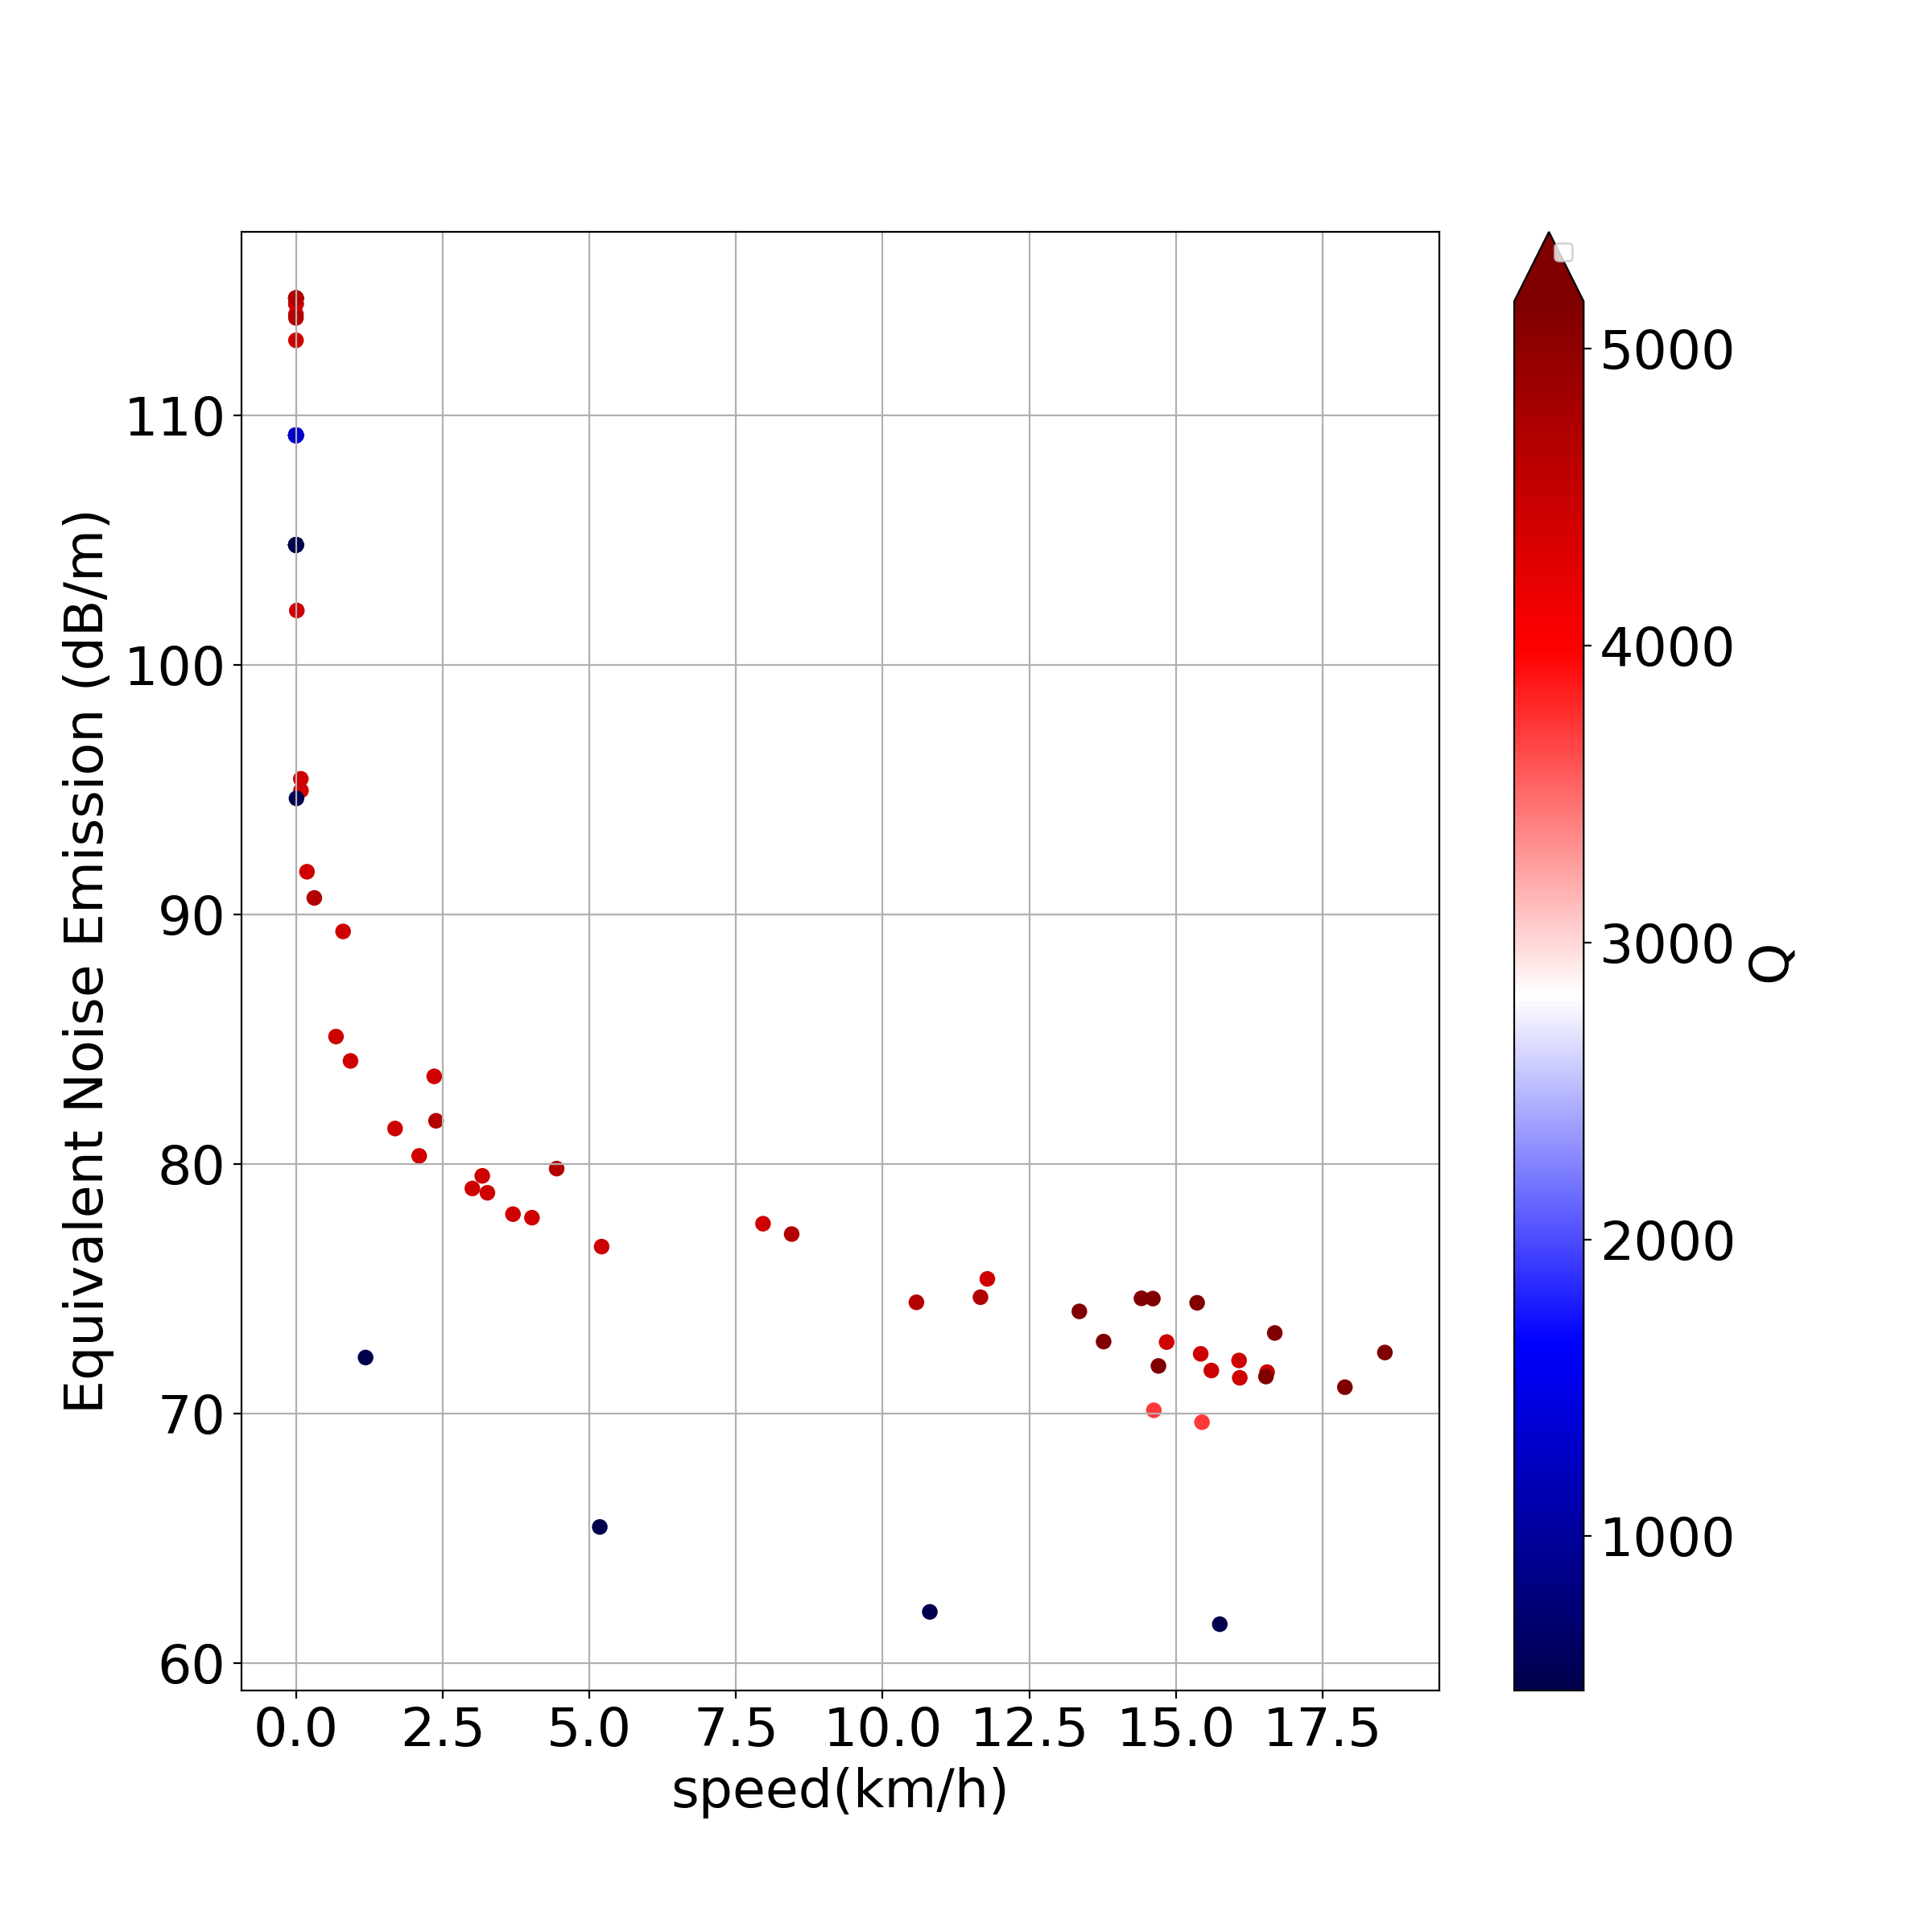
\includegraphics[width=\textwidth]{emission-speed-flow(Taxi).png}
         \caption{Taxi}
         \label{L2R}
     \end{subfigure}
\caption{The analysis of the equivalent line sound power}
\label{line sound power}
\end{figure}

\noindent From the graph, it could be observed that with the increasing of the speed, the $L_{W,line,eq}$ is decreasing, because the definition of $L_{W,line,eq}$ includes the influence of the pass-by time of the vehicle. Therefore, a vehicle passing by at a lower speed will be heard longer, which has an increasing effect on the equivalent sound power level $L_{W,line,eq}$. Besides, 2 curves were observed in the graph, with the increasing of the flow $Q$, the $L_{W,line,eq}$ is also increasing.
\noindent Based on the calculation of $L_{W,line,eq}$ above, the road segment noise level could be calculated based on the data aggregation method.
\newpage
\subsubsection{Analysis of noise emission in road segment }

\noindent In the previous section, the data aggregation method is introduced for calculating the equivalent noise emission for road segment. In this section, all the segment in a specific road is analysed by the IMAGINE model and the CNOSSOS model.

\begin{figure}[h]
     \centering
     \begin{subfigure}[H]{0.47\textwidth}
         \centering
         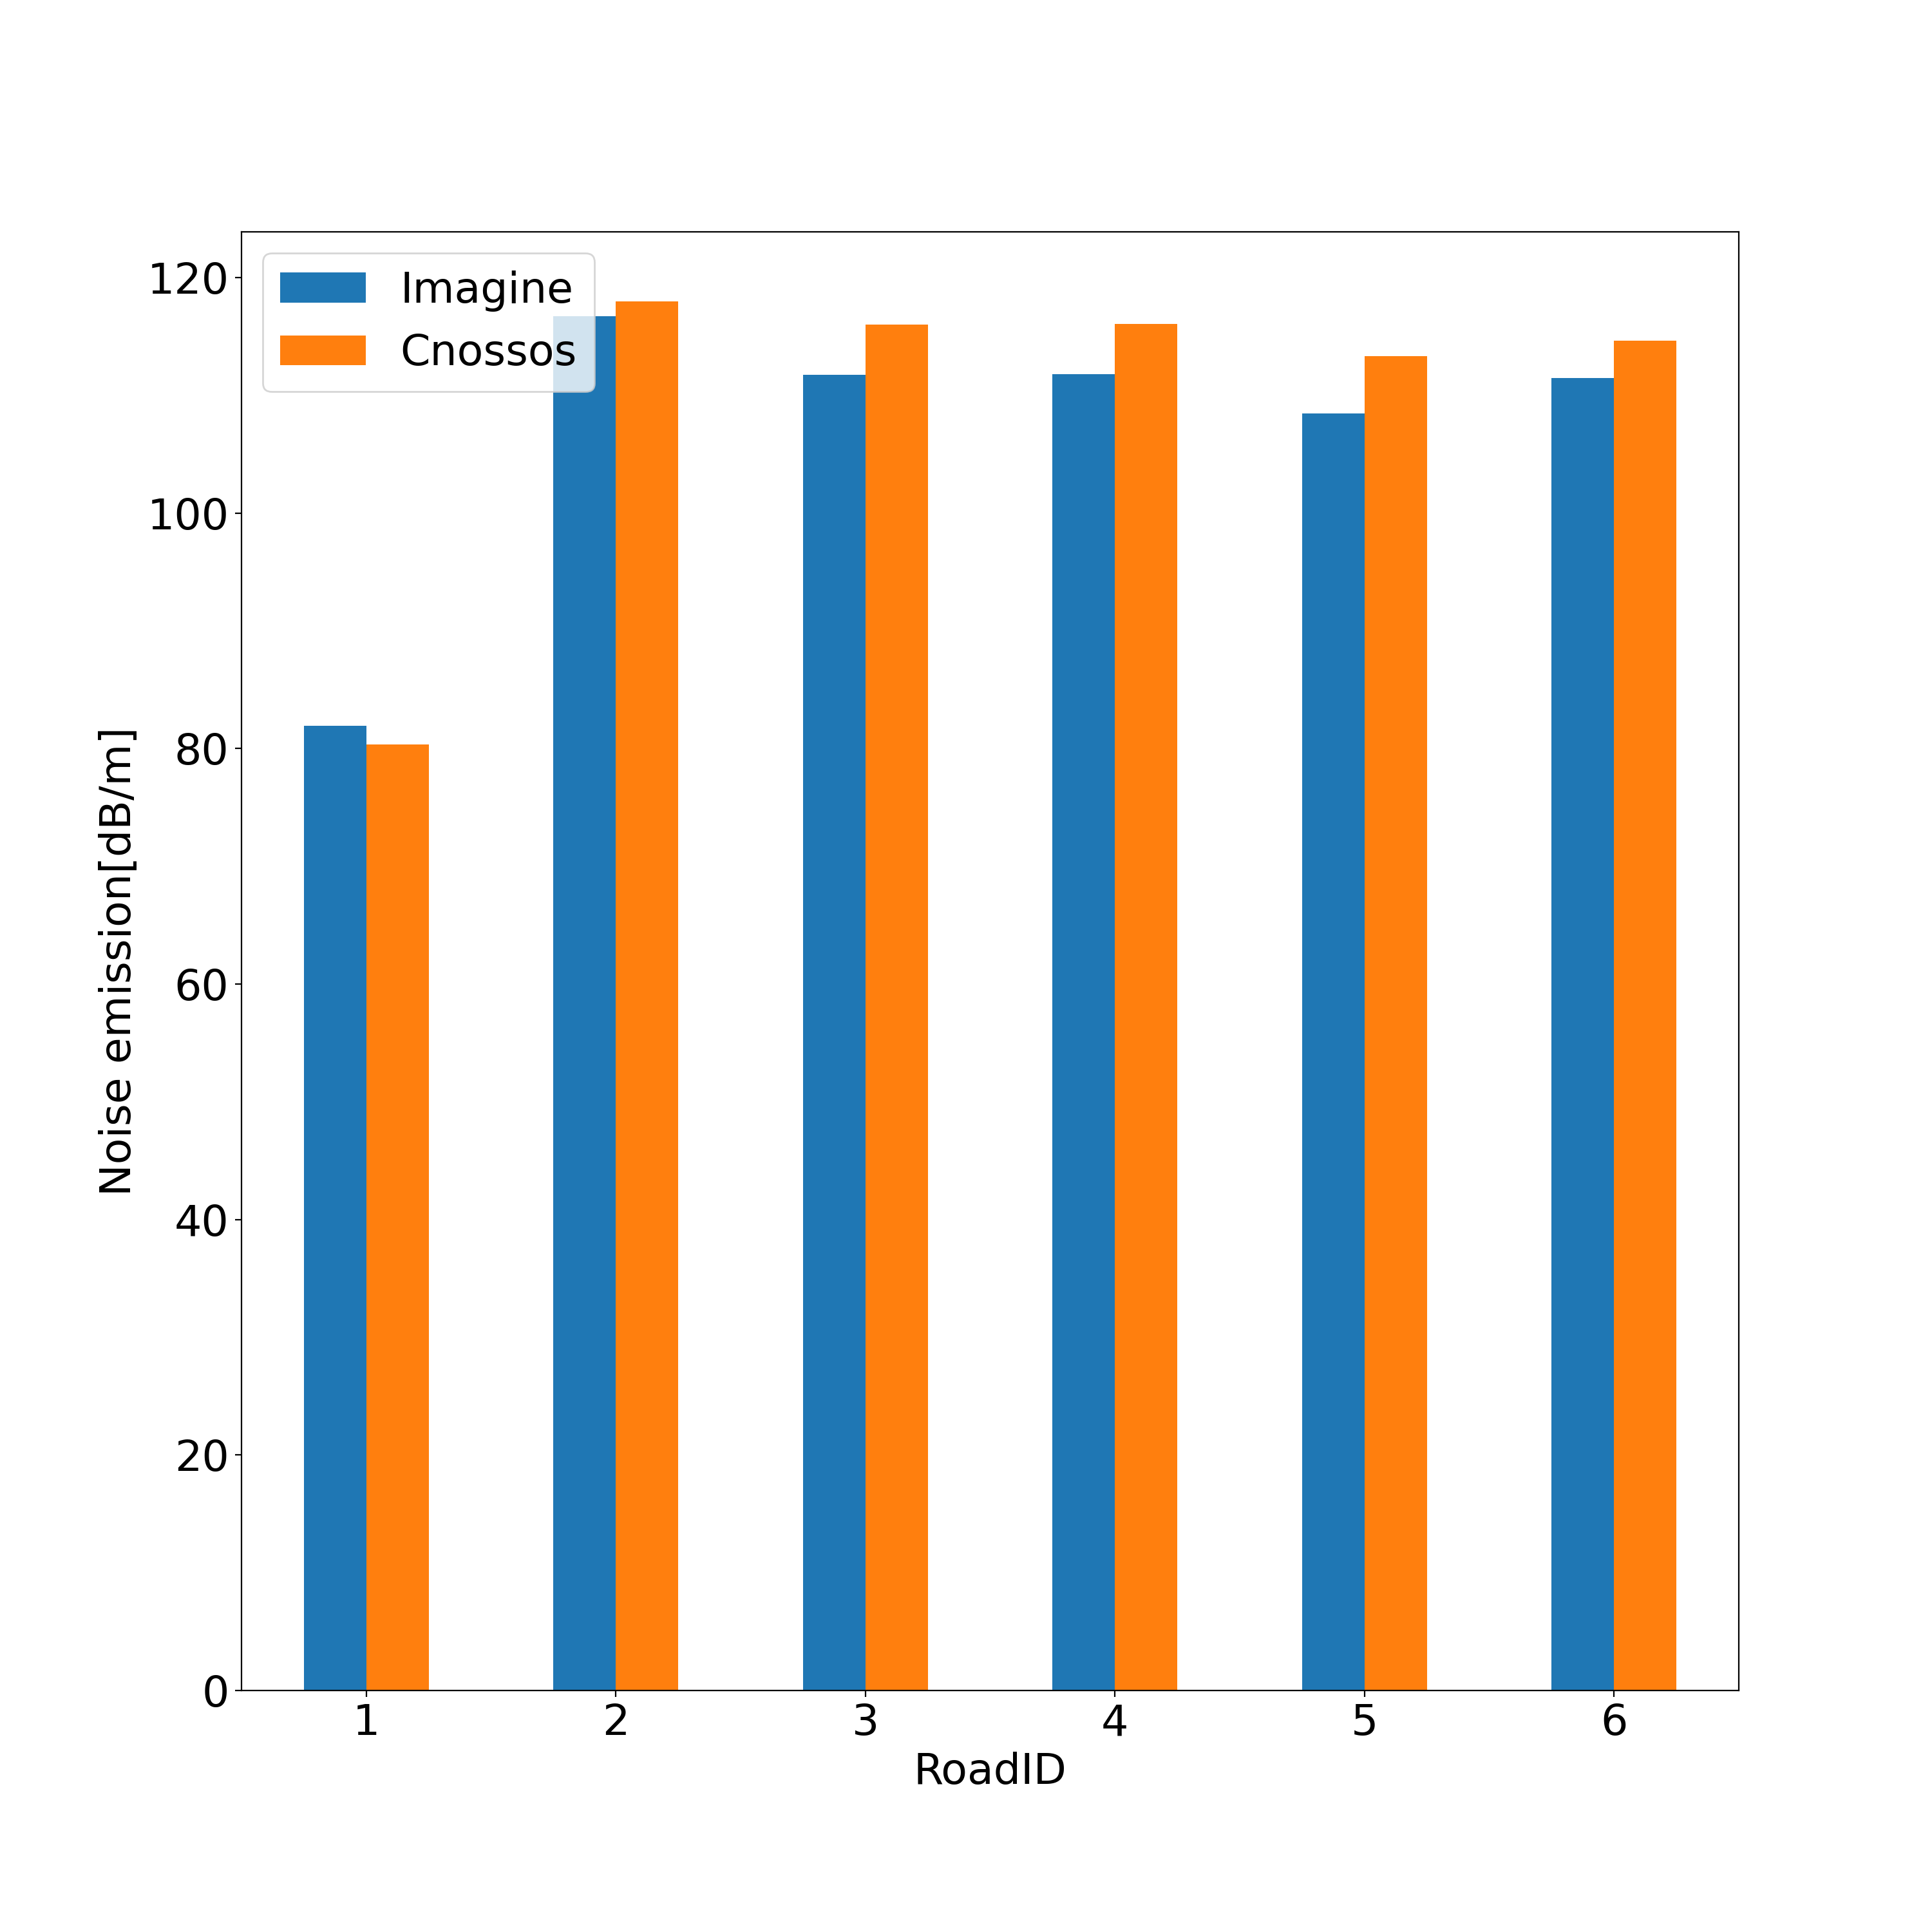
\includegraphics[width=\textwidth]{first30s(up).png}
         \caption{direction: east to west}
         \label{R2L}
     \end{subfigure}
     \hfill
     \begin{subfigure}[H]{0.47\textwidth}
         \centering
         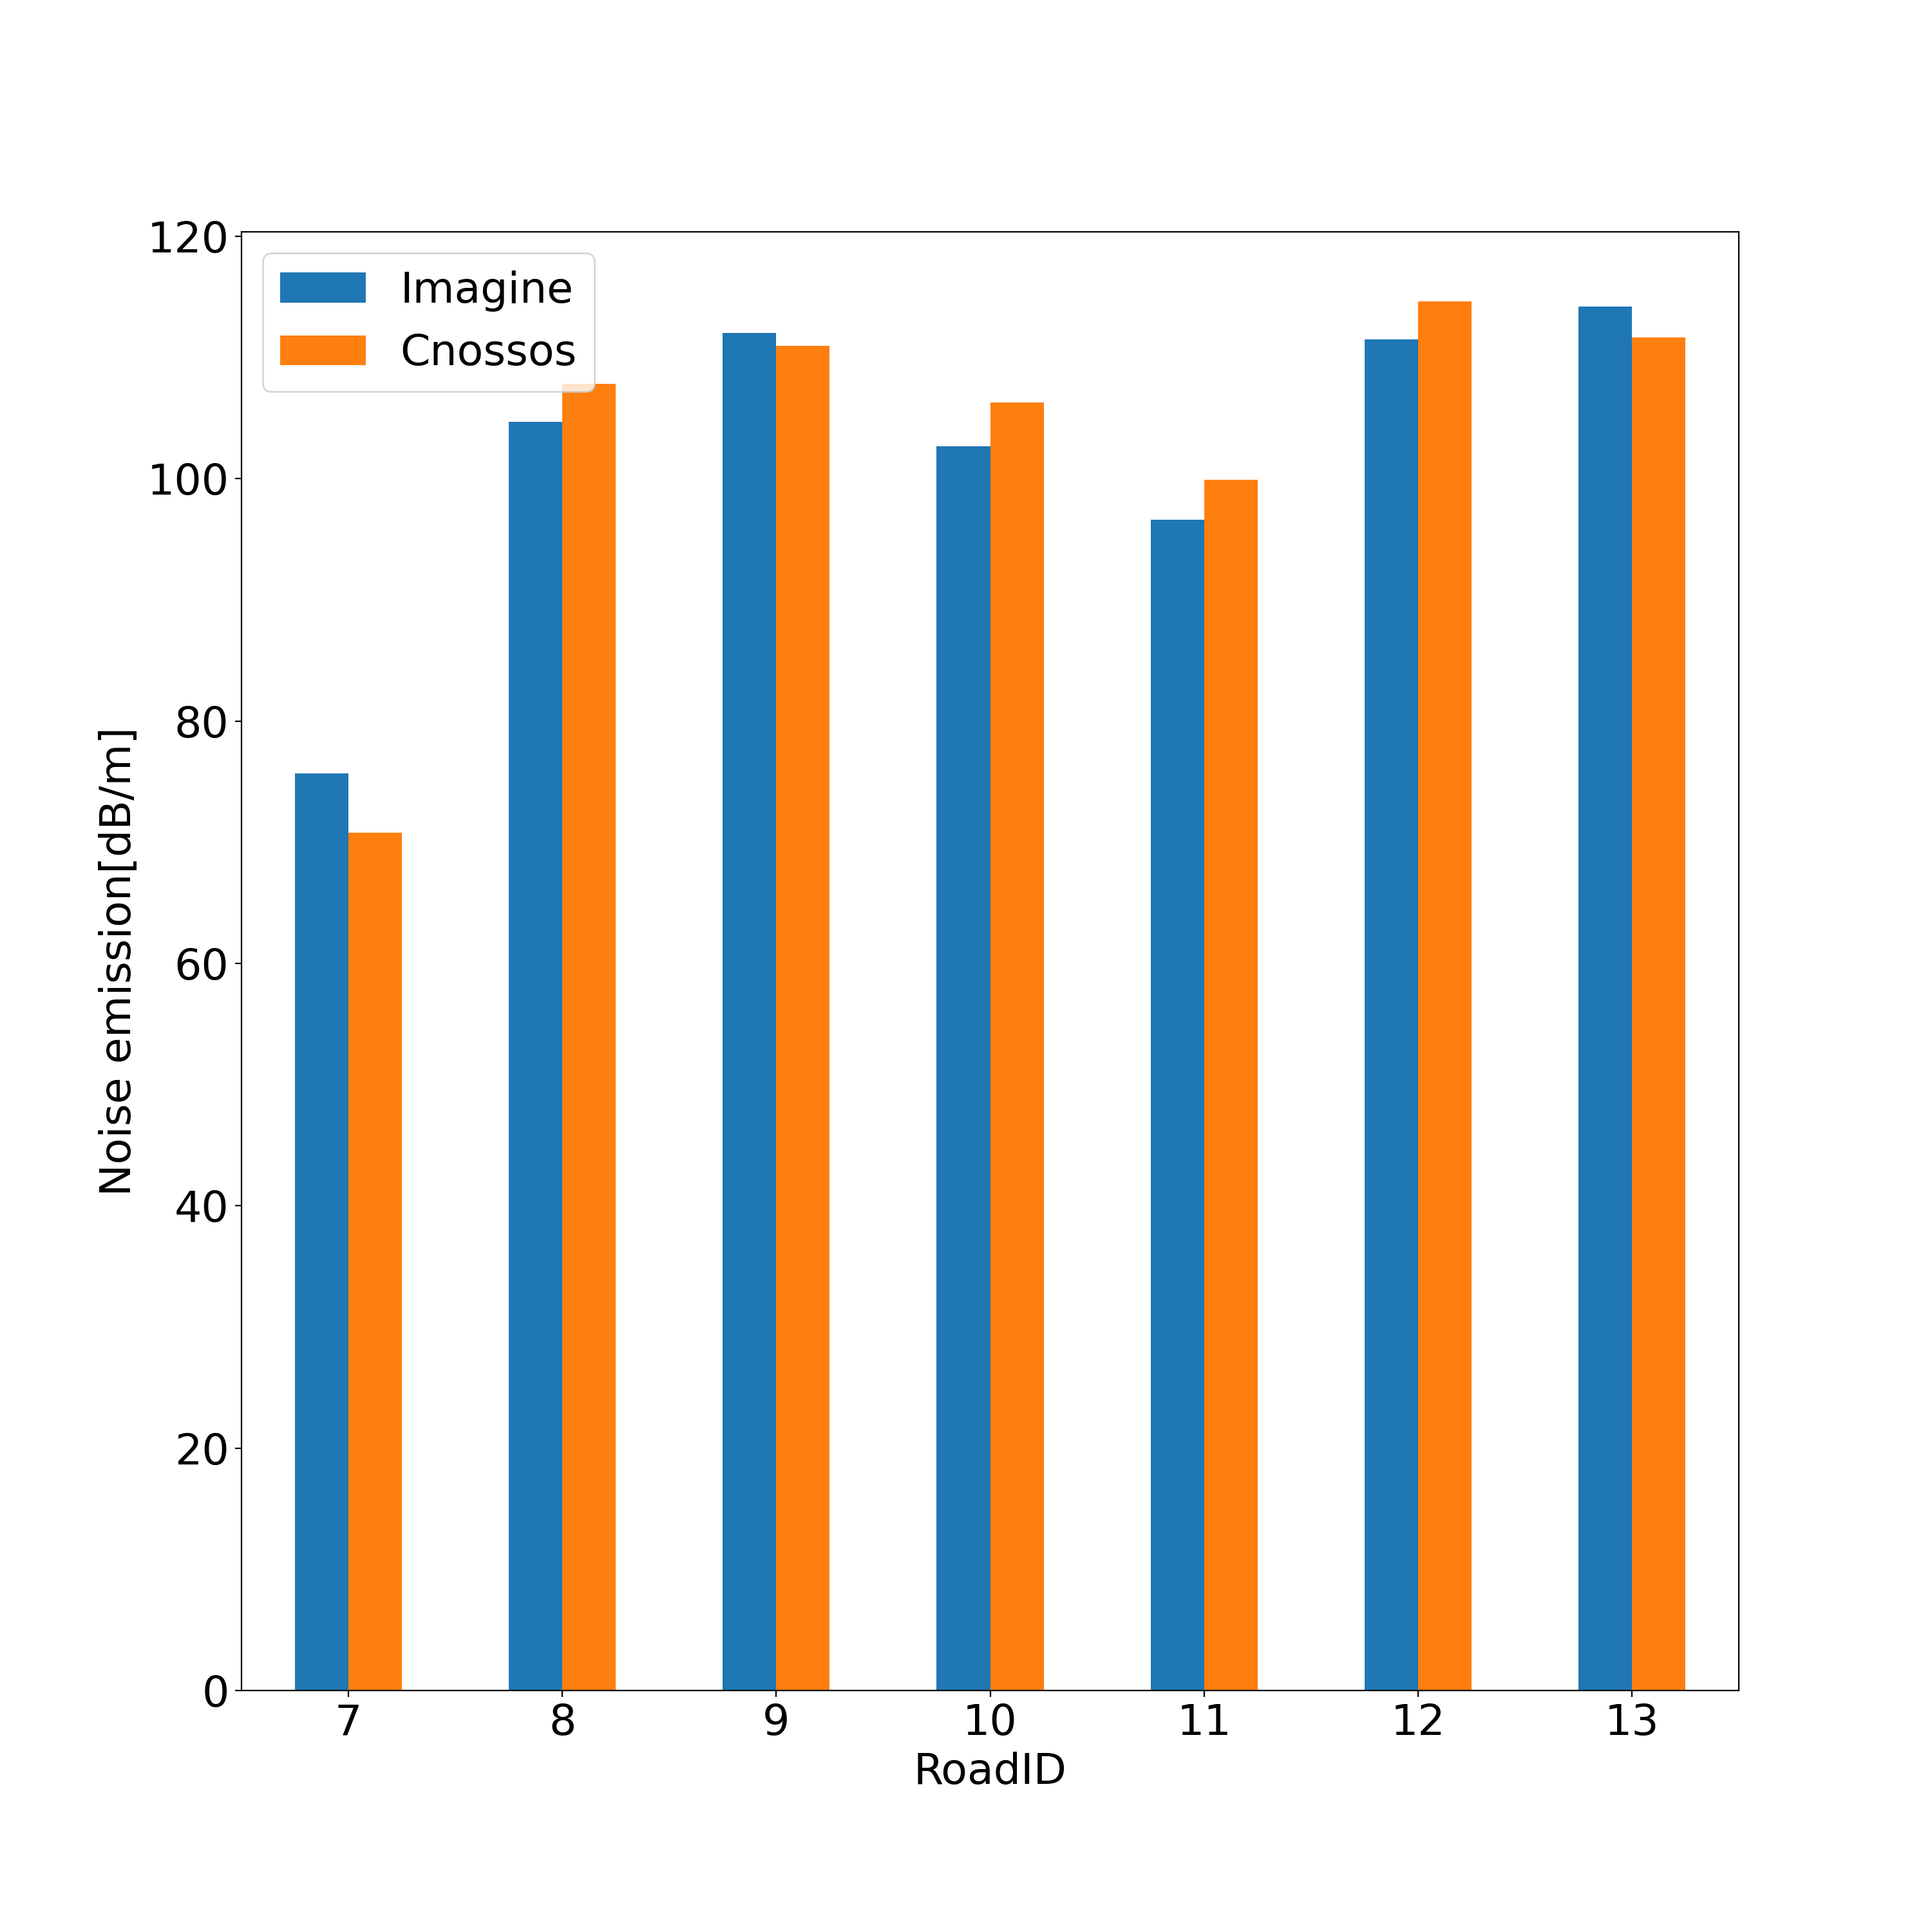
\includegraphics[width=\textwidth]{first30s(down).png}
         \caption{direction: west to east}
         \label{L2R}
     \end{subfigure}
\caption{{\color{red} Segments}}
\label{Segments in target road}
\end{figure}
\begin{figure}[h]
    \begin{center}
        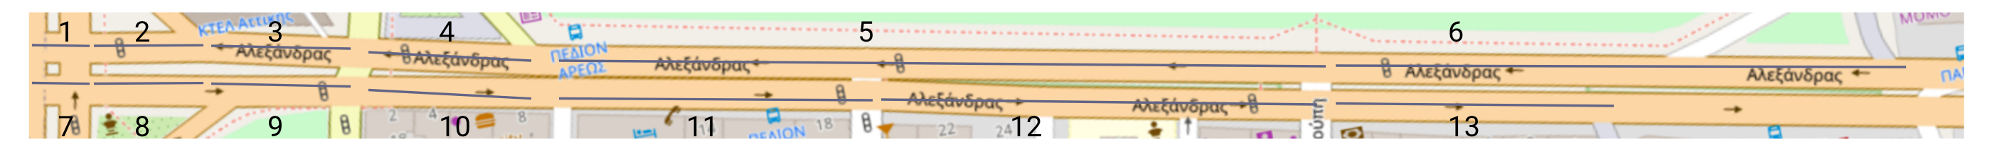
\includegraphics[width=\textwidth]{road11.png}
        \caption{The location of selected roads}
        \label{road11}
    \end{center}
\end{figure}

\noindent The Figure \ref{Segments in target road} represents the average noise emission effect in each open street map segment based on the calculation of one cycle(90 seconds), the left graph represents the road whose direction is from east to west, the right graph represents the road whose direction is from west to east. It can be seen that the CNOSSOS model will calculate a higher value for road segment noise emission in most situations, which is corresponding to the previous analysis for individual vehicle noise emission. Besides, the noise emission of the 2 segments in the west is smaller than the other segment, because the vehicles driven in these segments have to be in a relatively high speed, they will be heard shorter in these segments. The noise emission produced in these segments is relatively small.
\begin{figure}[h]
     \centering
     \begin{subfigure}[H]{0.45\textwidth}
         \centering
         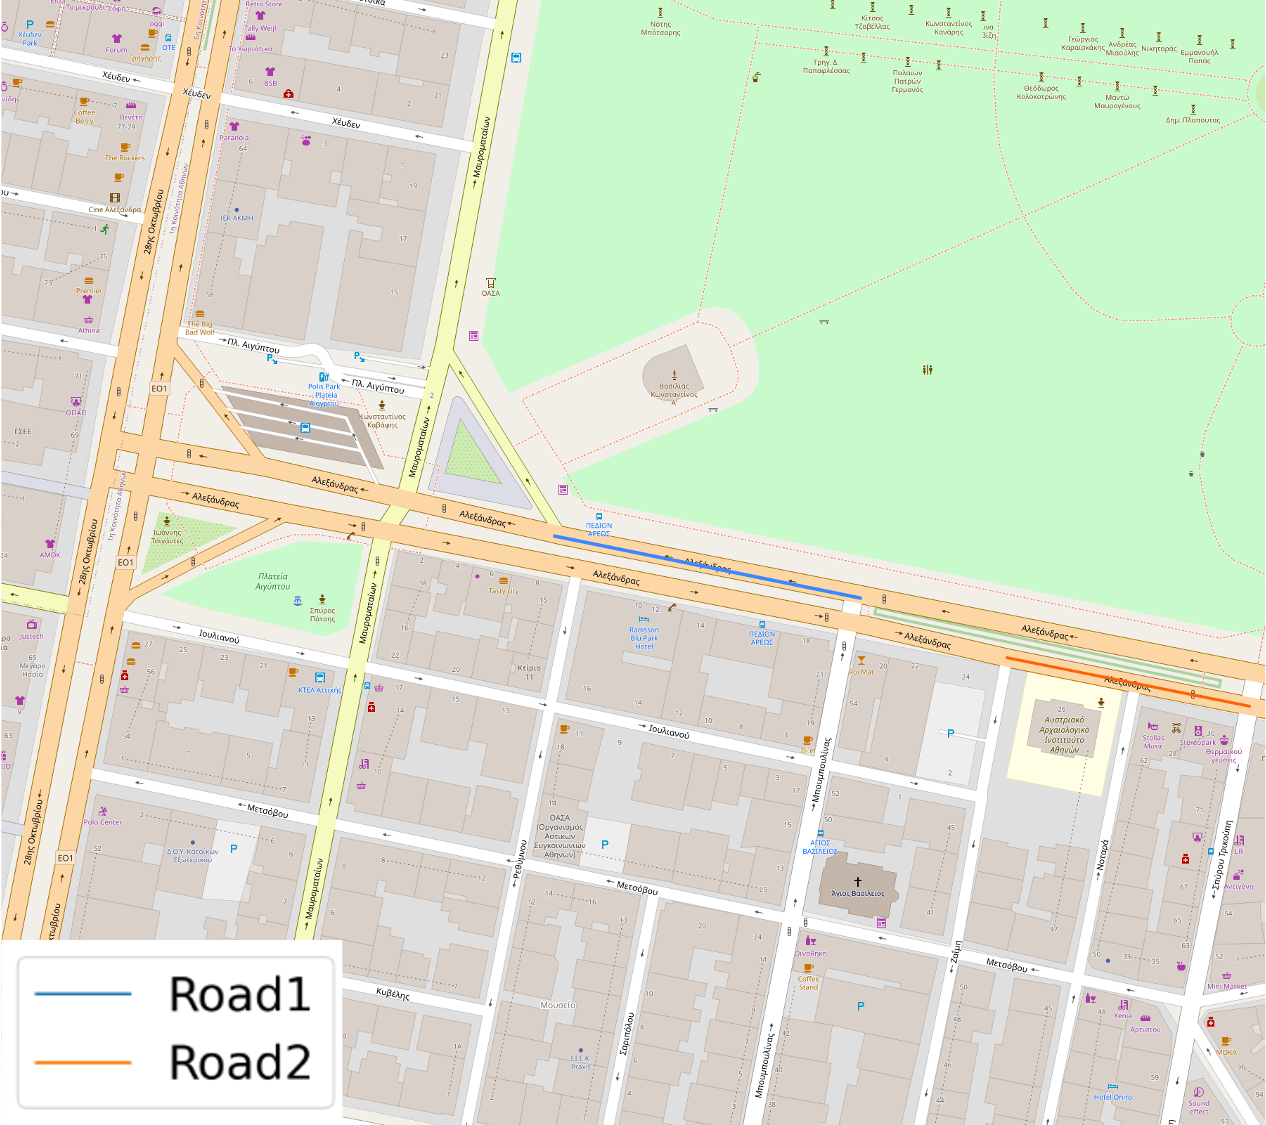
\includegraphics[width=\textwidth]{road.png}
         
         \label{r1}
     \end{subfigure}
     \hfill
     \begin{subfigure}[H]{0.52\textwidth}
         \centering
         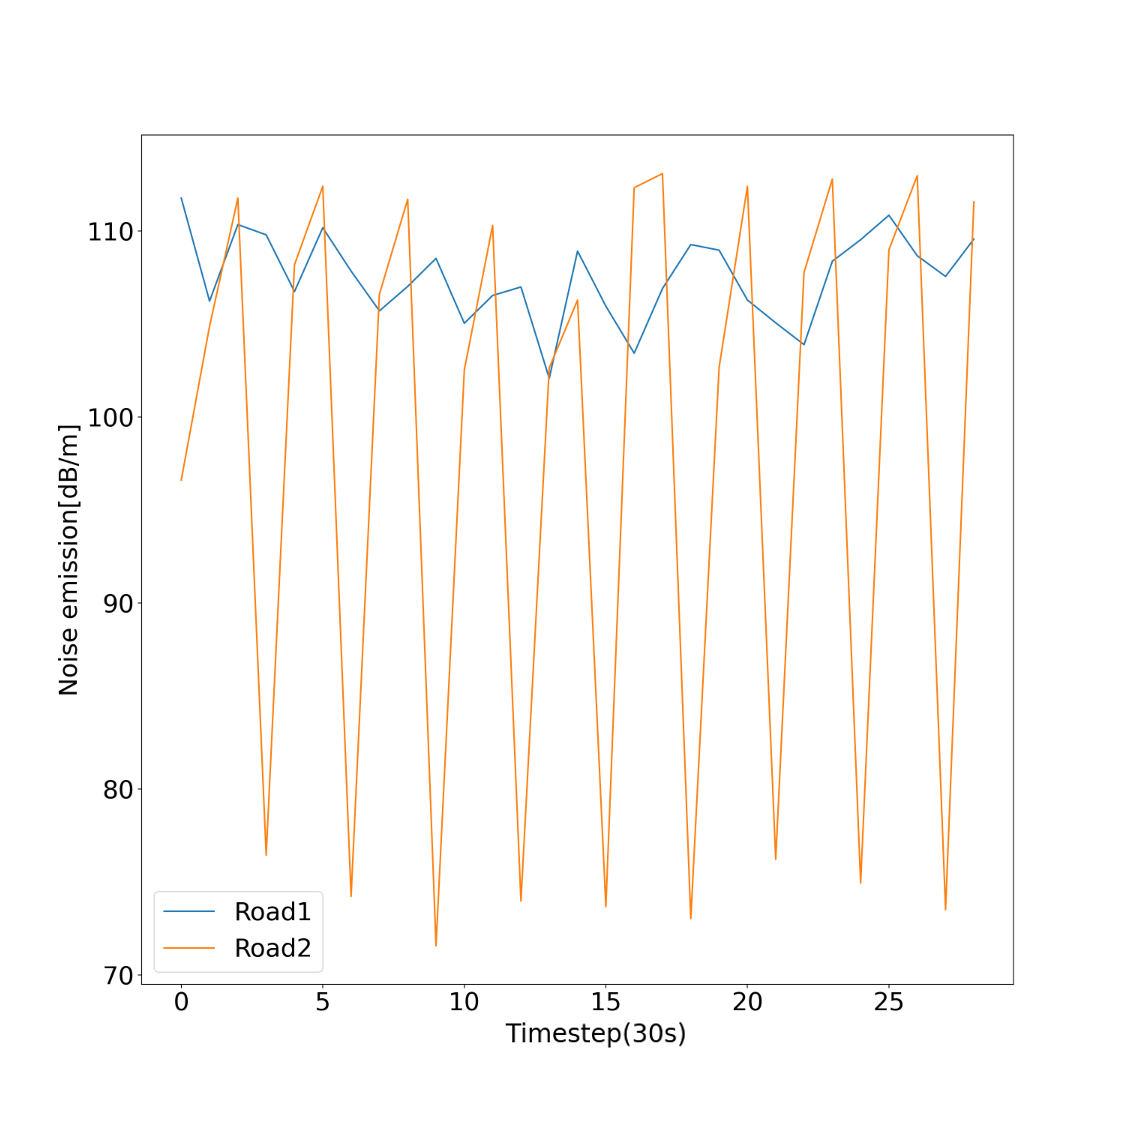
\includegraphics[width=\textwidth]{t vs noise.png}
         
         \label{r2}
     \end{subfigure}
\caption{Left:The location of 2 segments. Right:Periodicity effect of the road segment}
\label{Periodicity}
\end{figure}

\noindent In order to analyse the periodicity of the noise emission of the road segment, the time step is reset as 30 seconds, and the equivalent noise emission of each road segment is calculated again. Two segments are chosen, which are shown in the left of the Figure \ref{Periodicity}. The pattern of these two roads can be observed in the right of the Figure \ref{Periodicity} that each segment produces different noise emission in one cycle(90 seconds), but the noise emission distribution of different cycle are similar. The reason for the pattern difference of these two roads are explained below:
{\color{red}
\begin{itemize}
    \item For the road 1, in the first 30 seconds, the traffic light in front of this road just turn red, which means the queue is starting to grow. Therefore, the vehicles in the behind of the road can still move and produce the noise. In the second 30 seconds, the road 1 is fully occupied by vehicles, as they are still waiting for the queue, the noise emission of road 1 is lower than first 30 seconds. In the last 30 seconds, the traffic light turns green, all the vehicles staying in this road can move again and produce noise. Therefore, the noise emission for the last 30 seconds is higher than the second 30 seconds.
    \item For the road 2, in the first 30 seconds, there are not so many vehicles in this road, as the queue is almost dissipating. Therefore, the vehicles can move in a free road speed, which could create fewer noise emission. In the second 30 seconds, the traffic light turns red, the new vehicles arriving in this road have to decrease their speed and stop. It could produce lower noise emission for one vehicle,  however, based on the analysis of section 9.5.1, the noise emission produced by segment is higher if the average speed for the vehicles in this road is low. Therefore, it is reasonable that the road 2 produces higher noise emission in the second 30 seconds than the first 30 seconds. In the last 30 seconds, the traffic light behind the road 2 turns green, the queue behind road 2 is released, so the flow of the road 2 is increasing, then the traffic light in front of the road 2 also turns green, all the vehicles in the road 2 can move. Because of the high flow of this road and the vehicles start to move, the noise emission of the last 30 seconds is higher than the second 30 seconds.
\end{itemize}
}


\section{Conclusion}
{\color{red}

This project relies on the real vehicles trajectories collected by multiple drones (speed and acceleration of vehicles with a 1 s granularity), to estimate sound power level as well as sound pressure levels along the road. Based on the traffic data and different noise emissions models, the sound power levels and the sound pressure level could be analyzed in different ways, and several results are obtained:
\begin{itemize}
    \item Significant differences are observed according to the choice of the model, with regard to the vehicle acceleration, the IMAGINE model and CNOSSOS model show greater flexibility in the calculation, because they regard the accelerating state as a continuous value rather than a discrete value (accelerating, decelerating or steady condition).
    \item The heat map of the noise distribution is plotted and analyzed, the noise emission of single vehicle is estimated according to the location and time, the pattern for vehicles is observed within an intersection.
    \item Sound pressure level is estimated and compared in several roads within one traffic light cycle, the periodicity pattern for each road is noticed because of the periodicity pattern of the traffic light.
\end{itemize}
}
\section{Appendix}
\begin{figure}[H]
    \begin{center}
        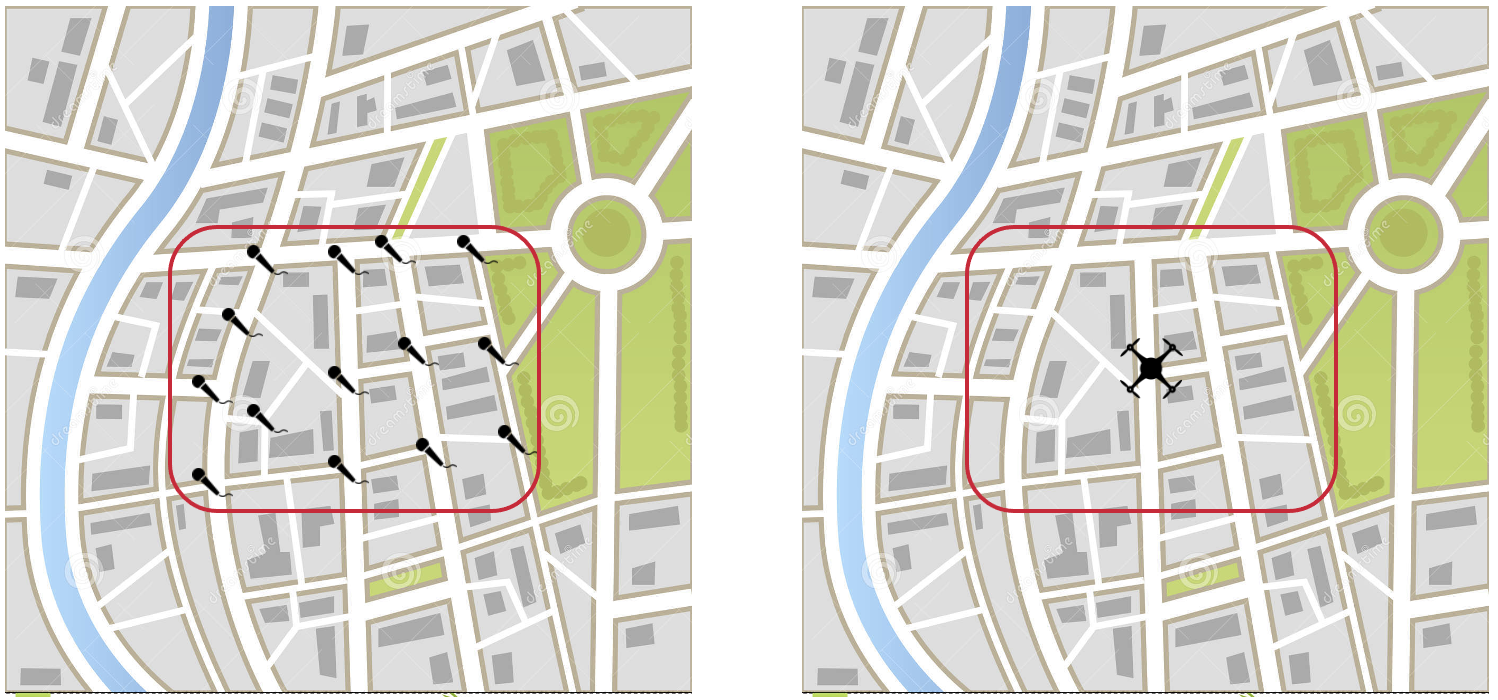
\includegraphics[width=14cm]{City noise emissions monitoring.png}
        \caption{City noise emissions monitoring}
        \label{City noise emissions monitoring}
    \end{center}
\end{figure}

\begin{figure}[H]
    \begin{center}
        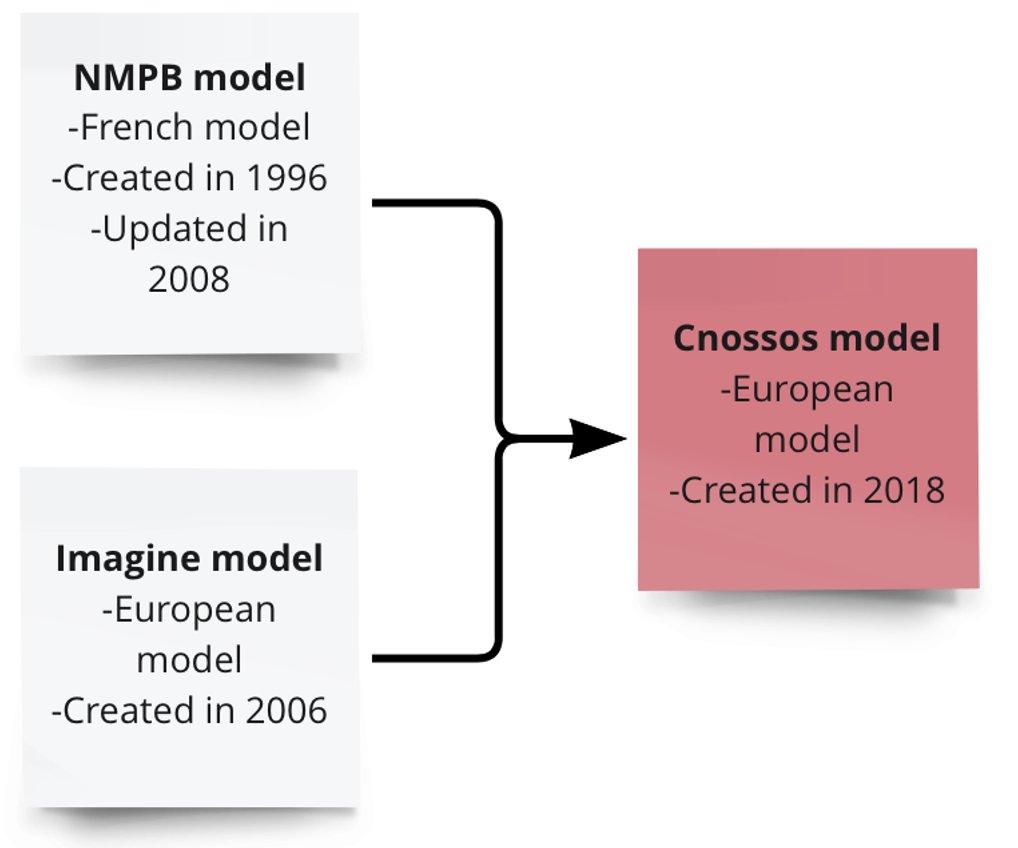
\includegraphics[width=14cm]{Noise emissions models.png}
        \caption{Noise emissions models}
        \label{Noise emissions models}
    \end{center}
\end{figure}

\begin{figure}[H]
    \begin{center}
        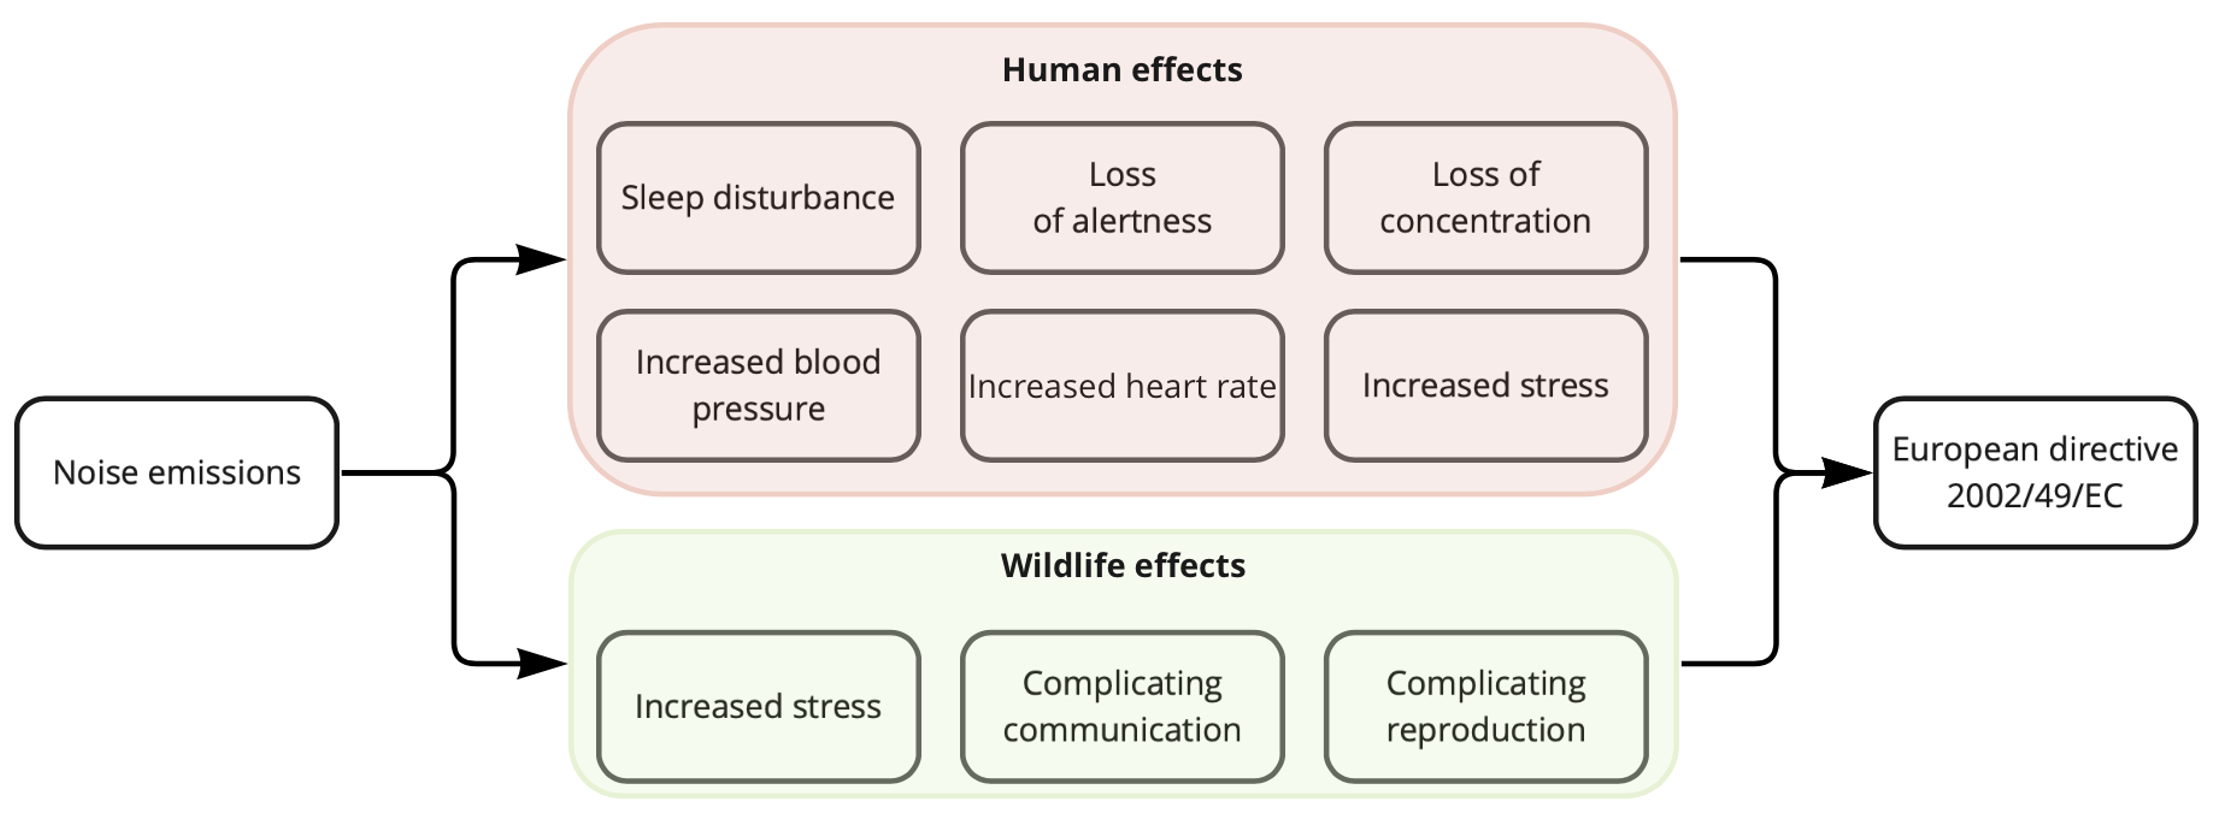
\includegraphics[width=14cm]{European noise emissions directive.png}
        \caption{European noise emissions directive}
        \label{European noise emissions directive}
    \end{center}
\end{figure}






\newpage
\bibliographystyle{IEEEtran}
\bibliography{ref}




\end{document}